%%%%%%%%%%%%%%%%%%%%%%%%%%%%%%%%%%%%%%%%%
% Masters/Doctoral Thesis 
% LaTeX Template
% Version 2.5 (27/8/17)
%
% This template was downloaded from:
% http://www.LaTeXTemplates.com
%
% Version 2.x major modifications by:
% Vel (vel@latextemplates.com)
%
% This template is based on a template by:
% Steve Gunn (http://users.ecs.soton.ac.uk/srg/softwaretools/document/templates/)
% Sunil Patel (http://www.sunilpatel.co.uk/thesis-template/)
%
% Template license:
% CC BY-NC-SA 3.0 (http://creativecommons.org/licenses/by-nc-sa/3.0/)
%
%%%%%%%%%%%%%%%%%%%%%%%%%%%%%%%%%%%%%%%%%

%----------------------------------------------------------------------------------------
%	PACKAGES AND OTHER DOCUMENT CONFIGURATIONS
%----------------------------------------------------------------------------------------

\documentclass[
11pt, % The default document font size, options: 10pt, 11pt, 12pt
oneside, % Two side (alternating margins) for binding by default, uncomment to switch to one side
english, % ngerman for German
singlespacing, % Single line spacing, alternatives: onehalfspacing or doublespacing
%draft, % Uncomment to enable draft mode (no pictures, no links, overfull hboxes indicated)
%nolistspacing, % If the document is onehalfspacing or doublespacing, uncomment this to set spacing in lists to single
%liststotoc, % Uncomment to add the list of figures/tables/etc to the table of contents
%toctotoc, % Uncomment to add the main table of contents to the table of contents
%parskip, % Uncomment to add space between paragraphs
%nohyperref, % Uncomment to not load the hyperref package
headsepline, % Uncomment to get a line under the header
%chapterinoneline, % Uncomment to place the chapter title next to the number on one line
%consistentlayout, % Uncomment to change the layout of the declaration, abstract and acknowledgements pages to match the default layout
]{MastersDoctoralThesis} % The class file specifying the document structure


\usepackage[utf8]{inputenc} % Required for inputting international characters
\usepackage[T1]{fontenc} % Output font encoding for international characters

\usepackage{mathpazo} % Use the Palatino font by default

%Math theorems and definitions
\usepackage{amsthm}

\newtheorem{theorem}{Theorem}[chapter]
\newtheorem{corollary}{Corollary}[theorem]
\newtheorem{lemma}[theorem]{Lemma}

\usepackage{wallpaper}

\theoremstyle{assumption}
\newtheorem{assumption}[theorem]{Assumption}

\theoremstyle{definition}
\newtheorem{definition}[theorem]{Definition}

\theoremstyle{proposition}
\newtheorem{proposition}[theorem]{Proposition}

\newtheorem{remark}[theorem]{Remark}

\usepackage{tikz}
\usetikzlibrary{matrix,chains,positioning,decorations.pathreplacing,arrows}
\usepackage{mathtools}
\usepackage{float}
\usepackage{subcaption}

\newcommand{\matr}[1]{\mathbf{#1}}
\usepackage{bm} 
\DeclareMathOperator*{\argmin}{argmin}   % Jan Hlavacek
\DeclareMathOperator*{\esssup}{ess\,sup}

\makeatletter
\renewcommand\paragraph{\@startsection{paragraph}{4}{\z@}%
            {-2.5ex\@plus -1ex \@minus -.25ex}%
            {1.25ex \@plus .25ex}%
            {\normalfont\normalsize\bfseries}}
\makeatother
\setcounter{secnumdepth}{4} % how many sectioning levels to assign numbers to
\setcounter{tocdepth}{4}    % how many sectioning levels to show in ToC

\renewcommand\qedsymbol{$\blacksquare$} %change QED after proof


\usepackage{amssymb,amsmath}

\usepackage[backend=bibtex,style=authoryear,natbib=true]{biblatex} % Use the bibtex backend with the authoryear citation style (which resembles APA)

\addbibresource{thesis} % The filename of the bibliography

\usepackage[autostyle=true]{csquotes} % Required to generate language-dependent quotes in the bibliography

%----------------------------------------------------------------------------------------
%	MARGIN SETTINGS
%----------------------------------------------------------------------------------------

\geometry{
	paper=a4paper, % Change to letterpaper for US letter
	inner=2.5cm, % Inner margin
	outer=3.8cm, % Outer margin
	bindingoffset=.5cm, % Binding offset
	top=1.5cm, % Top margin
	bottom=1.5cm, % Bottom margin
	%showframe, % Uncomment to show how the type block is set on the page
}

%----------------------------------------------------------------------------------------
%	THESIS INFORMATION
%----------------------------------------------------------------------------------------

\thesistitle{Classical Option Pricing Theory and Extensions to Deep Learning} % Your thesis title, this is used in the title and abstract, print it elsewhere with \ttitle
\supervisor{Associate Professor David \textsc{Skovmand}} % Your supervisor's name, this is used in the title page, print it elsewhere with \supname
\examiner{} % Your examiner's name, this is not currently used anywhere in the template, print it elsewhere with \examname
\degree{Master Thesis in Actuarial Mathematics} % Your degree name, this is used in the title page and abstract, print it elsewhere with \degreename
\author{Peter Pommergård \textsc{Lind}} % Your name, this is used in the title page and abstract, print it elsewhere with \authorname
\addresses{Åboulevard 44, 3, 31} % Your address, this is not currently used anywhere in the template, print it elsewhere with \addressname

\subject{Actuarial Mathematics} % Your subject area, this is not currently used anywhere in the template, print it elsewhere with \subjectname
\keywords{} % Keywords for your thesis, this is not currently used anywhere in the template, print it elsewhere with \keywordnames
\university{\href{http://www.ku.dk}{University of Copenhagen}} % Your university's name and URL, this is used in the title page and abstract, print it elsewhere with \univname
\department{\href{https://www.science.ku.dk/}{Science}} % Your department's name and URL, this is used in the title page and abstract, print it elsewhere with \deptname
% \group{\href{http://researchgroup.university.com}{Research Group Name}} % Your research group's name and URL, this is used in the title page, print it elsewhere with \groupname
\faculty{\href{https://www.math.ku.dk/}{Department of Mathematical Science}} % Your faculty's name and URL, this is used in the title page and abstract, print it elsewhere with \facname

\AtBeginDocument{
\hypersetup{pdftitle=\ttitle} % Set the PDF's title to your title
\hypersetup{pdfauthor=\authorname} % Set the PDF's author to your name
\hypersetup{pdfkeywords=\keywordnames} % Set the PDF's keywords to your keywords
}

\begin{document}

\frontmatter % Use roman page numbering style (i, ii, iii, iv...) for the pre-content pages

\pagestyle{plain} % Default to the plain heading style until the thesis style is called for the body content

%----------------------------------------------------------------------------------------
%	TITLE PAGE
%----------------------------------------------------------------------------------------

\begin{titlepage}
\begin{center}
\ThisCenterWallPaper{1}{Forside-logo.pdf}
\vspace*{.06\textheight}
{\scshape\LARGE \univname\par}\vspace{1.5cm} % University name
\textsc{\Large Master Thesis}\\[0.5cm] % Thesis type

\HRule \\[0.4cm] % Horizontal line
{\huge \bfseries \ttitle\par}\vspace{0.4cm} % Thesis title
\HRule \\[1.5cm] % Horizontal line
 
\begin{minipage}[t]{0.4\textwidth}
\begin{flushleft} \large
\emph{Author:}\\
\href{https://www.linkedin.com/in/Peter-Pommergaard-Lind}{\authorname} % Author name - remove the \href bracket to remove the link
\end{flushleft}
\end{minipage}
\begin{minipage}[t]{0.4\textwidth}
\begin{flushright} \large
\emph{Supervisor:} \\
\href{https://www.math.ku.dk/english/staff/faculty/?pure=en/persons/499763}{\supname} % Supervisor name - remove the \href bracket to remove the link  
\end{flushright}
\end{minipage}\\[10.0cm]

\vfill

\large \textit{A thesis submitted in fulfillment of the requirements\\ for the degree of \degreename}\\[0.3cm] % University requirement text
%\textit{in the}\\[0.4cm]
%\groupname\\\deptname\\[2cm] % Research group name and department name
 
\vfill

{\large \today}\\[4cm] % Date
%\includegraphics{Logo} % University/department logo - uncomment to place it
 
\vfill
\end{center}
\end{titlepage}

%----------------------------------------------------------------------------------------
%	DECLARATION PAGE
%----------------------------------------------------------------------------------------

\begin{declaration}
\addchaptertocentry{\authorshipname} % Add the declaration to the table of contents
\noindent I, \authorname, declare that this thesis titled, \enquote{\ttitle} and the work presented in it are my own. I confirm that:

\begin{itemize} 
\item This work was done wholly or mainly while in candidature for a research degree at this University.
\item Where any part of this thesis has previously been submitted for a degree or any other qualification at this University or any other institution, this has been clearly stated.
\item Where I have consulted the published work of others, this is always clearly attributed.
\item Where I have quoted from the work of others, the source is always given. With the exception of such quotations, this thesis is entirely my own work.
\item I have acknowledged all main sources of help.
\item Where the thesis is based on work done by myself jointly with others, I have made clear exactly what was done by others and what I have contributed myself.\\
\end{itemize}
 
\noindent Signed:\\
\rule[0.5em]{25em}{0.5pt} % This prints a line for the signature
 
\noindent Date:\\
\rule[0.5em]{25em}{0.5pt} % This prints a line to write the date
\end{declaration}

\cleardoublepage

%----------------------------------------------------------------------------------------
%	QUOTATION PAGE
%----------------------------------------------------------------------------------------

\vspace*{0.2\textheight}

\noindent\enquote{\itshape You were hired because you met expectations, you will be promoted if you can exceed them.}\bigbreak

\hfill Saji Ijiyemi

%----------------------------------------------------------------------------------------
%	ABSTRACT PAGE
%----------------------------------------------------------------------------------------

\begin{abstract}
\addchaptertocentry{\abstractname} % Add the abstract to the table of contents
The concepts for option pricing theory are presented and closed form solutions are provided in special cases. The options with no closed form solution are investigated through numerical methods, where both the binomial lattice model and LSM will be presented assuming the underlying Black-Scholes theory. Deep learning is then investigated to look for improvement of the existing models, where we look specifically at the MLPs regression. Our numerically study did not find any improvement in using MLPs I instead of LSM, but we believe the MLPs I can be improved with further investigation. The MLPs II was very fast, but lack the accuracy of the classical methods. Therefore the MLPs II could be beneficial in some circumstances were speed weights more than precision.
\end{abstract}

%----------------------------------------------------------------------------------------
%	ACKNOWLEDGEMENTS
%----------------------------------------------------------------------------------------

\begin{acknowledgements}
\addchaptertocentry{\acknowledgementname} % Add the acknowledgements to the table of contents
I would first like to thank my thesis advisor Associate Professor David Skovmand of the department of Mathematical Science at University of Copenhagen. Prof. Skovmand consistently allowed this paper to be my own work, but steered me in the right the direction whenever he thought I needed it.\\

I would also like to thank Joakim Pagels and Emil Petersen for providing useful discussions in the process. A special thanks go to senior lecturer Mark Laplante at University of Wisconsin Madison for be such an inspiring lecturer and discovering my interest in finance.\\

Finally, I must express my very profound gratitude to my parents and to my family and friends for providing me with unfailing support and continuous encouragement throughout my years of study and through the process of researching and writing this thesis. This accomplishment would not have been possible without them. Thank you.\\

Peter Pommergård Lind
\end{acknowledgements}

%----------------------------------------------------------------------------------------
%	LIST OF CONTENTS/FIGURES/TABLES PAGES
%----------------------------------------------------------------------------------------

\tableofcontents % Prints the main table of contents

\listoffigures % Prints the list of figures

\listoftables % Prints the list of tables

%----------------------------------------------------------------------------------------
%	ABBREVIATIONS
%----------------------------------------------------------------------------------------

\begin{abbreviations}{ll} % Include a list of abbreviations (a table of two columns)
\textbf{ATM} & \textbf{A}t \textbf{T}he \textbf{M}oney\\
\textbf{B-S} & \textbf{B}lack-\textbf{S}choles\\
\textbf{BM} & \textbf{B}rownian \textbf{M}otion\\
\textbf{FPT1} & \textbf{F}undamental \textbf{P}ricing \textbf{T}heorem \textbf{I}\\
\textbf{FPT2} & \textbf{F}undamental \textbf{P}ricing \textbf{T}heorem \textbf{II}\\
\textbf{GBM} & \textbf{G}eometric \textbf{B}rownian \textbf{M}otion\\
\textbf{ITM} & \textbf{I}n \textbf{T}he \textbf{M}oney\\
\textbf{LIBOR} & \textbf{L}ondon \textbf{I}nter\textbf{b}ank \textbf{O}ffered \textbf{R}ate\\
\textbf{LSM} & \textbf{L}east \textbf{S}quare Monte Carlo \textbf{M}ethod\\
\textbf{MLPs} & \textbf{M}ulti\textbf{L}ayer \textbf{P}erceptron\textbf{s}\\
\textbf{MRT} & \textbf{M}artingale \textbf{R}epresentation  \textbf{T}heorem \\
\textbf{OTM} & \textbf{O}ut \textbf{T}he \textbf{M}oney\\
\textbf{RNVF} & \textbf{R}isk \textbf{N}eutral \textbf{V}aluation \textbf{F}ormula\\
\textbf{PDE} & \textbf{P}artial \textbf{D}ifferential \textbf{E}quation\\
\textbf{SDE} & \textbf{S}tochastic \textbf{D}ifferential \textbf{E}quation\\
\textbf{S-F} & \textbf{S}elf-\textbf{F}inancing\\
\end{abbreviations}


%----------------------------------------------------------------------------------------
%	SYMBOLS
%----------------------------------------------------------------------------------------
\begin{symbols}{lll} % Include a list of Symbols (a three column table)
\textbf{Financial notation}\\
c &	European call option price \\
C &	American Call option price \\
p &	European put option price \\
P &	American Put option price \\
K &	Strike price \\
T &	Maturity in years \\ 
$\sigma$ &	Volatility of asset \\
$S(0)$ &	Spot price \\
$S(T)$ & Stock price at maturity \\
$S_i(t)$ & i'th stock price at time t\\
r &	Continuous compounding risk-free yearly interest rate \\
%Symbol & Name & Unit \\
$V^{h}(\cdot)$ & Value process of portfolio h\\
$X$ & Simple Derivative\\
$\Phi(\cdot)$ & Contract function\\
$p_{ij}$ & Correlation coefficient between asset i and j\\
$\mu_i$ & drift of the continuous lognormal distribution of asset i\\
$F(t,S(t))$ & pricing function of derivative depending on S(t) and time t\\
$d$ & number of risky assets\\
\addlinespace % Gap to separate the Roman symbols from the Greek
\textbf{Mathematical symbols}\\
$\matr{A}$ & matrix notation for matrix A\\
$\bm{a}$ & vector notation for vector a\\
$W_t$ & Weiner process under martingale measure Q \\
$\bar{W}_t$ & Weiner process under probabilty measure P\\
$\mathbb{N}$ & natural numbers: $1,2,\ldots$\\
$\mathbb{R}$ & real numbers\\
$\mathbb{R}^+$ & real positive numbers including 0\\
$\mathbb{R}_*^+$ & real positive numbers excluding 0\\
$\sim \mathcal{N}(\mu, \sigma^2)$ & Normal distributed with mean $\mu$ and variance $\sigma^2$\\
\addlinespace % Gap to separate the Roman symbols from the Greek
\textbf{Organization examples}\\
Chapter \ref{Chapter2} & All the references are interactive marked with red lettering\\
Section \ref{FinMarket} & Under each chapter there are several sections\\
\parencite{finKont} & References to litteratur are in parenthesis\\
Equation \eqref{Arbitrage} & Referred equations are in parenthesis\\
Link \href{https://tensorboard.dev/experiment/8pxUoSDmTVGMOxpJWgiZsA/}{tensorboard 1} & Links to websites are interactive marked with darkred lettering
\end{symbols}

%----------------------------------------------------------------------------------------
%	Option Vocabulary DEFINITIONS
%----------------------------------------------------------------------------------------

%\begin{constants}{lr@{${}={}$}l} % The list of physical constants is a three column table

% The \SI{}{} command is provided by the siunitx package, see its documentation for instructions on how to use it

%Vanilla option: & Call or put option that has no special or unusual features.\\
%Constant Name & $Symbol$ & $Constant Value$ with units\\

%\end{constants}

%----------------------------------------------------------------------------------------
%	THESIS CONTENT - CHAPTERS
%----------------------------------------------------------------------------------------

\mainmatter % Begin numeric (1,2,3...) page numbering

\pagestyle{thesis} % Return the page headers back to the "thesis" style

% Include the chapters of the thesis as separate files from the Chapters folder
% Uncomment the lines as you write the chapters

% Chapter Template

\chapter{Introduction} % Main chapter title

\label{Chapter1} % Change X to a consecutive number; for referencing this chapter elsewhere, use \ref{ChapterX}

%----------------------------------------------------------------------------------------
%	SECTION 1
%----------------------------------------------------------------------------------------
Theory of option pricing date back to Louis Bachelier with his PhD thesis "The Theory of Speculation" in 1900, but it was much later that option theory gained significant attention. In 1973 the world's first options exchange in Chicago opened, and in the same year Fisher Black and Myron Scholes came out with the first analytical formula for european call option \parencite{B-S-Paper}, this revolutionized market practice and option pricing theory. The idea of replication was born and the financial derivatives could now be priced by rational pricing. The Black-Scholes model for european options is still used today, but the analytical framework cannot handle more complex products such as american put options. Since that time we have seen an increasing complexity of financial products, where big investment- and banks have increased their need for financial engineerers to handle the derivative books and price derivative products. With the complexity a lot of challenges has risen in this field, where a great understanding of the products is required to handle big derivative books. Most of the existing derivatives does not have a closed form solution, so numerical methods are used to approximate the price function. To emphasize the risk of derivatives without great understanding the successful trader Warren Buffett says derivatives is "Financial weapons of mass destruction" (page 15 \parencite{Buffett02}), but on the otherhand Warren Buffett has derivatives in his portfolio. A recent example of bad management of your derivative book is AIG, where AIG needed a bailout by the US government under the recent financial crisis. To sum up derivatives give the trader more options either to utilize arbitrage, speculate or hedge, but without care or knowledge about your book of derivative the outcome can be disastrous.\\

The focus in the thesis will be on financial equity contingent claims, where the prime example will be american equity put options with one or two underlying stocks. What is the fair price for the right to buy or sell certain asset in some predetermined exercise dates? The thesis will try to this question by approximatating the arbitrage free pricing function, which is essential for handling a derivative book. The pricing function is essential for arbitrageurs, speculators or hedgers in the market. The aim is to give a accurate and fast methods for arbitrage free pricing with neural networks, where classical methods will be used for comparision. \\

This thesis start with presenting the basic theory on arbitrage theory, where the aim is to introduce the basic modelling framework for contingent claims. With this introduction the goal is to explore the applications and numerical procedures springing from the underlying theory. The classical methods in chapter 3 such as the binomial lattice approach and least square monte carlo methods (LSM) will be applied to univariate and bivariate contingent claims, where the presentation of the classical methods are threefold. The methods gives a benchmark for the neural network approaches for option pricing in later chapters. Specially the lattice approach gives strong intuition how the optimal stopping problem can be solved, where the LSM gives a framework that is easily extended to methods for pricing multivariate contingent claims. The lattice approach makes it easy to compare values with closed form solution for european options, where some special cases for exotic european option will be presented. Deep learning theory is important for building a sound and high quality model for pricing options with neural networks, hence the basic machine learning and deep learning theory will be presented before the main chapter. The main chapter is to price univariate and bivariate claims with neural networks, where the aim is to look for methods which has high accuracy and fast computation time. 



% Chapter Template

\chapter{Arbitrage Theory In Continuous Time Finance} % Main chapter title

\label{Chapter2} % Change X to a consecutive number; for referencing this chapter elsewhere, use \ref{ChapterX}

Arbitrage theory in continuous time finance is a field with a lot of technical details from probability theory and stochastic calculus, where we follow the style in \parencite{Hull, finKont} to focus on intuition without going into the whelm of technicalities and proofs. The focus on this chapter will provide the basic tools and intuition for the arbitrage theory and lay the foundations for the computational finance methods. The key question is how to price derivative fairly and hedge the risk imposed by the derivative. The thesis will mainly deal with the former, where the concepts of arbitrage and replication will be important.\\

We start with introducing the financial markets and key concepts for building arbitrage free and complete market models (section \ref{FinMarket}). Then we build a framework for finding "fair" prices, i.e. finding a complete model with absence of arbitrage (section \ref{MultiDimModel}). Lastly we go into specific cases where either a closed-form solution exists or numerical methods are needed (section \ref{classicBS} and \ref{AmericanOptions}).

%----------------------------------------------------------------------------------------
%	SECTION 1
%----------------------------------------------------------------------------------------

\section{Financial Markets}\label{FinMarket}
In the financial markets there are a lot of players and different types of investments. The classical investment types are bonds and stocks, where the big players in the markets are commercial banks, investment banks, insurance companies and pension funds. Besides the classical investments types gives derivatives additional options for investment.\\

A derivative or a contingent claim is a financial instrument depending on an underlying asset(s), where the dependency is specified in the contract. We will focus on contingent claims with one or two underlying stocks, i.e. univariate and bivariate contingent claims, but the techniques developed can easily be extended to other types of derivatives. \\

To find prices of contingent claims in modeling we restrict our financial market to d risky assets $\bm{S}(t)=(S_1(t), S_2(t),\ldots, S_d(t))$ and a bank account $S_0(t)$. The probability space $(\Omega, \mathcal{F}, P)$ with a filtration $\mathbb{F}=(\mathcal{F}_t)_{t\geq 0}$ is the fundamental for modeling stochastic processes describing asset prices and trading strategies, where in the thesis the filtered probability space $(\Omega, \mathcal{F}, \mathbb{F}, P)$ will be implicit assumed. Intuitively the filtration $\mathcal{F}_t$ is the information observable to time t, where the filtration $\mathbb{F}^{W}$ generated only by the Wiener processes $(W_t)_{0\leq t \leq T}$ will be important for having a complete market.\\

The bank account is assumed to be a strictly positive adapted process $S_0=(S_0 (t))_{t \geq 0}$ and $S_0(0)=1$, where the d risky assets are modeled by a $\mathbb{R}^d$ adapted stochastic process $\bm{S}=(\bm{S}(t))_{t\geq 0}$. The risky assets are stocks where the stocks are assumed positive $S_i(t)\geq 0$ P-a.s for all i and $t\geq 0$ by financial reasons. By using the bank account as numéraire i.e. dividing the traded asset by the bank account ($\frac{\bm{S}(t)}{S_0 (t)}$), this amounts to working with \textit{zero interest}. We assume that the our financial market is frictionless.
\theoremstyle{assumption}
\begin{assumption}{\textbf{Frictionless Market: }}\label{EfficientMarket}
We assume following institutional facts:
\begin{enumerate}
\item[•] Short positions and fractional holdings are allowed
\item[•] There are no bid-ask spread, i.e. selling price is equal to buying price
\item[•] There are no transactions costs, taxes or margin requirements of trading
\item[•] The market is completely liquid, i.e. it is possible to buy/sell unlimited quantities on the market. You can borrow unlimited amount from the bank by short selling
\end{enumerate}
\hfill (p. 6 \parencite{finKont})
\end{assumption}
Besides the assumptions in \parencite{finKont} we assume the market gives same uniform price for borrowing money. Stocks are fixed stochastic processes exogenously and a priori given. All the assumptions are necessary not realistic in real financial markets, but the financial market assumptions are the key to price derivative in arbitrage theory.

%-----------------------------------
%	SUBSECTION 1
%-----------------------------------

\subsection{Contingent Claims}
A contingent claim is a contract on a underlying asset or assets, where the price of the claim is contingent on the price behavior of the underlying asset(s). A bivariate contingent claim refers to that the option depends on two risky assets\footnote{Similar refers the multivariate contingent claim to that the claim depends on two or more underlying assets}. We investigate stock derivatives with different types of contracts, where we will mainly divide the derivatives into two classes. 
\begin{enumerate}
\item Simple European derivatives
\item Exotic derivatives (e.g. American options)
\end{enumerate}
Simple European options can only be exercised at maturity (time T) and they depend only on one underlying asset. Actually, we have a closed form solution for the simple European options (section \ref{BS-price-EuroCall}). The exotic derivatives are a broad class of functions on the underlying assets, where you can e.g. have an American option where the holder can exercise from inception to maturity (section \ref{AmericanOptions}) or a contract on several underlying stocks.

\theoremstyle{definition}
\begin{definition}{\textbf{European Call And Put Options:}}\label{def:CallOptions}
A European call option is an option where the owner of the option has the option to buy the underlying asset to price K at maturity. If the owner of the option chooses to buy the underlying asset, then the option is exercised. The contract function for the European call option is:
\begin{equation*}
\begin{split}
\Phi(S(T))=\max\{S(T)-K, 0\}
\end{split}
\end{equation*}
The put option is the right to sell the underlying asset to price K at maturity, hence the contract function for the European put option is:
\begin{equation*}
\begin{split}
\Phi(S(T))=\max\{K-S(T), 0\}
\end{split}
\end{equation*}
Where S(T) is the price of underlying asset at maturity and K is the agreed strike price.
\end{definition}

The American option adds the feature to the European option, that you can exercise at anytime between inception of the contract until maturity (section \ref{AmericanOptions}). For the American put option the payoff function at the stopping time is the same as for the European put at maturity (figure \ref{fig:contractfct}). 

\begin{figure}[H]
\centering
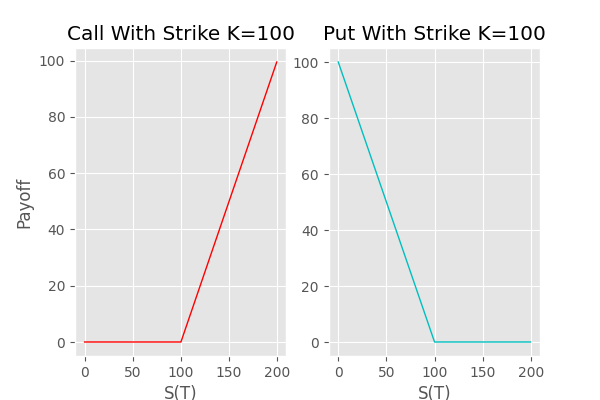
\includegraphics{Figures/contractfct.png}\\
\decoRule
\caption[Contract Functions]{European options payoff at maturity with strike K=100}
\label{fig:contractfct}
\end{figure}

Figure \ref{fig:contractfct} shows that the owner of the option has limited downside, but the graph does not take into account the initial price for the option. The profit and loss ($P\& L$) graph is also a common way of illustrating the payoff for an option, where you take the initial cost of buying the option into account. The European call and American put will be the central derivatives considered together with an American bivariate contingent claim. The task ahead is to find the initial price or the fair price for these contracts, where the concepts of completeness and arbitrage will be central.

%-----------------------------------
%	SUBSECTION 2
%-----------------------------------

\subsection{Self-financing Portfolio (Without Consumption)}
Before being able to use the concepts of arbitrage and completeness, the construction of the portfolio from the financial market model will be important. The portfolio is the number of each assets from the market the owner of the portfolio holds. The value of the portfolio for a market model with the bank account and d stocks is:
\begin{equation*}
V^h(t)=\sum_{i=0}^{d} h_{i}(t) S_i(t)
\end{equation*}
$V^h$ is called the value process and $h_i(t)$ is number of shares of type i during the period "$[t,t+dt)$". For the definition of arbitrage (Definition \ref{Arbitrage}) we need to restrict ourselves to self-financing (S-F) portfolios. A self-financing portfolio h, is a portfolio h which doesn't get any external injection of money.
\theoremstyle{definition}
\begin{definition}{\textbf{Self-financing portfolio: }}
A portfolio consisting of d+1 asset(s): \\
h(t)=($h_0(t),h_1(t), \dotsc, h_{d}$) is self-financing if:
\begin{equation*}\label{SF}
\begin{split}
dV^{h}(t)=\sum_{i=0}^{d} h_{i}(t) dS_{i}(t)
\end{split}
\end{equation*}
Where $S_{i}$ is the $i'th$ asset in our portfolio, d+1 is the total number of assets in our market model and $V^{h}(t)=\sum_{i=0}^{d} h_{i}(t) S_{i}(t)$.\\ \null \hfill (p. 87 \parencite{finKont})
\end{definition}
When dealing with discrete time finance the S-F portfolio is actually a budget restriction, this is important intuition for the continuous time version, because the continuous time version can be thought as the limit of the discrete version by letting step sizes in time tending to zero. To avoid pathological effects on the portfolio one often introduce the concept of an admissible portfolio:
\theoremstyle{definition}
\begin{definition}{\textbf{a-admissible portfolio: }}
For some $a\geq 0$, a portfolio h is called a-admissible if its value process $V^h(t)$ is uniform bounded from below by -a.\\
\null \hfill (p. 139 \parencite{finKont})
\end{definition}
The definition of a-admissible portfolio is to avoid situations as the doubling strategy known from gambling and imposes a limit to the debt arrangement. The important takeaway is that the S-F portfolio is a portfolio where you only reallocate your assets through time within the portfolio.

%-----------------------------------
%	SUBSECTION 3
%-----------------------------------
\subsection{Arbitrage}
Arbitrage is the financial term for a "free lunch". An arbitrage opportunity produces something out of nothing without risk. For a efficient and well function market the "money pumps" cannot exist for long, because the "free lunch" would quickly be eroded by exploitation. In order to avoid making a "money machine" in our market, we want to price derivatives by not introducing arbitrage to the market.  
\theoremstyle{definition}
\begin{definition}{\textbf{Arbitrage: }}\label{Arbitrage}
An arbitrage possibility on a financial market is an admissible self-financed portfolio h such that
\begin{equation*}
\begin{split}
V^{h}(0)=0\\
P(V^{h}(T)\geq 0)=1\\
P(V^{h}(T)>0)>1
\end{split}
\end{equation*}
The financial market $\bm{S}$ is called arbitrage-free if there exist no arbitrage opportunities.\\
\null \hfill (p. 96 \parencite{finKont})
\end{definition}
From the above definition we see that arbitrage is a natural financial requirement for a financial market model, because the investor in a arbitrage portfolio starts with 0 dollars, and without injecting any money, the investor is certain of not losing any money. In addition he has a positive probability by ending up with more than 0 at maturity this cannot be a well function market for both buyers and sellers. To price the derivatives fair in the model, the derivative should not introduce arbitrage to the market. A arbitrage free market is not the only desirable property for the market, we would also like to have a unique price for the derivatives. We can obtain a unique price by replicatation of the derivative cash flow with the other assets in the market model. If every derivative can be replicated the market is complete. 

%-----------------------------------
%	SUBSECTION 4
%-----------------------------------

\subsection{Complete Market And Replication}
The replication argument in Black-Scholes paper \parencite{B-S-Paper} was groundbreaking in the sense that the attitude to risk was irrelevant for pricing, because by continuous trading in the underlying asset(s) the contingent claim cash flow could be replicated. The replication argument shows that the price is unique under the assumption investors prefer more to less. Replication is also important for risk management of the derivative books, because it tells you have to risk neutralize your exposure. A hedge\footnote{Note there is a subtle difference between to hegde or replicate a cash flow. The hedge gives minus the cash flow from replication} is simply a risk neutralization action in order to minimize the overall risk. In the definition below, we define a replication for an simple T-claim\footnote{Options only exercisable at maturity}.
\theoremstyle{definition}
\begin{definition}{\textbf{Replication and completeness for T-claim: }}
A T-claim X can be replicated, if there exist a self-financing portfolio h such that:
\begin{enumerate}
\item[•] $V^{h}(T)=X$ P-a.s.
\end{enumerate}
I.e. h is an replication portfolio for X if it is guaranteed to pay in all circumstances an amount identical to the payout of X.\\
The market is complete, if every derivative in the market can be replicated.\\
\null \hfill (p. 192 \parencite{finKont})
\end{definition}

By introducing the basic concepts for how to price fair and protect ourselves against financial risk, we will in next section focus on building the financial market model.

%----------------------------------------------------------------------------------------
%	SECTION 2
%----------------------------------------------------------------------------------------

\section{Multidimensional Models}\label{MultiDimModel}
There is two main method for deriving arbitrage free and complete markets. The classical approach is the delta hedging approach \parencite{B-S-Paper} and \parencite{CRR}). The more advanced mathematical approach is the martingale approach  \parencite{finKont}. In this section we focus on the martingale approach and show that delta hedging approach coincides with the more general martingale theory. For the martingale approach the First and Second Fundamental Theorems of Mathematical Finance will be the key for obtaining a fair market. Besides the financial market assumptions in section \ref{FinMarket} will we assume specific model assumptions.

\subsection{Model Assumptions}
Let us consider a filtered probability space $(\Omega, \mathcal{F}, P, (\mathcal{F}_t^{\bar{W}})_{t \in [0,T]})$. Note the assumption that filtration is generated from the Wiener process and we consider a finite horizon. We assume $\bar{W}_i$ is k-dimensional and $\bar{W}$ is the only random source. A priori we assume a market $(B(t),S_1(t), S_2(t),\ldots, S_d(t))$, where ${S_i(t)}_{i=1,2,\ldots,d}$ are d risky assets and B(t) is the risk free asset\footnote{B(t) is often also referred to as the bank account}. By assumptions their dynamics are given by:\\
\begin{align}
d\bm{S}(t)&=D[\bm{S}(t)]\bm{\alpha}(t)dt+D[\bm{S}(t)]\bm{\sigma}(t)d\bar{\bm{W}}(t) \quad & S_i(0) &\in \mathbb{R}^+ \label{GBM-P} \\
dB(t)&=r(t)B(t)dt \quad & B(0) &= 1
\end{align}
We assume $\alpha_i(t)$, $\sigma_{ij}(t)$ and the short rate $r(t)$ are adapted processes, this condition are necessary for the stochastic integrals to be well-defined. The evolution of the stocks are described by the geometric brownian motion (GBM) which has a solution to the SDE. The randomness comes from the Wiener process\footnote{A Wiener process is also called a Brownian motion (BM)} in the GBM, which has wildly trajectories. The function $t\mapsto W_{t}(\omega)$ from $[0,\infty)$ to $\mathbb{R}$ is continuous, but nowhere differentiable. Furthermore the BM has nonzero quadratic variation and infinite variation, which is the reason to stochastic calculus pioneered by Itô. The BM has also well-behaved property e.g. it is a Lévy process, i.e. $W(0)=0 \ a.s$, independent and stationary increments $W(t)-W(s)$ which is normally distributed with mean zero and variance t-s. The Brownian motion in the GBM formalizes "random shocks" $dW$ to the stock return with volatility $\bm{\sigma}(t)$ and drift $\bm{\alpha}(t)$. Figure \ref{fig:BM} illustrates three approximations to sample paths of the stocks with GBM assumption with initial value $S_{i}(0)=36$.\\

\begin{figure}[th]
\centering
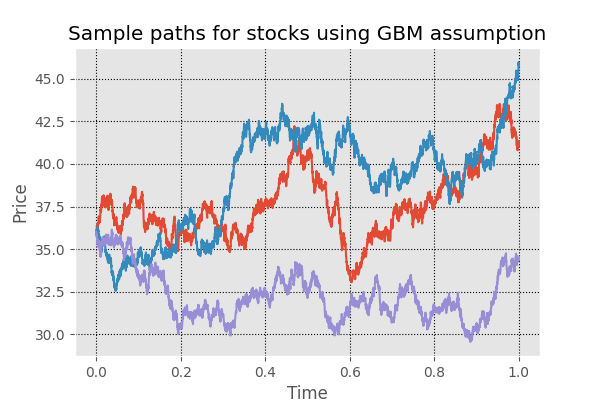
\includegraphics{Figures/samplePath.png}
\decoRule
\caption[Sample Path For Stocks]{Three sample paths for stocks under GBM assumptions, where the spot is \$36, $\sigma$=0.2 and $\alpha$=0.06}
\label{fig:BM}
\end{figure}

The tool for handling BM is stochastic calculus in continuous time, because the standard calculus will not work for the wildly behaved BM. In the representation of the GBM, we used vector and matrix notation for the GBM process. The stock vector is d dimensional and the Wiener process vector is k dimensional. The volatility matrix is given by $\bm{\sigma}(t)=\{\sigma_{ij}(t)\}_{i=1,\ldots,d,j=1,\ldots,k}$ and the drift is $\alpha(t)=(\alpha_1(t), \alpha_2(t), \ldots, \alpha_d(t))^T$. D(x) denotes a diagonal matrix with vector x as its diagonal and the Wiener processes instantaneous correlation matrix $\Sigma$ is given by $Cov(dW_i(t),dW_j(t))=\rho_{ij}dt$.

\subsection{Arbitrage Free Model}
The first problem we are faced with in arbitrage theory is to create a model with no arbitrage opportunities. The First Fundamental Theorem tells us how to not introduce arbitrage to our market model.
\begin{theorem}\label{FFT1}
\textbf{First Fundamental Pricing Theorem of Mathematical Finance(FFT1): } The market model is free of arbitrage if and only if there exist a equivalent martingale measure, i.e. a measure $Q\sim P$ such that the processes:
$$\frac{S_0(t)}{S_0(t)}, \frac{S_1(t)}{S_0(t)}, \cdots, \frac{S_d(t)}{S_0(t)}$$
are (local)martingales under Q.
\\ \null \hfill (p. 154 \parencite{finKont})
\end{theorem}
The processes are martingales is a mathematical formulation that the expected value of the discounted value coincides with the known spot value today\footnote{Assuming $B(0)=1$}. In gambling a martingale resembles a "fair" game. From the FFT1 using the bank account $B(t)$ as numéraire it follows that:
\theoremstyle{proposition}
\begin{proposition}{}
We assume that $B(t)=S_0(t)$ is our numéraire and all the processes randomness comes from the Weiner process, then a equivalent measure $Q \sim P$ is martingale measure if and only if all assets $(B(t), S_1(t), \ldots, S_d(t))$ have the short rate as their local rates of return, i.e.
\begin{align*}
dS_i(t)=S_i(t)r(t)dt+S_i(t)\sigma_i(t)dW^Q(t)
\end{align*}
\null \hfill (p. 154 \parencite{finKont})
\end{proposition}
So to not introduce arbitrage to the model for the financial market, we need to ensure the Q-dynamics of S is:
\begin{equation}\label{Q-dym}
dS(t)=D[S(t)]r(t)dt+D[S(t)]\sigma(t)d{W}(t)
\end{equation}
The tool to obtain the dynamics in equation \eqref{Q-dym} is Girsanov theorem (theorem \ref{Girsanov}). Girsanov theorem is a continuous measure transformation, where in our model we want to transform the dynamics given with the objective probability measure P to an equivalent martingale measure Q. By suitable chooses of the likelihood process L and setting $dQ=L(T)dP$, then with Girsanov theorem the transformed process is still a Brownian motion:
$$d\bar{W}(t)=\phi(t)dt + dW(t)$$
When applying to eq. (\ref{GBM-P}):
$$dS(t)=D[S(t)](\alpha(t)+\sigma(t)\phi(t))dt+D[S(t)]\sigma(t)d{W}(t)$$
Going back to the FFT1 and the proposition hereof, we know that Q is martingale measure if and only if:
\begin{align}\label{marketPriceOfRisk}
\bm{\alpha}(t)+\bm{\sigma}(t)\bm{\phi}(t)=\textbf{r}(t) \quad holds \ with \ probability \ 1 \ for \ each \ t
\end{align}
We disregard pathological models when doing so the term generically arbitrage free will be used. 

\theoremstyle{definition}
\begin{definition}{\textbf{Generically arbitrage free}:}
The model in this section is said to be generically arbitrage free if it is arbitrage free for every (sufficiently integrable) choice of $\bm{\alpha}(t)$.
\\ \null \hfill (p. 198 \parencite{finKont})
\end{definition}

Furthermore we assume enough integrability and we have the following useful result:
\theoremstyle{proposition}
\begin{proposition}{}\label{arbitrageFreeProp}
Disregarding integrability problems the model is generically arbitrage free if and only if, for each $t\leq T$ and P-a.s. the mapping:
$\bm{\sigma}(t):\mathbb{R}^k \to \mathbb{R}^d$ is surjective, i.e. if and only if the volatility matrix $\bm{\sigma}(t)$ has rank d.
\\ \null \hfill(p. 198 \parencite{finKont})
\end{proposition}
We note that in order not to have arbitrage in our model, we need $k\geq d$, i.e. have at least as many random sources as number of risky assets.

\subsection{Complete model}
Second Fundamental Pricing Theorem is key to obtain a complete market model, i.e. a market model with unique prices and every claim can be hedged.
\begin{theorem}\label{FFT2}
\textbf{Second Fundamental Pricing Theorem of Mathematical Finance(FFT2): } Assuming absence of arbitrage, the market model is complete if and only if the martingale measure $Q$ is unique.
\\ \null \hfill (p. 155 \parencite{finKont})
\end{theorem}
In our Wiener world we have a unique martingale measure if equation \ref{marketPriceOfRisk} has a unique solution. The proof of proposition \ref{completeProp} will shortly reveal why the Wiener world assumption is required. If we had more random sources e.g. a Poisson process\footnote{The Merton's Mixed Jump-Diffusion Model is an example}, than there is no guarantee that the equivalent measure transformation is of the Girsanov type above. 

\begin{proposition}{}\label{completeProp}
Assume that the model is generically arbitrage free and that the filtration is defined by:
$$\mathcal{F}_t=\mathcal{F}_t^{\bar{W}} \quad t \in [0,T]$$
Then disregarding integrability problems, the model is complete if and only if k=d and the volatility matrix $\sigma(t)$ is invertible P-a.s. for each $t \leq T$
\begin{proof}
The proof is based on martingale representation theorem \ref{MRT} (MRT) and converse of Girsanov theorem \ref{ConverseGirsanov} which uses MRT, hence the assumption about the only randomness comes from the Wiener process. By the two theorems we know every equivalent measure transformation is obtained by Girsanov theorem of the above type. Hence the martingale measure is unique if and only if the solution to \eqref{marketPriceOfRisk} is unique.                                        
\end{proof}
\null \hfill (p. 200 \parencite{finKont})
\end{proposition}
Intuitively we need one independent traded assets excluding the bank account for every source of randomness (Meta-theorem 8.3.1 \parencite{finKont}).


\subsection{Pricing and Connection to Classical Approach}
The pricing formula for arbitrage free market model is the risk neutral valuation formula(RVNF):
\begin{proposition}{\textbf{Risk Neutral Valuation Formula}}\label{RNVF}
To avoid arbitrage, $\mathcal{X}$ must be priced according to the formula:
\begin{align}
\Pi(t;\mathcal{X})=S_0(t)E^Q[\frac{\mathcal{X}}{S_0(T)}|\mathcal{F}_t]
\end{align}
Note if we choose our numéraire $S_0(t)=B(t)$ then
\begin{align}
\Pi(t;\mathcal{X})=E^Q[\exp(-\int_t^T r(s) ds) \mathcal{X}|\mathcal{F}_t]
\end{align}
\null \hfill(p. 155 \parencite{finKont})
\end{proposition}
Proposition \ref{RNVF} will raise the question if there is more than one fair price for the derivative. The answer is found in FTT2, the market is complete if and only if the measure Q is unique. Intuitively it means that if you can replicate the derivative with a S-F portfolio, then the risk free position should only earn risk free interest rate. The conditional expectation in the RNVF is a natural choice for pricing, because intuitively the conditional expectation is our best estimate given the available information\footnote{Mathematically known as the projection property}.\\

The classical approach in \parencite{B-S-Paper} to arbitrage free and complete market models is based on a Markovian model assumption. For the model to have the Markov property, we assume $k=d$ and the probability space is $(\Omega, \mathcal{F}, P, \mathcal{F}_t^{\bar{W}_t})$. Furthermore we assume $\bm{\alpha}$ and $\bm{\sigma}$ are deterministic and constant over time. $\bm{\sigma}$ is also assumed invertible. Under these more restrictive assumptions the risk neutral valuation formula for a simple T-claim is given by the pricing function:
\begin{align}\label{MarkovRNVF}
F(t,S(t))=\exp(-r(T-t))E^Q[\mathcal{X}|S(t)]
\end{align}
The Markov property implies that the price only depend on the current state of $\bm{S}$. Applying Kolmogorov backward equation on equation \eqref{MarkovRNVF} we obtain the Black-Scholes PDE for the pricing function $F(t,S(t))=\Pi(t; \mathcal{X})$.

\begin{theorem}\label{BSPDEMultiDim}
\textbf{Black Scholes PDE: } Consider the contract $\mathcal{X}=\Phi(\bm{S}(T))$. In order not to introduce arbitrage to the market, the pricing function $F(t,s)$ must solve the boundary value problem.
\begin{equation*}
\begin{split}
F_t(t,s)+\sum_{i=1}^{n} rs_iF_i(t,s)+\frac{1}{2} tr\{\sigma^* D[S] F_{ss} D[S] \sigma\} -rF(t,s)&=0\\
F(T,s)&=\Phi(s)
\end{split}
\end{equation*}
\null \hfill (p. 203 \parencite{finKont})
\end{theorem}


%----------------------------------------------------------------------------------------
%	SECTION 3
%----------------------------------------------------------------------------------------
\section{Classical Black-Scholes Theory}\label{classicBS}
We will not do the classical delta hedging approach in \parencite{B-S-Paper}. Instead we use the general multidimensional martingale approach to derive the essential formulas for pricing. 
To derive a closed-form solution to the European call and put option, we concentrate at a special case of the multidimensional framework, where we only have the risk free asset and one risky asset in the financial market model. 
We further restrict ourselves to:
\theoremstyle{assumption}
\begin{assumption}{\textbf{Black-Scholes assumptions}:}\label{BS-Assumption}
We assume following ideal conditions in addition to \eqref{EfficientMarket}:
\begin{enumerate}
\item[•] The short-term interest rate $r\in \mathbb{R}^+_*$\footnote{Note that restricting the interest rate to the positive reals is not part of the Black-Scholes papers assumptions.}, volatility $\sigma \in \mathbb{R}^+$ and the drift $\alpha\in \mathbb{R}$ are constant.
\item[•] The stock pays no dividends or other distributions.
\item[•] The option is a simple option ("European").
\item[•] No arbitrage opportunity on the market.
\end{enumerate}
\null \hfill (p. 640 \parencite{B-S-Paper})
\end{assumption}
The interest rate is assumed strictly positive to assure the European call and American call value coincides\footnote{Detailed explained in section \ref{AmericanCall}}. The above assumptions gives the Markovian model described in previous section. \\

We assume the underlying stock and the bank account have differentials:
\begin{align*}
dS(t)&=S(t)\cdot \alpha dt+S(t) \sigma d\bar{W}(t) \quad & S(0) &\in \mathbb{R}^+ \\
dB(t)&=r B(t)dt \quad & B(0) &= 1
\end{align*}
By Itô's lemma (lemma \ref{Ito}) for one dimensional process the solution to the differentials above is:
\begin{align*}
S(t)&=S(0) \cdot \exp \bigg( (\alpha -\frac{1}{2} \sigma^2) t + \sigma W(t) \bigg) \\
B(t)&=\exp(r\cdot t)
\end{align*}
The solution of the SDE of S under Q dynamics is:
\begin{equation}\label{GBM}
\begin{split}
S(t)=S(0) \cdot \exp \bigg( (r -\frac{1}{2} \sigma^2) t + \sigma W(t) \bigg)
\end{split}
\end{equation}
By equation \eqref{GBM} we see that the Black-Scholes model assumes that the stock price evolution produces a lognormal distribution for the price at any future time. \\

The closed form solution for the European call can be derived solving the Black-Scholes PDE or with the RNVF given in previous section. 
\theoremstyle{proposition}
\begin{proposition}{}\label{BS-price-EuroCall}
\textbf{Black-Scholes formula for call option: } The price of a European call option with strike K and maturity T is given by the formula  $\Pi(t)=F(t,S(t)$, where
\begin{align*}
F(t,s)=c(t,s)=s \cdot N(d_1(t,s)) - e^{-r(T-t)}\cdot K \cdot N(d_2(t,s))
\end{align*}
N is the cumulative distribution function of a standard normal distribution $\mathcal{N}(0,1)$ and
\begin{align*}
d_1(t,s)=\frac{1}{\sigma\cdot \sqrt{T-t}} \cdot \bigg( \ln(\frac{s}{K}) + (r+\frac{1}{2} \sigma^2) (T-t) \bigg)\\
d_2(t,s)=d_1(s,t)-\sigma \sqrt{T-t}
\end{align*}
\null \hfill (p. 105 \parencite{finKont})
\end{proposition}
We provided only the price for the European call option, but the European put price can readily be obtained by the put-call-parity for European options.

\theoremstyle{proposition}
\begin{proposition}{}\label{put-call-parity}
\textbf{Put-call parity: } 
Assume the call and put option has same strike price and time to maturity.
\begin{align*}
p(t,s)=K\cdot \exp(-r(T-t))+c(t,s)-s
\end{align*}
\null \hfill (p. 126 \parencite{finKont})
\end{proposition}

The aim for this thesis is to price American put options, but the European option provide a reference price in a closed form format. The put-call-parity holds only for European options, where for the American option there is a bound on the difference in price:
$$S_0 - K \leq C-P \leq S_0 - K \cdot e^{-rT}$$

The above formula for the European call option is actually the same for an American call option, but is not true for an American put option or for call options with underlying stock paying dividends. The result for the American call option was shown by Merton \parencite{Merton73}, that the intrinsic value is never greater than the worth of the option given by the risk-neutral valuation formula. In section \ref{AmericanOptions} we will show a martingale approach to prove the value of a European and American call coincides when the underlying is a non-dividend paying stock.

%----------------------------------------------------------------------------------------
%	SECTION 4
%----------------------------------------------------------------------------------------

\section{American Options And Optimal Stopping}\label{AmericanOptions}
The American options adds additional complexity to the pricing problem, because compared to the European option the American option can be exercised at anytime from inception to maturity. The exercise value at time t is also called the intrinsic value of the option. This section is inspired by \parencite{finKont, Shiryaev06,Elliott99} where \parencite{Shiryaev06} is specialized to optimal stopping problems and the two other references give the fundamentals for option and arbitrage theory in general.\\

We still assume a diffusion setting that the underlying stochastic process for the stock behaves under the risk neutral measure as a GBM. The exercise feature of the American option raises the problem of rationally to find the optimal stopping time to maximize profit. The value of the option is given by exercising the option at the optimal stopping time, hence it is a optimal stopping problem. We will assume a finite horizon $T\in \mathbb{R}_*^+$ throughout the thesis, because all the derivative will be priced in a finite timeframe. Let the gain function $G:\mathbb{R}\to \mathbb{R}$ be a measurable function satisfying:
\begin{equation}\label{existAmer}
E_{s}[\sup_{0\leq t \leq T}|G(S(t))|] < \infty
\end{equation}
where $S$ is the underlying stochastic process. If the integrability condition is satisfied on a finite interval $[0,T]$ (equation \eqref{existAmer}) then the optimal stopping problem for gain function G and $s \in \mathbb{R}$ is well defined. We assumed that the underlying stochastic S(t) process is time-homogeneous, but the assumption can be relaxed. If S(t) is a time-inhomegenous we can extend the underlying process S(t) by time albeit increasing the underlying process dimension. We define the optimal value process in terms of the gain process.

\theoremstyle{definition}
\begin{definition}{}\label{optValFunc}
For fixed $(t,x)\in [0,T] \times \mathbb{R}$, and each stopping time $\tau$ with $\tau\geq t$ the optimal value function $V(t,x)$ is defined by
\begin{align}
V(t,x)= \sup_{\tau \in \mathcal{T}^T} E_{t,x}[G(S(\tau))]
\end{align}
A stopping time which realizes supremum for V is called optimal and be denoted $\hat{\tau}$.
\\ \null \hfill (p. 341 \parencite{finKont})
\end{definition}

The solution to the optimal stopping problem $\hat{\tau}$ is where supremum is attained and the price is then $V(t,x)$ for $(t,x)\in [0,T] \times \mathbb{R}$. The supremum is taken over all stopping times with respect to the natural filtration $\mathcal{F}_{t}$ belonging in the class of stopping times:
$$\mathcal{T}_0^T=\mathcal{T}^T=\{\tau : 0 \leq \tau \leq T \}$$
The definition of a stopping time $\tau$ can be seen in definition \ref{StoppingTime}. The intuition is that the stopping time is a random time, where we know at present time weather the process is stopped or not. To solve the optimal stopping problem some trivial solutions are immediate by martingale properties:
\begin{proposition}\label{TrivialMG}
The following hold:
\begin{enumerate}
\item[•] If $G(S(t))$ is a submartingale, then it is not optimal to stop at all and $\tau^*=T$
\item[•] If $G(S(t))$ is a martingale, then all stopping times $\tau\in [0,T]$ are optimal
\item[•] If $G(S(t))$ is a supermartingale, then it is optimal to stop immediately. i.e. $\tau^*=0$
\end{enumerate}
\null \hfill(p. 330 \parencite{finKont})
\end{proposition}

Examples of optimal stopping problems could be the American call and put options:
\begin{align*}
C(t,x)=\sup_{\tau \in \mathcal{T}_t^T} E^Q[\exp(-r(\tau-t)) (S(\tau)-K)^+|S(t)=x] \quad for \ t\in [0,T] \ and \ x\in\mathbb{R}^+\\
P(t,x)=\sup_{\tau \in \mathcal{T}_t^T} E^Q[\exp(-r(\tau-t)) (K-S(\tau))^+|S(t)=x] \quad for \ t\in [0,T] \ and \ x\in\mathbb{R}^+
\end{align*}


\subsection{American Call Without Dividends}\label{AmericanCall}
The American call options is a special case, because the optimal stopping time is always at the options maturity. With martingale machinery it means the value-process is a submartingale which implies that $\hat{\tau}=T$ (proposition \ref{TrivialMG}). Remember the optimal stopping problem for an american call option:
$$C(t,x)=\sup_{\tau \in \mathcal{T}_0^{T-t}} E_{t,x}^Q[\exp(-r\tau) (S(t+\tau)-K)^+]$$
Looking at the gain function:
\begin{equation*}
\exp(-r t) (S(t)-K)^+ = (\exp(-r t) S_{t} - \exp(-r t) K)^+
\end{equation*}
Recall that the discounted price process $\exp(-r\cdot t) \cdot S_t$ is a Q-martingale and $\exp(-r\cdot t) \cdot K$ is a deterministic decreasing function in t if $r>0$. Furthermore the function $x \mapsto (x)^+$ is convex, hence the gain function is a $Q$-submartingale. The last result used is that a convex and increasing function on a submartingale is still a submartingale, hence the optimal stopping time is $\hat{\tau}=T$ if $r>0$.

\subsection{American Put}\label{americanPut}
The arbitrage-free price for an American put at time t:
\begin{equation}\label{AmericanPutPrice}
P(x,t)=\sup_{\tau \in \mathcal{T}_t^T} E^Q[\exp(-r(\tau-t)) (K-S(\tau))^+|S(t)=x] \quad for \ t\in [0,T] \ and \ x\in\mathbb{R}^+
\end{equation}
For the American put we need computational methods, because the American and European put does not coincides like for the call option.

\begin{proposition}{}
Consider European and American put options with same maturity T and strike K. If the risk free rate $r\in \mathbb{R}_*^+$, then for any $t<T$
\begin{equation}
\begin{split}
p(x,t)<P(x,t)
\end{split}
\end{equation}
\begin{proof}
WLOG\footnote{Without loss of generality} we assume that t=0. Define the stopping time
$$\tau = min \{t\geq 0 : S(t) \leq K(1-\exp(-r\cdot (T-t)))\}$$
We consider a exercise strategy $min\{\tau, T\}$, where the strategy is not necessarily optimal. We consider two events:
\begin{enumerate}
\item[1)] $\tau<T$
\item[2)] $\tau \geq T$
\end{enumerate}
The first case is to exercise at time $\tau$ when $S(\tau) \leq K(1-\exp(-r\cdot (T-t)))$. Here the payoff by exercising will be at least $K\exp(-r\cdot (T-\tau))$. The cash flow received is then invested into the bank account at time $\tau$. At maturity the strategy gives the holder of the put a payoff K, where the European contract with strike K will pay less, because the stock price at maturity will be $S(T)>0 \ a.s.$
The second case is trivial, because the European and American put will give the same payoff. \\
Since the first case has positive probability, the American put has higher discounted expected payoff by following above strategy regardless of the spot price for the stock. 
\end{proof}
\end{proposition}
The above proposition shows the optimal stopping strategy is not always to hold the option to maturity, hence the theory of optimal stopping is important for pricing of American put options. The American put has consequently no closed form solution, but we can search for a lower exercise boundary b(t) such that the holder of the option should exercise when:
$$S(\tau)\leq b(\tau) \quad \tau \leq T$$
The continuation set $C$ and stopping set $\bar{D}$ are given for an American put.
\begin{align*}
C=\{(t,x) \in [0,T) \times (0,\infty) : V(t,x) > G(x) \}\\
\bar{D}=\{(t,x) \in [0,T) \times (0,\infty) : V(t,x) = G(x) \}
\end{align*} 

Hence the first optimal stopping time after time t for the American put is
\begin{equation*}
\begin{split}
\hat{\tau}= \inf\{u \in [t,T] : P(S(u),u) = (K-S(u))^+ \}
\end{split}
\end{equation*}

\subsection{Discrete time valuation}\label{DiscreteValueFramework}
To solve the optimal stopping problem numerical methods are required for the American put option, hence the first step is to discretize exercise dates. In chapter \ref{Chapter3} we show two approaches to price an American put option, where both are based on calculating the expected continuation value. \\

Suppose the probability space $(\Omega, \mathcal{F}, P)$ is equipped with the natural discrete filtration $(\mathcal{F}_{t_n})_{n=0,1,\ldots,N}$ modeling a financial market. By discretization of time we are actually looking at a Bermudan option, but for sufficient small time steps the Bermudan option approximate the American option well. The tenor structure\footnote{The tenor of an option is the remaining life of the option from today to maturity} is that the time to maturity is divided into a grid of N+1 equidistant points in time $0=t_0\leq t_1\leq t_2, \cdots \leq t_N=T$, where $\Delta t_n = t_n-t_{n-1}=T/N$ for each $n=1, \ldots, N$. A Bermudan option initialized at time $t_0$ has $\mathcal{T}(t_0,t_1,\ldots,t_N)$ exercise dates or decision points, where the option holder chooses to exercise or keep the option alive. \\

The underlying process is assumed to be Markovian with state variables $(S(t_n))_{n=0,1,\ldots,N}$ recording all necessary information about relevant financial variables adapted to the natural filtration in order to solve the optimal stopping problem with the dynamic programming principle. Furthermore is the gain process adapted to the filtration and square integrable $E[\max_{0\leq n \leq N} |G(S(t_n))|^2]<\infty$, which is necessary to use regression on a finite set of functions to approximate the conditional expectation (section \ref{LSM}).\\

The optimal stopping problem in discrete time is to find
\begin{equation}\label{Bermudanstop1}
\sup_{\tau \in \mathcal{T}(0,1,\ldots,T)} E^Q[G(S(\tau))]
\end{equation}
For using the programmable dynamic programming principle the Snell envelope $(U(t_{n}))_{n=0,1,\ldots, N}$ (definition \ref{snellEnvelope}) of the gain function $G(S(t_n))_{n=0,\ldots,N}$ is useful and defined by
$$U(t_n)=\esssup_{\tau \in \mathcal{T}(n,\ldots, N)} E^Q[G(S(\tau_{t_n}))|S(t_n)] \quad n=0,1, \ldots, N$$
The Snell envelope $U(t_n)$ is the smallest supermartingale of the gain process $\{G(S(t_n))\}$, i.e. the smallest supermartingale dominating the gain process. Using the Snell envelope theory the optimal stopping problem can be solved with the dynamic programming principle.
\begin{equation}\label{valueIteration}
\begin{split}
\begin{cases}
          U(t_{N}) = G(S(t_N))\\
          U(t_n) = max\{ G(S(t_n)), E^Q[U(t_{n+1})|S(t_n)])\} \quad for \ n={0,\ldots,N-1} \\ 
\end{cases}
\end{split}
\end{equation}
Where $U(t_n)$ is the discounted option value at time $t_n$ not previous exercised and $G(S(t_n))$ is the discounted exercise value.\\

Equation \eqref{valueIteration} is known as value iteration indicates that the holder should exercise the first time $G(S(t_n))> E^Q[U(t_{n+1})|S(t_n)])$ in order to maximize payoff from the option, hence we get the first optimal stopping time. Note that an optimal stopping time will always exist in discrete time when $T<\infty$. There is though no guarantee that the stopping time is unique. The value iteration gives the optimal value process of the gain process $G(S(t))$ (theorem \ref{SnellEnvelopeTheorem}). So 
$$U(t_n)=E^Q[G(S(\tau_{t_n})|S(t_n)]$$ with 
$$\tau_{t_n}=\min \{ k \geq n : U(t_k) = G(S(t_k)) \}$$ and 
$$E^Q[U(0)]= \sup_{\tau \in \mathcal{T}(0,\ldots, T)} E^Q[G(S(\tau))]=E^Q[G(S(\hat{\tau}))]$$ 
The optimal stopping problem can also be solved in terms of stopping times instead of using the value process. This alternative dynamic programming principle equation is called policy iteration.
\begin{equation}\label{policyIteration}
\begin{split}
\begin{cases}
          \tau_{t_N} = t_N\\
          \tau_{t_n} = t_n \cdot 1_{\{G(S(t_n)) \geq E^Q[G(\tau_{t_{n+1}})|S(t_n)])\}} + \tau_{t_{n+1}} \cdot 1_{\{G(S(t_n)) < E^Q[G(\tau_{t_{n+1}})|S(t_n)])\}} \quad for \ n={0,\ldots,N-1} \\ 
\end{cases}
\end{split}
\end{equation}

The first approach in chapter \ref{Chapter3}, the binomial model, uses the idea of dynamic programming. The underlying stochastic process is approximated by a discrete binomial recombining tree, which is readily to work backward in time to calculate both European and American option prices. The American put option can be solved recursively with dynamic programming principle with value iteration: 
\begin{equation}\label{BellmanEq}
\begin{split}
\begin{cases}
          P(t_i) = max\{ (K-S(t_i))^+, \exp(-r\cdot \Delta t) E^Q[P(t_{i+1})|S(t_i)\} \quad for \ i={0,\ldots,N-1} \\
          P(t_N) = (K-S(t_N))^+ 
\end{cases}
\end{split}
\end{equation}

The second approach, Least Square Monte Carlo Method (LSM) model, is to combine dynamic programming and Monte Carlo simulation, but this method uses the policy iteration principle instead of the value iteration. The method uses regression to calculate the expected continuation value of simulated paths instead of discretization of the underlying stochastic process. LSM overcomes the challenge with pure simulation method by using regression, because it gives an effective way to evaluate a series of conditional expectations. Both methods will be explained in details in chapter \ref{Chapter3}.





  

\chapter{Classical numerical results and Benchmarks} % Main chapter title

\label{Chapter3} % Change X to a consecutive number; for referencing this chapter elsewhere, use \ref{ChapterX}

In last section we saw that the american put was an example of an option that required numerical procedures to be priced fair. The American put is far from the only example of a derivative without a closed-form solution. We will look at two classical valuation algorithms for pricing american options in computational finance the Cox-Ross-Rubinstein (CRR) binomial model \parencite{CRR} and the Least Square Monte Carlo (LSM \parencite{lsm}). The binomial model is an example of a strategy to approximate the american option by discretization of the underlying risky asset(s) and the LSM is a method to simulate the underlying risky asset(s). Another popular choice is to solve the free boundary problem with finite difference methods, but we chose to focus on the two other numerical procedures. The chapter will also investigate valuing exotic multivariate contingent cliams. We extend the binomial pricing model (\parencite{NEK,BEG}) and LSM to multivariate contingent claims and provide some closed form solutions for exotic european options (\parencite{Johnson87, Ouwehand2006}). We wrap up the chapter with numerical findings. Therefore the chapter have two purposes to gain insight into valuation for exotic options and provide some benchmarks for the Neural Network in the coming chapters.

%----------------------------------------------------------------------------------------
%	SECTION 1
%----------------------------------------------------------------------------------------
\section{Cox Ross Rubenstein Model}\label{CRR}
The classical binomial model pricing formula or the CRR model presented in this section is inspired by \parencite{CRR,Hull,finKont}. The model will be used for pricing an american put option with 1 underlying stock and to build the foundation for pricing bivariate contingent claims with the binomial model \parencite{BEG}. The CRR model provides an intuitive and easy implementable model for valuing american and european options. The binomial model comes handy, when no analytical model exists e.g. for an american put option. The Binomial model also has its limitations, because for computational reasons it is not suited for valuing path dependent options or options with several underlying factors. The key difference on the binomial model and the simulation approach is that the binomial model discretize the underlying stochastic process(es) in time. \\

Assume the same market and Black-Scholes assumptions as in chapter 2, but the underlying stochastic process will be assumed to follow a multiplicative binomial process over discrete periods. We work with the financial market $(\Omega, \mathcal{F}, \mathbb{F}, P, S_0, S_1)$, where the filtration is generated by $\mathbb{F}= \sigma(\mathcal{F}_{t_n})_{n=0,1,\ldots, N}$ and the sigma algebra is chosen to be $\mathcal{F}=\mathcal{F}_{t_{N}}$. It is well known from discrete arbitrage teory, that the binomial market model with two assets, where $u>1+r>d>0$ is a complete and arbitrage free model. The u,d and r describes the evolution of the discrete stochastic process for the stock and the free interest rate on the bank account. 
\begin{align*}
S_{0}(t_n)=S_{0}(t_{n-1}) \cdot \exp(\Delta t \cdot r) \quad where \ S_{0}(0)=1 \ and \ n=0, \ldots, N\\
S_{1}(t_n)=S_{1}(0)\prod_{j=1}^{n} Y_{j} \quad where \ Y_1,Y_2, \ldots, Y_N \ are \ i.i.d., \ S_1(0)>0
\end{align*}
Note that the interest rate is continuously compounded for computational convience and the equidistant time step is $\Delta t=T/N$ (section \ref{DiscreteValueFramework} for notation). We assume that \[ Y_i = \begin{cases} 
      u & with \ probability \ p \\
      d & with \ probability \ (1-p)
   \end{cases}
\]

Below a illustration of a discrete multiplicative binomial process with two time steps, where the lattice recombines.

\begin{figure}[H]
\centering
% Define styles for bags and leafs
\tikzstyle{bag} = [text width=2em, text centered]
\tikzstyle{end} = []
\begin{tikzpicture}[sloped]
   \node (a) at ( 0,0) [bag] {$S(0)$};
   \node (b) at ( 4,-1.5) [bag] {$d S(0)$};
   \node (c) at ( 4,1.5) [bag] {$u S(0)$};
   \node (d) at ( 8,-3) [bag] {$d^2 S(0)$};
   \node (e) at ( 8,0) [bag] {$d u S(0)$};
   \node (f) at ( 8,3) [bag] {$u^2 S(0)$};
   \draw [->] (a) to node [below] {$(1-p)$} (b);
   \draw [->] (a) to node [above] {$p$} (c);
   \draw [->] (c) to node [above] {$p^2$} (f);
   \draw [->] (c) to node [above] {$(1-p)p$} (e);
   \draw [->] (b) to node [below] {$(1-p)p$} (e);
   \draw [->] (b) to node [below] {$(1-p)^2$} (d);
\end{tikzpicture}
\decoRule
\caption[Two Dimensionel Binomial Lattice]{Price dynamics of binomial model with one underlying risky asset with N=2, $S(0)$ is spot value, p objective probability measure, u and d is realizations of the stochastic variable $Y_i$}
\label{fig:twoDimLattice}
\end{figure}

By construting the discrete process for the stock it is easy to find the equivalent martingale measure. 
\begin{definition}\label{findQ}
Assume there exists a risk free asset. A probability measure $Q$ is called a martingale measure if the following condition holds 
\begin{align}
s= \exp(- r \Delta t) \cdot E^Q[S(t+\Delta t)|S(t)=s] 
\end{align}
Where $\Delta t$ is a single time-step (p. 18 \parencite{Bjork19}).
\end{definition}
By using definition \ref{findQ} we find the risk neutral measure to be:
$$q=\frac{e^{r \Delta t}-d}{u-d}$$
The martingale measure q is unique in the binomial model, because the model is complete. By above assumption about $u>1+r>d>0$ the binomial model with the market ($S_0(t_n), S_1(t_n)$) is a arbitrage free and complete model, hence to the general pricing formula is given by the risk neutral valuation formula.
\begin{theorem}\label{RNVF-Discrete}
\textbf{Risk-neutral valuation formula (RVNF) in discrete time for T-claim}
The arbitrage free price at t=0 of a T-claim $X$ is given by
\begin{align}
\Pi(0;X)&= \exp(- r \Delta t \cdot N) \cdot E^Q[X]\\
&=\exp(- r \Delta t \cdot N) \cdot \sum_{n=0}^{N} \binom{N}{n} q^n (1-q)^{N-n} \Phi(su^n d^{N-n})
\end{align}
here $Q$ denotes the martingale measure, $\Pi(0;X)$ is the price of X to time 0 and $\Delta t$ is a single time step (p. 25 \parencite{Bjork19}).
\end{theorem}

By above formula the binomial model gives a simple mathematical framework for pricing european options, but the model can easily be extended to american options. American put options for the binomial will be solve with the dynamic programming approach, because the binomial model gives a recursive formula where the one-step transition probabilities are the same in each node.
\begin{equation}\label{BellmanEq2}
\begin{split}
\begin{cases}
          P(t_i) = max\{ (K-S(t_i))^+, \exp(-r\cdot \Delta t) E^Q[P(t_{i+1})|S(t_i)])\} \quad for \ i={0,\ldots,N-1} \\
          P(t_N) = (K-S(t_N))^+ 
\end{cases}
\end{split}
\end{equation}
The idea is to at each decision point either exercise to gain the intrinsic value or hold the option alive for another period. The value of keeping the option alive is called the expected continuation value and it is given by the risk neutral valuation formula. The dynamic choice to exercise or to keep the option alive gives a exercise barrier $b$ (see section \ref{americanPut}).\\

So to value an American put option, we lay out all the possible path of the stock based on $S_1(0),\sigma$ and $T$. These paths construct the tree, then for valuation we work backwards in the tree starting at maturity. Figure \ref{fig:BinomialTree} is an example of a constructed tree, where the value of the option is also included by color. The decision to exercise is marked with a triangle where the decision points where is optimal to keep the option alive is marked with circles. \\

\begin{figure}[th]
\centering
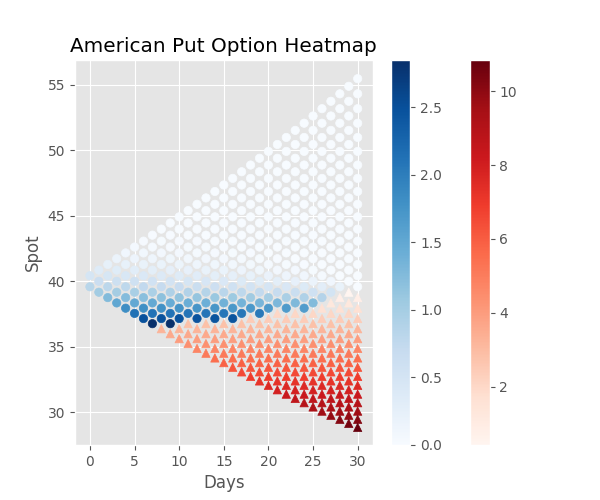
\includegraphics{Figures/BinomialTree.png}
\decoRule
\caption[Binomial Tree]{A valuation tree of an american put option price based on the binomial model, where the color indicate the value and the dots are marking the continuation nodes. The parameters are S(0)=40, N=30, $\Delta t =$ 1 day, K=40 and u=1.0106}
\label{fig:BinomialTree}
\end{figure}

To construct the tree we need to specify the number of equidistant time-steps $\Delta t$ ($\Delta t = \frac{T}{N} \ where \ N=No. \ of  \ steps$) for the tree, where for each step we add another possible value for the stock. We only add 1 more possibility for each time-step because the tree recombines \footnote{$(1+n)$ possible stock values after n steps}. The d and u is chosen such that they match volatility.
$$u= \exp(\sigma \sqrt{\Delta t}) \quad d= \exp(-\sigma \sqrt{\Delta t})$$
For valuing an American put option, we value the exercise value at maturity (time T) for all possible outcomes for the price process at maturity. Then we use backward induction/dynamic programming where we compare the intrinsic value with the expected continuation value (see \eqref{BellmanEq2}), where we choose the maximum of these two. The comparison will be applied for every node in each decision point $(t_{n})_{n=0,1,\ldots,N-1}$ and all the way back in time to the initialization date. By this procedure we get present value of the American option. One design decision is to choose number of time-steps considering a trade-off between computational efficientcy and accurary. Figure \ref{fig:binConv} illustrates that around 40 steps the option value stabilizes for an option with 1 year to maturity. The precision for the algorithm increases with the number of steps and the option value stabilizes for increasing number of steps (see Figure \ref{fig:binConv}).\\

\begin{figure}[th]
\centering
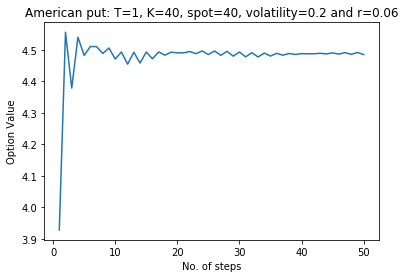
\includegraphics{Figures/binConv.png}
\decoRule
\caption[Convergence Of Binomial Model]{Price for a american put option based on the binomial model, where the independent variable is the number of time-steps. Vol. is an abbreviation for volatility.}
\label{fig:binConv}
\end{figure}

We have seen the central concepts arbitrage and completeness from continuous time in action for the discrete time setup. The paper \parencite{CRR} which introduced the binomial model to option pricing came after the Black-Scholes model described in section \ref{Chapter2} \parencite{B-S-Paper}. The main reason for developing a model in discrete time is that the discrete time approach gives a simplified model in terms of the mathematics and highlights the essential concepts in arbitrage theory. You can argue that the simpler mathematics in this model makes the binomial model more instructive and clear. Besides being easier to understand for non-mathematician it works nicely with other options than the european options like american options. Even though we assume the stock price moves at discrete jumps instead of the classical Black-Scholes continuous time model, it can actually be shown that the CRR binomial model will converge to the continuous time model. Hence the binomial pricing model will be equivalent with the continuous time analytical pricing model derived by Fischer Black and Myron Scholes in the limit for european options for sufficient small time steps. \\

Note for computational resources the path-independence payoff for the american put makes the tree recombining is important, so there is only N+1 terminal nodes at maturity. If the derivative was path-dependent e.g. an asian option, then we have a non-recombinin tree and $2^{N}$ terminal nodes where needed. This is a computational inefficient, which explains that the binomial model should not be used for path-depending derivatives. The problem with a derivative with several underlying e.g. a basket option is also the increasing number of nodes, because now you have $2^d$ possible one-step transitions. We will show below that the intuitive CRR binomial model can be extended to higher dimensions, but the model suffers from the curse of dimensionality.

\newpage
%----------------------------------------------------------------------------------------
%	SECTION 2
%----------------------------------------------------------------------------------------
\section{Lattice Approach For Multivariate Contingent Claims}
We follow the approach in \parencite{BEG} (BEG method), because it is the natural extension of the Cox Ross Rubinstein model (section \ref{CRR}) for multivariate contingent claims. The idea as in the one dimensionel case is to approximate the system of underlying processes (assumed to be GBMs) with a discrete multivariate binomial lattice. The advantage is that for exotic options like the rainbow options the valuation of european put options is readily extented to the american put options and has high accuracy. The \parencite{BEG} has its limitation in terms of number of underlyings and for path dependent options (see section \ref{CRR}), but it is very intuitive and extends easily to american options. The problem with increasing the number of underlyings is that the number of one-step transition at each node is $2^d$ and the total number of terminal nodes after N steps is $(N+1)^d$ for path-independent derivatives, which means for high dimensional problems the computational resources become an issue with this discrete approximation approach. This makes the BEG method undesirable for higher dimensions than three so we will focus on the two dimensional case. Another problem with three or more underlyings are that some one-step transition probabilities can turnout negative, which makes the model nonsense in those cases. \\

The model we want to approximate is the bivariate lognormal distribution, because we assume the Black Scholes model to describe the evolution of the two risky assets (section \ref{MultiDimModel}). We restrict ourselfes to the assumptions \ref{BS-Assumption} given in the classical \parencite{B-S-Paper}, hence for risk neutral pricing the SDE for the risky assets are:
$$dS_i(t)=S_i(t)r(t)dt+S_i(t)\sigma_i(t)dW^Q(t) \quad for \ i=1,2,\ldots,d$$
We divide the time from inception to maturtiy (length T) into N equidistant intervals with length $\Delta t$, because we want the jump distribution to approximate the continuous time multivariate lognormal distribution. Each time interval has a jump size defined in terms of the volatility and the length of the interval:
$$u_i=\exp(\sigma_i \sqrt{\Delta t}) \quad and \quad u_i \cdot d_i = 1 \quad for \ i=1,2,\ldots,d $$
The $u_i$ and $d_i$ are the multiplication factor for the i'th stock, where the former is a jump up and the latter is a jump down for the stock. What is the probability that the stock jumps up or down? The probabilities are chosen such that the characteristics functions are equal for small time steps $\Delta t$ (see p. 245-246 in \parencite{BEG} for details). The probabilities for the model with two underlying risky assets:
\begin{equation}
\begin{split}
p_1=p_{uu}=\dfrac{1}{4}\bigg( 1+\rho + \sqrt{\Delta t}(\dfrac{\mu_1}{\sigma_1} + \dfrac{\mu_2}{\sigma_2}) \bigg)\\
p_2=p_{ud}=\dfrac{1}{4}\bigg( 1-\rho + \sqrt{\Delta t}(\dfrac{\mu_1}{\sigma_1} - \dfrac{\mu_2}{\sigma_2}) \bigg)\\
p_3=p_{du}=\dfrac{1}{4}\bigg( 1-\rho + \sqrt{\Delta t}(-\dfrac{\mu_1}{\sigma_1} + \dfrac{\mu_2}{\sigma_2}) \bigg)\\
p_4=p_{dd}=\dfrac{1}{4}\bigg( 1+\rho + \sqrt{\Delta t}(-\dfrac{\mu_1}{\sigma_1} - \dfrac{\mu_2}{\sigma_2}) \bigg)
\end{split}
\end{equation} 
The correlation $\rho$ between the two assets are assumed to be constant and $\mu_i=r-\frac{1}{2}\sigma_i^2$. We have illustrated below a two-dimensional lattice, where we see that the number of nodes at maturity is $(1+N)^d$. 

\begin{figure}[th]
\centering
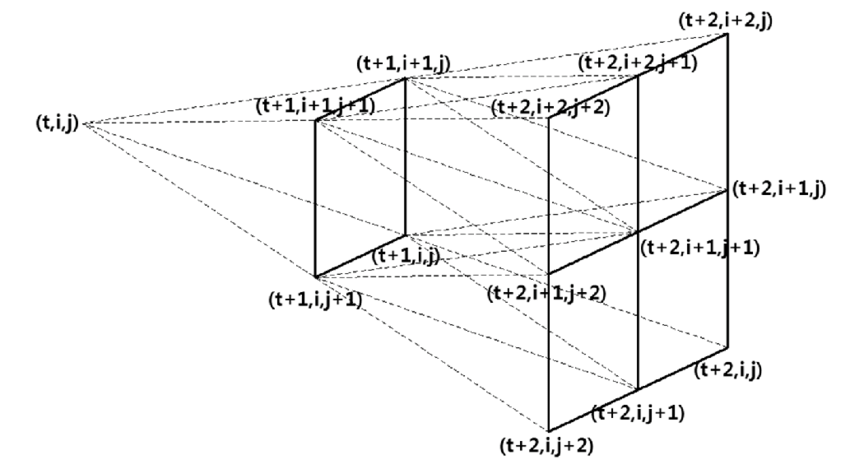
\includegraphics[width=\textwidth]{Figures/Three-dimensional-binomial-lattice.png}
\decoRule
\caption[Three Dimensionel Binomial Lattice]{Evolution of binomial model with two underlying risky asset, where t is time, i is number of up movement for $S_1$ and j is number of up movement for $S_2$  \parencite{Kim02}.}
\label{fig:threeDimLattice}
\end{figure}

After the construction of the evolution of the underlyings, we can like in the one dimensionel CRR model recursively working backward in the multidimensional binomial lattice. For the european option the recursive formula is:
$$V_{i_1,\ldots, i_d}(t)=\exp(-r\Delta t) \bigg(p_1 V_{i_1+1,\ldots, i_d +1}(t+1) + \cdots + p_{2^d} V_{i_1,\ldots, i_d}(t+1) \bigg)$$
For the american option we approximate it with the Burmudan option with N-1 decision points, hence we have the possibility of exercising between inception and maturity of the contract at the decision points hence:
$$V_{i_1,\ldots, i_d}(t)=\max\{\Phi(t,\bm{S}(t)), \exp(-r\Delta t) \bigg(p_1 V_{i_1+1,\ldots, i_d +1}(t+1) + \cdots + p_{2^d} V_{i_1,\ldots, i_d}(t+1) \bigg)\}$$
With the recursive formulas we can valuate multivaraite contigent claims for a variety of exotics including the american put option with several underlying risky assets. The increasing dimensions also increase the number of one-step transition probabilities, hence the \parencite{NEK} approach (NEK) tries with setting all the probabilities equal to 0.5 and than determine the jump sizes. The NEK approach overcome the issue with negative probabilities for higher dimensions and following \parencite{NEK} the algorithm seems also to have faster convergence. The NEK and BEG approaches are both good for low dimensionel option problems, but both still suffers from the curse of dimensionality. The simulations methods on the otherhand has somewhat an advantage for higher dimesions, but e.g. the LSM regression does not scale well for high dimensional rainbow options. We choose to present the BEG approach, because it is a natural extension of the already presented CRR model, which we already build inituition opon. The key for the BEG approach is that we approximate a multivariate lognormal distribution with a discrete distribution. 

\newpage

\section{Least Square Monte Carlo Method}\label{LSM}
From above the binomial model is not suitable for path-dependent contingent claims like an asian option and high dimensional multivariate contingent claims. Simulation methods overcome somewhat this issue. The first monte carlo methods was to use pure simulation techniques, these methods overcome the issue of path-dependent option, but they still suffered the curse of dimensionality. To solve the dimensionality problem the LSM was born, where the idea is combine simulation with regression. The methods presented in this \\

A pure simulation technique have three ingredients a simulation based on the assumption of the underlying asset(s) distribution to price potential future prices. From the simulation of the underlying(s) use the contract function to get the cash flow, then discount back to present value and then average over the simulated paths. The approach is suitable for the asian option, because by simulatation you have the whole path and averaging is straightforward. On the other hand the binomial model is computational fast and accurate for american options, because by discretization the underlying stock the algorithm give an effective way to get intrinsic and expected continuation values. The pure simulation method would not be ideal for american options, because a each decision point for the american option the pure simulation would need to simulate a new set of paths to estimated the expected continuation value. For reference of the pure simulation method is chapter 10 in \parencite{OVERHAUSMARCUS2007EHD}.\\ 

The computer is discrete by nature, so we approximate the american put option with a bermudan put option. The N time points or exercise points chosen between inception and maturity are equidistant time steps and by chosen N sufficient large the bermuda option approximate the american option. Hence the simulatation methods use the setup in section \ref{DiscreteValueFramework}, because we discretize the decision points. We use again dynamic programming to calculate the price of the american put option. The problem with the pure simulation approach is the computational burden to evaluate the expected continuation value at each exercise data. The Longstaff and Schwartz LSM algorithm overcomes the exponential growing computation burden in pure Monte Carlo simulation by using regression to calculate the expected continuation value.

\subsection{The Algorithm}
Before solving the optimal stopping problem numerically, we set up the mathemeatical framework for solving the problem inspired by \parencite{analysislsm}. The optimal problem in discrete time is:
\begin{equation}\label{Bermudanstop}
\sup_{\tau \in \mathcal{T}(0,\ldots,T)} E^Q[G(S(\tau))]
\end{equation}
where $\mathcal{T}(0,\ldots,T)$ is a class of all $(0,\ldots,T)$-valued stopping times and $\bigg(S(0),S(t_1), \ldots, S(t_N)=S(T)\bigg)$ is the underlying stochastic markov process describing e.g. stock price, volatility, average stock price, etc. The markov chain $(S_{t_n})_{n=0,\ldots,N}$ has state space $(E, \mathcal{E})$. Remember the discrete optimal value process is given by
$$U(t_n)=\esssup_{\tau \in \mathcal{T}(t_n,\ldots,t_N)} E^Q[G(S(\tau))|\mathcal{F}_n]$$
The markov property implies that 
$$E^Q[G(S(\tau_{t_{n+1}}))|\mathcal{F}_{t_n}]=E^Q[G(S(\tau_{t_{n+1}}))|S(t_n)]=f(S(t_n))$$ 
and we assume the initial state to be $S(0)=s$ and deterministic. We solve equation \eqref{Bermudanstop} by the theory presented in section \ref{DiscreteValueFramework}, hence the dynamic programming principle on the optimal policy is
\begin{equation}\label{LSMDynamic}
\begin{split}
\begin{cases}
          \tau_{t_N} = t_N\\
          \tau_{t_n} = t_n \cdot 1_{\{G(S(t_n)) \geq E^Q[G(S(\tau_{t_{n+1}}))|\mathcal{F}_{t_n}])\}} + \tau_{t_{n+1}} \cdot 1_{\{G(S(t_n)) < E^Q[G(S(\tau_{t_{n+1}}))|\mathcal{F}_{t_n}])\}} \quad for \ n={0,\ldots,N-1} \\ 
\end{cases}
\end{split}
\end{equation}
Equation \eqref{LSMDynamic} involves many conditions expectations, hence we need an effective algorithm for evaluating them. The first approaches for solving the optimal stopping problem with pure monte carlo was computational expensive, because with pure simulation methods the paths required for evaluate the conditional expectations increases exponential with decision points (chapter 10 \parencite{OVERHAUSMARCUS2007EHD}). The solution to reduce the computational burden is to use least square regression to calculate the expected continuation value suggested e.g. in \parencite{lsm,Tsitsiklis}. \\

The LSM algorithm approximate the condition expectation with respect to $S(t_{n})$ by orthogonal projection on the state-space genereated by finite number of functions of $S(t_{n})$. Define a sequence $(e_{j}(s))_{j\geq 1}$ of real measurable functions defined on $E$ and satisfying:
\begin{enumerate}\label{AssumptionBasisFck}
\item[•] The sequence $(e_{j}(S(t_n)))_{j\geq 1}$ is total in $L^2(\sigma(S(t_n)))$ for $n=1,\ldots,N-1$.
\item[•] if $\sum_{j=1}^{m} \lambda_j e_{j}(S(t_n))=0 \ a.s.$ then $\lambda_j=0$ for $n=1,\ldots,N-1$, $m\geq 1$ and $j=1,\ldots,m$
\end{enumerate}
By defining the vector space generated by $(e_{j}(s))_{j=1, \ldots, m}$ we denote the orthogonal projection from $L^2(\Omega)$ onto the vector space by $P^m_{t_n}$.
We approximate the expected continuation value by the projection
\begin{equation}\label{LSMDynamic2}
\begin{split}
\begin{cases}
          \tau_{t_N}^{[m]} = t_N\\
          \tau_{t_n}^{[m]} = t_n \cdot 1_{\{G(S(t_n)) \geq P^m_{t_n}(G(S(\tau_{t_{n+1}})))\}} + \tau_{t_{n+1}} \cdot 1_{\{G(S(t_n)) < P^m_{t_n}(G(S(\tau_{t_{n+1}}))) \}} \quad for \ n={0,\ldots,N-1} 
\end{cases}
\end{split}
\end{equation}
Where
$$P^m_{t_n}(G(S(\tau^{[m]}_{t_{n+1}})))=\alpha^{m}(t_{n+1}) \cdot e^m(S(t_{n})) \quad for \ n=1,\ldots,N-1$$
and the $\cdot$ on the right hand side is the usual inner product in $\mathbb{R}^m$ and $e^m=(e_1,\ldots, e_m)$.
By solving the above dynamic programming equation the time 0 approximate price of the Bermudan option is:
$$U^m(0)=\max \{ G(S(0)), E^Q[G(S(\tau^{[m]}_{t_1}))]\}$$
Where $G(S(0))$ is deterministic by assumption, but $E^Q[G(S(\tau^{[m]}_{t_1}))]$ needs to be evaluated numerically, where in the LSM algorithm the methods for evaluation the projection is monte carlo simulation.\\

From the assumption about the distribution of the underlying state space we simulate K independent paths $S^{(1)}(t_n), S^{(2)}(t_n), \ldots, S^{(k)}(t_n), \ldots, S^{(K)}(t_n)$ of the Markov chain $S(t_n)$ with gain process $G(S^{(k)}(t_n))$ for $k=1, \ldots, K$ and $n=0,\ldots,N$. The least square estimator $\alpha^{(m,K)}(t_n)\in \mathbb{R}^m$ for the simulated paths of the stochastic process $S$.
\begin{equation}
\alpha^{(m,K)}(t_n)= \argmin_{a\in \mathbb{R}^m} \dfrac{1}{K}\sum_{k=1}^{K} \bigg(G(S^{(k)}(\tau^{k,m,K}_{t_{n+1}}))  -a \cdot e^m(S^{(k)}(t_{n})) \bigg)^2 \quad for \ n=1, \ldots, N-1
\end{equation}
Where the recursively estimated stopping time is defined by:
\begin{equation}\label{LSMDynamic3}
\begin{split}
\begin{cases}
          \hat{\tau}_{t_N}^{k,m,K} = t_N\\
          \hat{\tau}_{t_n}^{k,m,K} = t_n \cdot 1_{\{G(S^{(k)}(t_n)) \geq \alpha^{m,K}(t_{n}) \cdot e^m(S^{(k)}(t_{n})) \}} + \hat{\tau}_{t_{n+1}}^{k,m,K} \cdot 1_{\{G(S^{(k)}(t_n)) < \alpha^{m,K}(t_{n}) \cdot e^m(S^{k}(t_{n})) \}} \quad for \ n={0,\ldots,N-1} \\ 
\end{cases}
\end{split}
\end{equation}
An example of polynomial linear on each decision points is illustrated in figure \ref{fig:LSM1}, where the blue line is the estimated expected continuation value. From following the optimal stopping stragegy by dynamic programming we derive the approximation for $U^{m}(0)$ from the simulated paths. The time 0 approximate price of the Bermudan option is
\begin{equation}
U^{m,K}(0) = \max \{ G(S(0)), \frac{1}{K} \sum_{k=1}^{K} G(S^{(k)}(\hat{\tau}^{k,m,K}_{t_1}))]\}
\end{equation}

\begin{figure}[th]
\centering
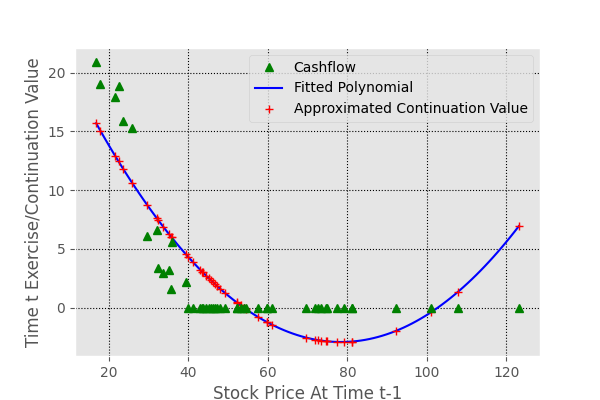
\includegraphics{Figures/LSMFit1.png}
\decoRule
\caption[Polynomial Regression Of Continuation Value]{By zooming in on a specific point of time in backward induction approach, we see how the algorithm regress the continuation value}
\label{fig:LSM1}
\end{figure}

\subsection{American Put}
The optimal stopping problem for an american put 
\begin{equation}\label{optimalStopPut}
\begin{split}
P(0) = \sup_{\tau \in \mathcal{T}(0,\ldots,T)} E^Q[ e^{-r \tau} \cdot \max\{K-S(\tau), 0 \}]
\end{split}
\end{equation}
can be solved with the LSM algortihm. The stock values are modelled via black scholes theory (see path for GBM figure \ref{fig:BM}), hence the simulated evolution for the stock under the risk neutral valuation is given by:
\begin{equation*}
\begin{split}
S_i(t)=S_i(0) \cdot \exp \bigg( \sum_{j=1}^{d}(\sigma_{i,j} W_j(t) -\frac{1}{2} \sigma_{i,j}^2 t) + rt \bigg) \quad  for \ i=1,\ldots,d
\end{split}
\end{equation*}
The stock paths are simulated from inception up to maturty with N-1 decision dates. The focus in this section is on a univariate contingent claim and for convenience we assume the risk free interest rate and volatility is constant. Like in the binomial model, we work backward from maturity to inception at each exercise dates to decide the optimal stopping time. \\

The dynamic programming principle on optimal policy gives the first optimal stopping time. In our setting we regress the expected payoff by continuation of the contract and compare it to the intrinsic value. The dependent variable in the regression is the expected value of continuation and the independent variables is a set of orthogonal basis functions in $L^2(\sigma(S(t_n)))$ of the simulated paths. Typical choices for basis functions could be weighted Laguerre -, Hermit -, and Jacob polynomials. The weighted Laguerre polynomial is given by
\begin{align*}
e_0(S) &= \exp(-S/2) \\
e_1(S) &= \exp(-S/2) (1-S) \\
e_2(S) &= \exp(-S/2) (1-2S+S^2/2) \\
\vdots \\
e_j(S) &= \exp(-S/2) \dfrac{e^S}{j!} \frac{d^j}{dS^j}(S^j e^{-S}) 
\end{align*} 
This kind of regression is a nonlinear expansion of the linear model. We define regressed conditional expectation by:
$$\Psi(S; \alpha)= \sum_{j=0}^p \alpha_j \cdot e_j(S) $$
where $\alpha$ is the coefficients for the regression, e is the basis function, where the argument is the underlying markovian process $S$. By using this iterative method, we arrive at the pathwise optimal stopping policy, where in figure \ref{fig:LSM2} the optimal stopping times are shown. The figure illustrates that the option only can be exercised once, hence the gray lines after the triangles.

\begin{figure}[th]
\centering
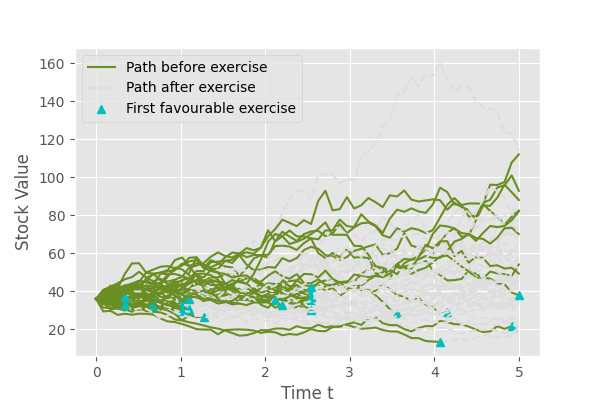
\includegraphics{Figures/LSMFit2.png}
\decoRule
\caption[Optimal Stopping Decision]{The optimal stopping decisions by the Least Square Monte Carlo Method}
\label{fig:LSM2}
\end{figure}


\subsection{Convergence}
In the rigorous approach in \parencite{analysislsm} they show convergence results for the optimal value process or the snell envelope $U$. We will present that $U(0)^{m,K}$ converges almost surely to $U(0)^{m}$ for K goes to infinity, i.e. the approximate value process by simulation and regression on a finite set of functions converge to the approximated value process with truncated orthogonal basis by letting the sample size go to infinity. Furthermore it can be shown that $U(0)^{m}$ converge to $U(0)$ for m goes to infinity. The second result is that the regressed value function converge to the expected continuation value by letting the number of basis function goes to infity. The latter result is shown using the expected continuation values.
\begin{theorem}\label{LSMConvergence1}
Assume the sequence $(e_{j}(S(t_n)))_{j\geq 1}$ is total in $L^2(\sigma(S(t_n)))$ for $n=1,\ldots,N-1$. Then for $n=0,\ldots,N$ we have
$$\lim_{m\to +\infty} E^Q[G(S(\tau_{t_n}^{[m]})) |\mathcal{F}_{t_n}]=E^Q[G(S(\tau_{t_n})) |\mathcal{F}_{t_n}]$$
in $L^2$
\begin{proof}
The proof is given by induction, where the orthogonal basis is total in $L^2$ is important, because $||P^m_{t_n}(E^Q[G(S(\tau_{t_{n+1}}))|\mathcal{F}_{t_n}])- E^Q[G(S(\tau_{t_{n+1}}))|\mathcal{F}_{t_n}]||_2 \to 0 \quad for \ m \to \infty$.
(more details on p. 6-7 \parencite{analysislsm})
\end{proof}
\end{theorem}

The former result is also shown in \parencite{analysislsm}.
\begin{theorem}\label{LSMConvergence2}
Assume the sequence $(e_{j}(S(t_n)))_{j\geq 1}$ is total in $L^2(\sigma(S(t_n)))$ for $n=1,\ldots,N-1$ and if $\sum_{j=1}^{m} \lambda_j e_{j}(S(t_n))=0 \ a.s.$ then $\lambda_j=0$ for $n=1,\ldots,N-1$, $m\geq 1$ and $j=1,\ldots,m$. Futhermore assume that $Q(\alpha_{t_n} \cdot e(S(t_n))=G(S(t_n)))=0$.\\
Then $U^{m,K}(0)$ converges almost surely to $U^{m}(0)$ as K goes to infinity.\\
The proof is out of scope for this thesis, see the article \parencite{analysislsm} for a proof in details. 
\end{theorem}

The two convergence results shows the convergence for the LSM algorithm, hence the LSM will approximate the optimal value process well for sufficient large sample sets and enough basis functions.


\subsection{Upper Bound}
By the results from \parencite{AndersenLeif2004} they provide a algorithm for computing a lower and upper bound for the american option price, where the lower bound is generated by approximating the continuation value. They show with martingale methods that the interval becomes smaller when the lower bound approaches the true value. The true value will always by higher than the approxmixation, because the true value is when you exercise optimal at each decision point. Hence to compare approximation method on the continuation value a higher lower bound indicate a better approximation to the true value.

Given the optimal exercise boundary is only an estimate, both the methods underestimate the "true value" of the option.

A simple comparison would be whichever method produced higher price for the option is better.

For this comparison to make sense, you could

    re-use underlying stock simulation across both the methods.
    make sure variance of price produced is reasonably low for both.

The "better" value of the two is still a lower bound and doesn't really throw information on how big the error is.

You could implement dual method to produce upper bound and thus a range for the true option price.
The regression performed in LSM is only for in money path for improving the algorithm, wher



The LSM approach gives a lower bound for the true price of the option given optimal stopping choice:
\theoremstyle{proposition}
\begin{proposition}{}\label{Lower-Bound-LSM}
\textbf{Lower Bound To True Value:} For any finite choice of M, K, and vector $\theta\in \mathbb{R}^{M \times (K-1)}$ representing the coefficients for the M basis functions at rach of the K-1 early exercise dates, let $LSM(\omega;M,K)$ denote the discounted cash flow resulting from the following the LSM rule of exercising when the immediate exercise value is positive and greater tahn or equal to $\hat{F}_{M}(\omega_{l};t_{k})$ as defined by $\theta$. Then the following inequality holds almost surely,
$$V(X)\geq \lim_{N\to \infty} \dfrac{1}{N}\sum_{i=1}^{N} LSM(\omega_i;M,K)$$
(p. 124 \parencite{lsm})
\end{proposition}


\subsection{LSM Extension To Multivariate Contingent Claims}
For pricing of bivariate and multivariate contingent claims, we have to account for correlation between assets. The correlation matrix $\Sigma$ is given by
\begin{equation}
\Sigma = \begin{pmatrix}
\rho_{1,1} & \rho_{1,2} & \cdots & \rho_{1,d} \\
\rho_{2,1} & \rho_{2,2} & \cdots & \rho_{2,d} \\
\vdots & \vdots & \ddots & \vdots \\
\rho_{d,1} & \rho_{d,2} & \cdots & \rho_{d,d} \\
\end{pmatrix} = \Sigma = \begin{pmatrix}
1 & \rho_{1,2} & \cdots & \rho_{1,d} \\
\rho_{2,1} & 1 & \cdots & \rho_{2,d} \\
\vdots & \vdots & \ddots & \vdots \\
\rho_{d,1} & \rho_{d,2} & \cdots & 1 \\
\end{pmatrix}
\end{equation}
The correlation between assets are given by $(\rho_{i,j})_{i\neq j}$ and each asset has correlation 1 with itself. We assume that $(\rho)_{i \neq j} \in (-\frac{1}{d-1},1]$, because then the correlation matrix is a real, symmetric and positiv definit, hence Cholesky factorization can be utilized $\Sigma=LL^T$ where $L$ is a lower triangular matrix. From the decomposition it is easy to simulate correlated assets in d-dimensional Black-Scholes model:
\begin{equation}
dS_{i}(t)=S_{i}(t) r dt + S_{i}(t) \sigma_i L_{i,\cdot} d\bm{W}(t) \quad i \in \{1,2,\ldots, d\}
\end{equation}
Where $\bm{W}$ has values in $\mathbb{R}^d$ and $\sigma=(\sigma_1, \sigma_2, \ldots, \sigma_d)$ is vector of volatilities.\\

By simulating the paths according to the black scholes dynamic, it is straightforward to apply the LSM, because it follows the same algortihm just with a different contract function.'

\newpage

%----------------------------------------------------------------------------------------
%	SECTION 4
%----------------------------------------------------------------------------------------

\section{Closed Form Solutions For European Exotic Options}\label{ExoticEuro}
Most exotic options require numerical methods, but in some special cases there exist a closed form solution. We will look at some of them in this section, where the purpose is to provide benchmarks for the numerical methods. Furthermore we explore the boundaries of closed form solutions and show applications of martingale theory. Thorughout the financial model and assumptions given in section \ref{MultiDimModel} will be assumed. We derive closed form solutions to european call and put options depending on several variables, for simplicity we will focus on pricing options with 2 or 3 underlying stocks. We apply the intuition given in \parencite{Johnson87} and the results given in \parencite{Ouwehand2006}. The exotic contingent claims we will consider are the geometric mean -, maximum - and minimum call option.

\subsection{Geometric Basket Call Option}\label{GeoBasket}
For a geometric basket call option the contract function is given by:
\begin{align*}
\Phi(S(T))=\max\{ (\prod_{i=1}^{n} S_i(T))^{\frac{1}{n}}-K,0 \}
\end{align*}
The key to  derive a closed form solution is the known result that the sum of normal random variables are multivariate normal distributed.
This implies that the product of lognormal random variables are multivariate log-normal distributed. Since: 
\begin{equation*}
\begin{split}
\exp(x+y)&=\exp(x)\cdot \exp(y) \\
& \text{and}\\
 X \sim \mathcal{N}(\mu,\sigma^2) & \Rightarrow Y = \exp(X)\sim LN(\mu, \sigma^2)
\end{split}
\end{equation*}

Remember the assumption in section \ref{MultiDimModel} that the stocks price process follows a GBM, hence:
\begin{equation}\label{prodGBM}
\begin{split}
(\prod_{i=1}^{d} S_i(T))^{\frac{1}{d}} = (\prod_{i=1}^{d} S_i(0))^{\frac{1}{d}} \exp\bigg((r-\frac{1}{2d}\sum_{i=1}^{d}\sigma_i^2)T + \frac{1}{d} \sum_{i=1}^{d} \sigma_i W_i(T) \bigg)
\end{split}
\end{equation}
By defining
\begin{align}
\tilde{\sigma} = \frac{1}{d} \sqrt{\sum_{i=1}^{d} \sigma_i^2 + 2 \sum_{i\neq j} \rho_{i,j} \sigma_i \sigma_j}\\
F=(\prod_{i=1}^{d} S_i(0))^{\frac{1}{d}} \exp\bigg((r-\frac{1}{2d}\sum_{i=1}^{d}\sigma_i^2)T + \frac{1}{2} \tilde{\sigma}^2 \cdot T \bigg)\\
\epsilon = \frac{\frac{1}{d} \sum_{i=1}^{d} \sigma_i W_i(T)}{\tilde{\sigma} \sqrt{T}} \sim \mathcal{N}(0,1)
\end{align}
Rewrite equation \eqref{prodGBM} by above definitions
$$(\prod_{i=1}^{d} S_i(T))^{\frac{1}{d}} = F \cdot \exp\bigg( -\frac{1}{2} \tilde{\sigma}^2 \cdot T + \tilde{\sigma} \sqrt{T} \epsilon \bigg)$$
This expression is one dimensional and is the stardard GBM solution with zero drift and spot F. This has a known solution with Black-Scholes theory (section \ref{classicBS}) and the geometric mean call option has price
\begin{equation*}
\Pi(t,\mathcal{X})=\exp(-r \cdot (T-t))\bigg(F N(d_1) - K N(d_2) \bigg)
\end{equation*}
where $d_1=\frac{\ln(\frac{F}{K}) + \frac{1}{2} \tilde{\sigma}^2 T}{\tilde{\sigma} \cdot \sqrt{T}}$ and $d_2=d_1-\tilde{\sigma} \sqrt{T}$\\

The fact that the sums of normals is multivariate normal distributed makes the geometric mean option easy to price in the Black-Scholes model, because the high dimensional problems can be treated as 1-dimensional problem like above with the european geometric mean call option.

\subsection{Options On The Maximum Or The Minimum Of Several Assets}
Here we restrict ourselves to consider the case with three underlying stocks like in \parencite{BEG, Ouwehand2006}, but the formula can be generalized to higher dimensions. The contract functions we consider are:
\begin{enumerate}
\item[•] Best of assets or cash: $\Phi(S(T))=\max\{S_1,S_2,\ldots,S_d,K\}$
\item[•] Call on max: $\Phi(S(T))=\max\{\max(S_1,S_2,\ldots,S_d)-K,0\}$
\end{enumerate}
Assume WLOG $d$=4 to avoid cumbersome calculations and notation. The section will heavily use the martingale framework developed in section \ref{MultiDimModel} and stochastic calculus (Appendix \ref{AppendixB}) to value these exotic options. The key is to choose the numeraire to a risky assets instead of the bank account. By results from section \ref{MultiDimModel} the processes are still Q-martingales given the numeraire is strictly postive. Under the asssumption of a arbitrage free and complete market it follows from risk neutral valuation formula(RNVF).
$$S_0(t)E^{Q_0}_t[\frac{X}{S_0(T)}]=S_1(t)E^{Q_1}_t[\frac{X}{S_1(T)}]$$
This show that changing the numaraire does not change the price of the above derivative.

\subsubsection{Best Of Assets Or Cash}
The best of assets derivative will provide the foundation for pricing call on maximum or minimum of several assets. The best of assets derivative pay out the price of the most valuable asset. The idea is then to set up 4 cases, where in each case a new asset gives a payout if it is the most valuable out of the four cases. This can be written with a indicator, where the payoff for the $i$'th asset is:
\begin{equation}\label{ithPayoff}
S_i(T) \cdot 1_{\{S_i(T)>S_j(T): i\neq j\}} \quad i=\{1,2,3,4\}
\end{equation}

From equation \eqref{ithPayoff} we see that the i'th assets is only different from zero, when it is the most valuable asset. The best of asset derivative is then a sum of 4 terms (remember d=4), where each term is equation \eqref{ithPayoff} for a specific asset $i$. Hence the best of asset derivative can be consider as a sum of 4 derivatives, where we apply RNVF (proposition \ref{RNVF}) for each of them.\\

Let us first consider i=1 and we set $S_1$ to be the numeraire asset with martingale measure $\mathbb{Q}_1$. Then by RNVF:
\begin{equation}\label{ithDerivative}
\begin{split}
\Pi_1(t, \mathcal{X})&=S_1(t)E_t^{Q_1}[1_{\{S_1(T)>S_2(T), S_1(T)>S_3(T), S_1(T)>S_4(T)\}}]\\
&=S_1(t) Q_1[\ln(\frac{S_2(T)}{S_1(T)})<0, \ln(\frac{S_3(T)}{S_1(T)})<0, \ln(\frac{S_4(T)}{S_1(T)})<0]
\end{split}
\end{equation}
From above discussion the derivative price can be found by cycling through the 4 derivatives and add together the prices of the four derivatives. The fair price for best of assets option $\Pi_{max}(t,\mathcal{X})$ is then given as the sum of the 4 derivatives. The above derivative equation \eqref{ithDerivative} needs to be evaluate, therefore we seek to evaluate the probaility under the $Q$-martingale measure. By Ito's lemma (see \ref{Ito}) the discounted process with stock j is
\begin{align}
d(\dfrac{S_i(t)}{S_j(t)})=\frac{S_i(T)}{S_j(T)} \cdot (a_i-a_j)dW^{Q_j}(t) 
\end{align}
where $dW^{Q_j}(t)$ is standard d-dimensional $Q_j$-Wiener process and $a_i$ is the i'th row of the covariance matrix. From the known solution of the GBM we have the distribution.
\begin{align*}
\ln(\frac{S_i(T)}{S_j(T)})\sim \mathcal{N}\bigg(\ln(\frac{S_i(t)}{S_j(t)}) - \frac{1}{2}\sigma_{i/j}^2 \cdot (T-t), \sigma_{i/j}^2 (T-t)\bigg)
\end{align*}
where $\sigma_{i/j}=(a_i-a_j)$ and $\sigma_{i/j}^2=\sigma_i^2+\sigma_j^2-2\rho_{ij}\sigma_i \sigma_j$.\\

Besides using the definition for $d_1$ and $d_2$ in proposition \ref{BS-price-EuroCall} we define:
\begin{align}
d^{i/j}_1 =\frac{1}{\sigma_{i/j}\cdot \sqrt{T-t}} \cdot \bigg( \ln(\frac{S_i(t)}{S_j(t)}) + \frac{1}{2} \sigma_{i/j}^2 \cdot (T-t) \bigg)\\
d^{i/j}_2=d^{i/j}_1-\sigma_{i/j} \sqrt{T-t}
\end{align}
The correlation between $\frac{S_i(T)}{S_k(T)}$ and $\frac{S_j(T)}{S_k(T)}$ is:
\begin{align}
\rho_{ij,k}&:= \dfrac{(a_i-a_k)\cdot(a_j-a_k)}{||a_i-a_k|| \cdot ||a_j-a_k||}\\
&=\frac{\rho_{ij}\sigma_i \sigma_j - \rho_{ik}\sigma_i \sigma_k - \rho_{kj}\sigma_k \sigma_j + \sigma_k^2}{\sqrt{(\sigma_i^2 + \sigma_k^2 - 2\rho_{ik}\sigma_i \sigma_k)\cdot(\sigma_j^2 + \sigma_k^2 - 2\rho_{jk}\sigma_j \sigma_k)}}
\end{align}
Hence:
$$Q_1[\ln(\frac{S_2(T)}{S_1(T)})<0, \ln(\frac{S_3(T)}{S_1(T)})<0, \ln(\frac{S_4(T)}{S_1(T)})<0]=N_3(-d_2^{2/1},-d_2^{3/1},-d_2^{4/1}, \rho_{23,1}, \rho_{24,1}, \rho_{34,1})$$
Cycling through each derivative, we get:
\begin{equation}\label{BestAsset}
\begin{split}
\Pi_{max}(t,\mathcal{X})&=S_1(t) N_3(-d_2^{2/1},-d_2^{3/1},-d_2^{4/1}, \rho_{23,1}, \rho_{24,1}, \rho_{34,1}) \\
&+S_2(t) N_3(-d_2^{1/2},-d_2^{3/2},-d_2^{4/2}, \rho_{13,2}, \rho_{14,2}, \rho_{34,2})\\
&+S_3(t) N_3(-d_2^{1/3},-d_2^{2/3},-d_2^{4/3}, \rho_{12,3}, \rho_{14,3}, \rho_{24,3}) \\
&+S_4(t) N_3(-d_2^{1/4},-d_2^{2/4},-d_2^{3/4}, \rho_{12,4}, \rho_{13,4}, \rho_{23,4})
\end{split}
\end{equation}
We can extend the above result to best of assets and cash by letting $S_4(t)=K\exp(-r(T-t))$, where K do not have any volatilty and also independent of the other assets, hence \eqref{BestAsset} becomes:
\begin{equation}\label{BestAssetOrCash}
\begin{split}
\Pi_{max}(t,\mathcal{X})&=S_1(t) N_3(-d_2^{2/1},-d_2^{3/1},d_1^{1}, \rho_{23,1}, \rho_{24,1}, \rho_{34,1}) \\
&+S_2(t) N_3(-d_2^{1/2},-d_2^{3/2},d_1^{2}, \rho_{13,2}, \rho_{14,2}, \rho_{34,2})\\
&+S_3(t) N_3(-d_2^{1/3},-d_2^{2/3},d_1^{3}, \rho_{12,3}, \rho_{14,3}, \rho_{24,3}) \\
&+K\cdot \exp(-r(T-t)) N_3(-d_2^1,-d_2^2,-d_2^3, \rho_{12}, \rho_{13}, \rho_{23})
\end{split}
\end{equation}

\subsubsection{Call On Max And Call On Min}
From the price of the best of asset or cash option equation \eqref{BestAssetOrCash} the call max option price can be derived. Note that
$$\max\{\max\{ S_1,S_2,S_3 \} - K, 0\}=\max\{\max\{ S_1,S_2,S_3 \}, K\} - K = \max\{ S_1,S_2,S_3,K \} - K$$
The call on max option is then a best of asset or cash option subtracted the strike. Realizing that fact it is easy to price the call on max:
\begin{equation}\label{callMax}
\begin{split}
\Pi_{cmax}(t,\mathcal{X})&=S_1(t) N_3(-d_2^{2/1},-d_2^{3/1},d_1^{1}, \rho_{23,1}, \rho_{24,1}, \rho_{34,1}) \\
&+S_2(t) N_3(-d_2^{1/2},-d_2^{3/2},d_1^{2}, \rho_{13,2}, \rho_{14,2}, \rho_{34,2})\\
&+S_3(t) N_3(-d_2^{1/3},-d_2^{2/3},d_1^{3}, \rho_{12,3}, \rho_{14,3}, \rho_{24,3}) \\
&-K \exp(-r(T-t)) \cdot\bigg(1 - N_3(-d_2^1,-d_2^2,-d_2^3, \rho_{12}, \rho_{13}, \rho_{23})\bigg)
\end{split}
\end{equation}

To derive put max we can utilize a put-call-parity (see page 6 \parencite{Ouwehand2006}), but it takes a different form than the one presented in \ref{Chapter2} (see \ref{put-call-parity}). The relationship for the exotic call options:
$$V_c(K)+K\exp(-r\cdot (T-t)) = V_p(K)+V_c(0)$$
Where $V_c(K)$ is the value of the exotic call option and $V_c(0)$ is the best of assets call option.\\

The exotic european options serve as benchmark for the multivariate lattice approach, because if the lattice appproach is close to the european benchmark then it is reasonable to expect a close estimat to the american option. The above section is also a presentation of the martingale approach versatility. 




% Chapter Template

\chapter{Deep Learning} % Main chapter title

\label{Chapter4} % Change X to a consecutive number; for referencing this chapter elsewhere, use \ref{ChapterX}

The chapter is inspired by \parencite{Goodfellow-et-al-2016,Mackay18} where the interested reader can find more information about deep learning. Deep learning experiences a renaissance, because of the technology improvements in hardware and software. The collection of data has also significantly improved the field. Deep learning is a specialized field in machine learning, where you focus on a special architecture of models. Like in machine learning the basic components of a deep learning algorithm are a data set, cost function, optimization algorithm, and a model. E.g. in the LSM method we assumed the linear model, data set was the simulated paths, the cost function was the mean squared error and the optimization algorithm was a closed form solution of the normal equations. Deep learning is about studying neural networks which allows for greater flexibility than standard methods like linear regression. \\

A neural network consists of multiple layers, where the depth tells you how many layers the network has (figure \ref{fig:multilayer-perceptron}), hence, the name "Deep learning". All the algorithms applied will be within supervised learning, where we try to fit the best relationship between the features and the response variable. Furthermore, all our algorithms will be based on the multilayer perceptrons (MLPs) model for regression, therefore, most of the chapter presents the theory for supervised MLPs regression. The advantage of a multilayer model is that for each layer the updated set of covariates can be more finely tuned to better explain the data making the model extremely flexible. The MLPs is also called feedforward neural networks, because the information only travels forward in the neural network, through the input node(s) then through the hidden layer(s) and finally through the output node(s). First, we present the basics for machine learning and then specialize the theory to deep learning.

%----------------------------------------------------------------------------------------
%	SECTION 1
%----------------------------------------------------------------------------------------

\section{Machine Learning Basics}
The task for machine learning is to learn from data with respect to some performance measure. "A computer program is said to learn from experience E with respect to some class of tasks T and performance measure P, if its performance at tasks in T, as measured by P, improves with experience E" (\parencite{Goodfellow-et-al-2016} p. 97). Classical tasks T could be classification or regression, where the two methods differ on the output type. The former has discrete outputs, where regression has continuous output. We seek to find a price, which is naturally represented as a continuous value. Hence, our task will be to regress the price or expected continuation value. Measuring performance depends on the task, but for regression a typical performance measure is mean squared error (MSE):
$$\frac{1}{K}\sum_{k=1}^{K} (y_k-\hat{y}_k)^2$$
There are other methods for measuring performance, e.g. mean absolute error (MAE). Another measure to quantify the fit is coefficient of determination:
$$R^2=1-\frac{\frac{1}{K}\sum_{k=1}^{K} (y_k-\hat{y}_k)^2}{\frac{1}{K}\sum_{k=1}^{K} (y_k-\bar{y})^2} \quad \text{where $\bar{y}$ is the sample mean}$$
Coefficient of determination explains how well the model explains the data compared to the empirical mean. Some care should be taken when comparing models with different capacities, because the coefficient of determination will tend to prefer the larger models. The experience comes from data, where the data can be given with or without target values $\bm{y}$. In machine learning the task is quite different depending on if targets are given or not. Hence, the algorithms are split into two categories; supervised and unsupervised learning. The terminology \textsl{"supervised"} comes from a teacher that gives you the target values $\bm{y}$ that the algorithms tries to predict from $\matr{X}$.\\

Machine learning is not about making overly complex models to fit your data perfectly, because then the model will most likely have poor performance on unseen data. This phenomenon is known as overfitting, but the models can also be too simple, known as underfitting. If machine learning only cared about performance on the given data for training, then machine learning would be essentially optimization. The key difference is that machine learning wishes to obtain statistical generalization to unseen data. The practical way to evaluate the model is to measure generalization error on a test set. In machine learning the data is split into test data and training data, where the test set can only be used for evaluation after training. \\

The training data is used for training the model, where the training error shows how the fitted parameters fit to the training data. An unacceptable high training error could indicate that the regression method could be too simple and underfitting is the issue. For training it can sometimes also be useful to have a validation data set to see how your model generalizes, because the test set cannot be used to make model choices. It is common to split the training set into a validation and training set. The validation set is allowed to be used in training and it tries to mimic the generalization error. A common technique for measuring validation errors is \textsl{"cross-validation"}, where the data set is split into training and validation sets depending on the cross-validation scheme. The aim for the validation data is to approximate the model performance on unseen data, which is essentially what we want to have within an acceptable range.\\

After training the model we can evaluate the performance on a test set not seen in training. An unacceptable high test error when evaluating the model and very low training error could be an example of overfitting the model. Hence, when training the model, we want the best of both worlds; an acceptable training error, as well as making the gap between training and test error acceptable as well. In machine learning the overfitting and underfitting concepts are expressed by the relation of a bias-variance trade-off, where the trade-off is between training error and generalization error. In case of overfitting, the model has been extensively trained to get a low biases, but the trade-off is that the model does not generalize well represented by a high variance.\\

A technique known as regularization is one approach to avoid overfitting. The regularization term is added to the cost function $J(\theta)$, which is essentially the function to minimize in order to train the model. There are many different regularization methods, where in section \ref{multilayerPerceptron} we will present some useful methods for deep learning models. Besides the parameters estimated within the model, there are many parameters called hyperparameters exogenous given by the model designer.\\

Hyperparameters are the parameters not estimated within the model. Some common examples of hyperparameters in machine learning and deep learning are the learning rate, batch size, weight decay, model capacity, etc. The choice of the hyperparameters is often more important than the optimization algorithm chosen to estimate the parameters within the model. Hence, the need for suitable choices for hyperparameters is required for having an high quality machine learning model. The calibration of the model to a specific task is called hyperparameter tuning, where it can be done manually or automatically. The manual choice requires expert knowledge to set the hyperparameter optimal for the given task, where the automatic procedures are often computationally expensive. Examples of hyperparameters tuning rutines are random search, grid search, and Bayesian optimization.\\

The parameters within the model are found by minimizing the cost function $J(\theta)$. In some cases there exists either a closed form solution or the cost function is convex, making the optimization problem easier to handle. The complexity of MLPs makes the cost function non convex and iterative optimization procedures are needed. The basic iterative procedure is the gradient descent where the concept is to repeatedly making small moves in parameters toward better configuration. The most popular gradient methods in deep learning are Adam, RMSProp, AdaGrad, and stochastic gradient descent (SGD). The methods will be discussed in more details in section \ref{trainNetwork}. To sum up, a machine learning model needs a data set, a model, a cost function, and an optimization algorithm. Understanding of basic machine learning will be the foundation for deep learning.


%----------------------------------------------------------------------------------------
%	SECTION 2
%----------------------------------------------------------------------------------------

\section{Multilayer Perceptrons}\label{multilayerPerceptron}
The goal of the multilayer perceptrons (MLPs) is to approximate a function $f^*(x)$, where the MLPs defines a mapping $x\in \mathbb{R}^R \mapsto f(x;\theta)$ to approximate $f^*(x)$. The task is to find the best $\theta$ such that the approximation $f(x;\theta)$ is close to the targets measured by a defined cost function $J(\theta)$. With the minimized cost function we seek to archive statistical generalization, i.e. good results for test data not used for training. \\

The first step for MLPs is building the network, where we begin with zooming in on a single neuron, which is one node of the directed acyclic graph (figure \ref{fig:multilayer-perceptron}). Note that the MLPs is also called a feedforward network, because all the connections between the neurons are directed so that the network forms a directed acyclic graph.

%-----------------------------------
%	SUBSECTION 1
%-----------------------------------
\subsection{A Single Neuron}\label{singleNeuron}
The single neuron has $R$ features $x_r$ as inputs and one output $\hat{y}$ (figure \ref{fig:singleNeuron}). 

\tikzset{%
  every neuron/.style={circle,draw,minimum size=1cm},
  neuron missing/.style={draw=none,scale=4,text height=0.333cm,execute at begin node=\color{black}$\vdots$},
}
\begin{center}
    \begin{figure}[h]
        \begin{tikzpicture}[
        		init/.style={
 				draw,
  				circle,
  				inner sep=2pt,
  				font=\Huge,
  				join = by -latex
			},
			squa/.style={
  				draw,
  				inner sep=2pt,
  				font=\Large,
  				join = by -latex
			},
			start chain=2,node distance=13mm
			]
			\node[on chain=2] 
			  (x2) {$x_2$};
			\node[on chain=2,join=by o-latex] 
			  {$w_2$};
			\node[on chain=2,init] (sigma) 
			  {$\displaystyle\Sigma$};
			\node[on chain=2,squa,label=above:{\parbox{2cm}{\centering Activate \\ function}}]   
			  {$g$};
			\node[on chain=2,label=above:Output,join=by -latex] 
			  {$y$};
			\begin{scope}[start chain=1]
			\node[on chain=1] at (0,1.5cm) 
 				(x1) {$x_1$};
			\node[on chain=1,join=by o-latex] 
				  (w1) {$w_1$};
			\end{scope}
			\begin{scope}[start chain=3]
				\node[on chain=3] at (0,-1.5cm) 
				  (x3) {$x_3$};
				\node[on chain=3,label=below:Weights,join=by o-latex] 
			 	 (w3) {$w_3$};
			\end{scope}
			\node[label=above:\parbox{2cm}{\centering Bias \\ $w_0$}] at (sigma|-w1) (b) {};

			\draw[-latex] (w1) -- (sigma);
			\draw[-latex] (w3) -- (sigma);
			\draw[o-latex] (b) -- (sigma);

			\draw[decorate,decoration={brace,mirror}] (x1.north west) -- node[left=10pt] {Inputs} 				(x3.south west);
        \end{tikzpicture}
        \caption{A Single Neuron}
        \label{fig:singleNeuron}
    \end{figure}
\end{center}



The function from inputs to output for a single neuron is:
\begin{align*}   
\hat{y}=g(w_0 + \bm{x}^T \bm{w}) \quad where \quad \bm{x}=\begin{pmatrix}
x_1 \\
\vdots\\
x_R
\end{pmatrix} \quad and \quad \bm{w}=\begin{pmatrix}
w_1 \\
\vdots \\
w_R
\end{pmatrix}
\end{align*}
The $\bm{w}$ is the weight matrix (this case a vector) and $w_0$ is the bias term. The term inside the function g is the activation of the neuron and it is a affine transformation denoted:
$$a= w_0 + \bm{x}^T \bm{w}$$
The function g is the activation function and it is essential for the flexibility of the MLPs. There exists numerous of activation functions, only the imagination is the limit. We will list the most common and discuss them.


%-----------------------------------
%	SUBSUBSECTION 1
%-----------------------------------
\subsubsection{Activation Functions}
Activation functions are essential for neural network, because they allow for non-linearities and flexibility. Activation functions apply a non-linear transformation and decide whether a neuron should be activated or not. Without activation functions or the activation function being the identity function $g(a)=a$, the whole network would essentially be a linear regression model. Some popular activation functions are:
\begin{enumerate}
\item[•] Sigmoid function: $g(a)=\frac{1}{1+\exp(-a)}$\\

This is the traditional choice, also called the logistic function. Popular in classification, but can suffer from vanishing gradient in deep learning.
\item[•] Hyperbolic tangent function: $g(a)=\frac{e^a-e^{-a}}{e^a+e^{-a}}$\\

A scaled and shifted sigmoid function and likewise, suffers from the vanishing gradient problem. The range is $(-1,1)$ and centered at zero. Often used for hidden layers.
\item[•] ReLU function: $g(a)=\max(0,a)$.\\

Rectified Linear Unit is one of the most popular choices since it does not suffer from the vanishing gradient problem. The MLPs often becomes more sparse because it sets some features to zero. It is claimed that ReLU learns multiple times faster than both the hyberbolic tangent and the sigmoid function.
\item[•] Leaky ReLU function:  \[ g(a)=
    \begin{dcases}
        a & if \ a \geq 0 \\
        \alpha \cdot a & otherwise \\
    \end{dcases}
\]\\
A disadvantage of ReLU is that some neurons may die out if the neurons are mapped to zero. The Leaky ReLU is designed to give such neurons a chance to get back into action, but not too easily, so $\alpha>0$ is chosen small ( typical $\alpha=0.01$ ) 

\item[•] ELU - exponential linear unit:  \[ g(a)=
    \begin{dcases}
        a & if \ a \geq 0 \\
        \alpha(\exp(a)-1) & otherwise \\
    \end{dcases}
\]\\
Like the Leaky ReLU the ELU is designed to avoid the dead ReLU problem and the $\alpha$ is often chosen to be 1. 
\end{enumerate}

With a understanding of a single neuron we continue to the architecture of a MLPs.


%-----------------------------------
%	SUBSECTION 2
%-----------------------------------
\subsection{Architecture of MLPs}\label{architectureMLPs}
A MLPs consists of a input layer, where all $R$ features enter, $L$ hidden layers, and an output layer. Each hidden layer and the output layer consists of multiple neurons, where the width of the layer is the number of neurons in that layer ($m^l$) (figure \ref{fig:multilayer-perceptron}). The network's inputs are called the input layer, the output layer is the output of the neural network. The layers between the input and output layer are hidden layers. This could be an explanation of why the field is called Deep learning, because of a deep structure of layers. In each hidden layer a linear combination of the features from the previous layer is made and an activation function is then applied in order to create the new hidden features in that layer (figure \ref{fig:multilayer-perceptron}). The MLPs is essential a large nested function, where the inputs go through a chain of functions until reaching the output.
\begin{align*}
\bm{f}(\bm{x};\bm{\theta})=\bm{f}_1 \circ \bm{f}_2 \circ \cdots \circ \bm{f}_{L+1}\\
where \ \bm{f}_i : \mathbb{R}^{m^{i-1}} \to \mathbb{R}^{m^{i}} \quad i=1,\ldots, L+1
\end{align*}
Each function in the composition of functions corresponds to a layer of neurons.
\begin{align*}
\bm{f}_i(x)=\bm{g}(\matr{W}^T \bm{x} + \bm{w_0}) \quad x\in \mathbb{R}^{m^{i-1}}, \ \matr{W} \in \mathbb{R}^{\bm{m^{i-1}} \times \bm{m^{i}} }, \ and \ \bm{w}_0 \in \mathbb{R}^{\bm{m}^{i}}
\end{align*}
So the function maps a vector to a vector, the hidden layers will often be denoted $\bm{h}$ where for each single neuron, we map a vector to a scalar by:
$$h_i=g(\bm{x}^T \cdot \matr{W}_{:,i} + (w_0)_{i})$$
A layer is a vector of neurons, hence, the transformation from one layer to the next can be interpreted as multiple vector to scalar transformations, where each neuron acts in parallel. The different view motivates the initial presentation of single neuron network (section \ref{singleNeuron}).

\usetikzlibrary{decorations.pathreplacing}
\usetikzlibrary{fadings}
\begin{figure}[th]
	\centering
	\begin{tikzpicture}[shorten >=1pt]
		\tikzstyle{unit}=[draw,shape=circle,minimum size=1.15cm]
		%\tikzstyle{hidden}=[draw,shape=circle,fill=black!25,minimum size=1.15cm]
		\tikzstyle{hidden}=[draw,shape=circle,minimum size=1.15cm]
 
		\node[unit](x0) at (0,3.5){$x_1$};
		\node[unit](x1) at (0,2){$x_2$};
		\node at (0,1){\vdots};
		\node[unit](xd) at (0,0){$x_R$};
 
		\node[hidden](h10) at (3,4){$x_1^{(1)}$};
		\node[hidden](h11) at (3,2.5){$x_2^{(1)}$};
		\node at (3,1.5){\vdots};
		\node[hidden](h1m) at (3,-0.5){$x_{m^{(1)}}^{(1)}$};
 
		\node(h22) at (5,0){};
		\node(h21) at (5,2){};
		\node(h20) at (5,4){};
		
		\node(d3) at (6,0){$\ldots$};
		\node(d2) at (6,2){$\ldots$};
		\node(d1) at (6,4){$\ldots$};
 
		\node(hL12) at (7,0){};
		\node(hL11) at (7,2){};
		\node(hL10) at (7,4){};
		
		\node[hidden](hL0) at (9,4){$x_1^{(L)}$};
		\node[hidden](hL1) at (9,2.5){$x_2^{(L)}$};
		\node at (9,1.5){\vdots};
		\node[hidden](hLm) at (9,-0.5){$x_{m^{(L)}}^{(L)}$};
 

		\node[unit](y2) at (12,2){$f(x;\theta)$};
 
		\draw[->] (x0) -- (h11);
		\draw[->] (x0) -- (h1m);
		\draw[->] (x0) -- (h10);
 
		\draw[->] (x1) -- (h11);
		\draw[->] (x1) -- (h1m);
		\draw[->] (x1) -- (h10);
 
		\draw[->] (xd) -- (h11);
		\draw[->] (xd) -- (h1m);
 		\draw[->] (xd) -- (h10);
 		
		\draw[->] (hL0) -- (y2);
 
		\draw[->] (hL1) -- (y2);
 
		\draw[->] (hLm) -- (y2);
 
		\draw[->,path fading=east] (h10) -- (h21);
		\draw[->,path fading=east] (h10) -- (h22);
		\draw[->,path fading=east] (h10) -- (h20);
		
		\draw[->,path fading=east] (h11) -- (h21);
		\draw[->,path fading=east] (h11) -- (h22);
		\draw[->,path fading=east] (h11) -- (h20);
		
		\draw[->,path fading=east] (h1m) -- (h21);
		\draw[->,path fading=east] (h1m) -- (h22);
		\draw[->,path fading=east] (h1m) -- (h20);
		
		\draw[->,path fading=west] (hL10) -- (hL0);
		\draw[->,path fading=west] (hL11) -- (hL0);
		\draw[->,path fading=west] (hL12) -- (hL0);
		
		\draw[->,path fading=west] (hL10) -- (hL1);
		\draw[->,path fading=west] (hL11) -- (hL1);
		\draw[->,path fading=west] (hL12) -- (hL1);
		
		\draw[->,path fading=west] (hL10) -- (hLm);
		\draw[->,path fading=west] (hL11) -- (hLm);
		\draw[->,path fading=west] (hL12) -- (hLm);
		
		\draw [decorate,decoration={brace,amplitude=10pt},xshift=-4pt,yshift=0pt] (-0.5,4) -- (0.75,4) node [black,midway,yshift=+0.6cm]{input layer};
		\draw [decorate,decoration={brace,amplitude=10pt},xshift=-4pt,yshift=0pt] (2.5,4.5) -- (3.75,4.5) node [black,midway,yshift=+0.6cm]{$1^{\text{st}}$ hidden layer};
		\draw [decorate,decoration={brace,amplitude=10pt},xshift=-4pt,yshift=0pt] (8.5,4.5) -- (9.75,4.5) node [black,midway,yshift=+0.6cm]{$L^{\text{th}}$ hidden layer};
		\draw [decorate,decoration={brace,amplitude=10pt},xshift=-4pt,yshift=0pt] (11.5,2.75) -- (12.75,2.75) node [black,midway,yshift=0.5cm]{output layer};
	\end{tikzpicture}
	\caption[Multilayer Perceptrons with $(L+1)$-layers]{Multilayer perceptrons with $(L+1)$-layers with $R$ input features and 1 output. The $l^{\text{th}}$ hidden layer contains $m^{(l)}$ hidden neurons}
	\label{fig:multilayer-perceptron}
\end{figure}

So the MLPs is not like the linear model in section \ref{LSM}, where a single transformation from input to output is applied. The unique attribute of neural network is the ability to approximate any kind of function\footnote{Universal Approximate Theorem page 194 \parencite{Goodfellow-et-al-2016}}, because of the flexibility with applying multiple functions to the input layer. The neural network has a lot of different design options, where e.g. hidden layers, layer width, depth, activation functions etc., are hyperparameters. In general, it is recommended to use many hidden covariates (neurons) rather than too few. The danger of overfitting is than avoided by introducing some kind of penalty to avoid that the model becomes overly complex, which we will discuss further in section \ref{regularization}.\\

To measure the performance of the model, we need a function to measure the difference between the approximation $f(\bm{x};\bm{\theta})$ and the target values $f^*(\bm{x})$. The function used to quantify this approximation is the cost function. The cost function is key to improving our model, in machine learning lingo training the model, and the next section will show why.

%-----------------------------------
%	SUBSECTION 3
%-----------------------------------
\subsection{Training the Network}\label{trainNetwork}
Training the network is key for building a high quality model. The performance of the model is measured by the cost function, where the cost function used in this thesis is the the empirical risk function.
\begin{align*}
J(\theta)=E_{(\bm{x},y)\sim \hat{p}_{data}} L(f(\bm{x};\bm{\theta)},y)= \frac{1}{K}\sum_{k=1}^{K} L(f(x_k;\theta),y_k)
\end{align*}
The loss function $L$ in the empirical risk function for training is chosen to be quadratic, hence, for training we measure the error with mean squared error (MSE) as our cost function.\\

From the above, we see that the cost function is a way to measure the approximation of $f^*(x)$ by our model $f(\bm{x};\bm{\theta})$. The training is important, e.g., imagine after random initialization of parameter and construction of the MLPs we reported the output given the inputs of the model. This model would probably results in a high cost function value, because the given weights would produce a function that does not fit training data. The way out of the high cost function is to minimize the cost function over the weightspace. Therefore, training for MLPs is essentially a optimization of a non convex function. Remember the MLPs is a chain of functions (section \ref{architectureMLPs}) where the structure often makes the optimization a non convex problem. Hence, a global minimum is seldomly archived. Other pitfalls for optimization of MLPs are weight symmetry, steep cliffs, saddle points, vanishing gradients, and exploding gradients.\\

The actual optimization algorithms for MLPs are based on gradients, where we make small local moves. The overall goal is to find the $\theta$ to achieve lowest possible test error. Within gradient methods there are batch gradient descend and mini-batch stochastic gradient descend, where the former is training on the whole data set, and the latter is only for a subset of the data set. The mini-batch methods have the advantage that the method can be parallelized for faster training. An epoch is the number of complete data set training cycles to update the weights. For the mini-batching techniques it is important to randomly sample from the whole data set in order to get unbiased gradient estimation. \\

The goal of the optimization algorithms is to find critical points $\nabla J(\theta)=0$, hence, to obtain the critical points the iterative methods move in the opposite direction of sign of derivative $\nabla J(\theta)$. I.e. the gradient tells us how to update the parameters with a step size called the learning rate $\eta$:
$$\theta_{new}=\theta_{old} - \eta \nabla J(\theta_{old}) $$
$J(\theta)$ is the cost function, hence remember we use the MSE:
$$J(\theta)= \frac{1}{K}\sum_{k=1}^{K} L(f(x_k;\theta),y_k)=\frac{1}{K}\sum_{k=1}^{K} (y_k-\hat{y}_k)^2$$
Common methods to estimate the parameters are gradient descent, stochastic gradient descent (SGD) and Adam, where all the optimization algorithms are iterative. Gradient descend uses the whole batch for each update, where Adam and SGD use mini-batches for each update. The Adam algorithm uses a adaptive learning rate, where the two others use constant or descending learning rates. The Adam method has greater progress in more gently sloped directions of weightspace compared to SGD and gradient descent. \\

Apart from choosing a optimization procedure, the initialization of the parameters are important. There are many suggestions to initialize parameters, but there is no general golden rule at the moment, because of a lack of understanding the optimization procedure in neural networks. Often, the practitioners tend to use simple and heuristic methods, where it has been shown that the initialization breaks weight symmetry.\\

The most common way of finding gradients is the backpropagation algorithm, where the basic idea is the chain rule from calculus.
$$\frac{dz}{dx}= \frac{dz}{dy} \frac{dy}{dx}$$
To understand backpropagation it is often useful with a computational graph created by forward propagation, where the backpropagation computes the derivative from output layer to input layer, by going backwards in the computational graph. The training process is a forward-backward algorithm. Different starting values of $\theta$ will result in different parameters. The good news is that these predictors typically do not differ by very much. It is recommended to work with a set of different starting values and then use as a final predictor the average of the individual predictors originating from each starting value.

%-----------------------------------
%	SUBSECTION 4
%-----------------------------------
\subsection{Regularization}\label{regularization}
The number of parameters and the capacity of neural networks often resilt in overfitting, i.e. the model does not generalize well on new data. Regularization is a technique that alters our optimization problem to discourage complex models, hence, avoiding the problem of overfitting. Some common methods for deep learning are parameter norm regularization, early stopping, and dropout.\\

Early stopping is an effective and simple method for regularization. Compared to parameter norm regularization, the early stopping algorithm does not harm the learning dynamics. The early stopping method is also computationally efficient, and therefore, it is a popular regularization method for deep learning. The idea of early stopping is that the iterative training algorithm keeps improving the train error, but training too extensively leads the the gap between training and test error to increase. The idea is then to split your data into validation and train data sets, where you determine the best $\hat{\theta}$ and the corresponding training steps $\hat{i}$ by iterative comparing the cost function on the validation set. The algorithm stops after a predefined number of steps without improving the cost function on the validation set. The number of epochs to wait for the cost function not to improve is called the patient for the early stopping algorithm.\\

Like early stopping the dropout method is computationally inexpensive. The idea is to remove neurons randomly at each training loop, i.e. when updating the gradient, each node is kept with probability $p$, independently of each other. To perform dropout, a binary mask is sampled independently for each iterations, where the probability $p$ for 1 is another hyperparameter. The goal is to minimize $E_{\bm{\mu}} J(\bm{\theta}, \bm{\mu})$ where $\bm{\mu}$ is the mask. The results of the procedure are more robust features and a regularizing effect on most models.\\

There are many design options for deep learning, where the choices should be specific for the given task. There is a no free-lunch theorem for machine learning, which says no model is superior for all tasks (page 114 \parencite{Goodfellow-et-al-2016}). The designs for specific tasks are important where training error and test error can be improved by designing the model for the given task. Another aspect is the computational resources, i.e. the memory space and computational time. \\

Pricing derivatives with deep learning methods have two clear benefits. The first is computational time, where, after a model is trained, then the model is superior to the methods presented in chapter \ref{Chapter3}. Another advantage is the non-linearities of the model, making it possible to fit more complex functions. The application of deep learning in option pricing theory will be explored in the next chapters.
 	
% Chapter Template

\chapter{Option Pricing and Deep Learning} % Main chapter title

\label{Chapter5} % Change X to a consecutive number; for referencing this chapter elsewhere, use \ref{ChapterX}

Deep learning can be applied to option pricing theory in different ways. We will investigate two methods using MLP regression. The first method considered is a modified LSM algorithm, where MLP regression is used to estimate the expected contuation value instead of the linear model. The second method uses MLP regression on a dataset ($\matr{X}, \bm{y}$) to infer prices. The input parameters $\matr{X}$ are simulated and the target variable $\bm{y}$ is found with existing pricing methods.\\

The two methods will be compared numerically in the next chapter. Both methods fall within supervised regression where we will use MLP introduced in section \ref{multilayerPerceptron} to approximate the mappings. The risky assets are modeled with Black-Scholes theory from earlier chapters, hence, the appropriate simulating methods are already presented (Chapter \ref{Chapter2}, \ref{Chapter3}). The theory in chapter \ref{Chapter4} will be specialized for the specific task. The advantage of MLP is that the model scales well to high dimensional data, where, e.g. polynomial regression (section \ref{LSM}) is prone to overfitting and slow compared to MLP for high dimensional tasks. 

%----------------------------------------------------------------------------------------
%	SECTION 1
%----------------------------------------------------------------------------------------
\section{Multilayer Perceptrons Regression for Optimal Stopping}
The first application of neural networks is to investigate, if the LSM method can be improved by using MLP regression to approximate expected continuation value instead of using the linear model in LSM. This section is influenced by \parencite{LSM, Lelong19, KohlerMichael2010}, where the approximate scheme with only in-the-money paths (ITM) is inspired by \parencite{LSM} and the idea of using neural network instead of the linear model comes from \parencite{KohlerMichael2010, Lelong19}. The algorithm is as usual based on approximating the American put option with a Bermudan option. \\

The setup is the same as for the LSM presented in chapter \ref{Chapter3}, where the difference is the regression to estimate the expected continuation value. The main difference of the two methods lies in the capacity of the two regression models. The MLP through its chain of functions and activation functions can capture complex structures. Another advantage is that deep learning is known for breaking the curse of dimensionality, hence, the MLP could be more suited for multivariate contingent claims than the classical LSM.

\subsection{Recap MLP}
We model the MLP with a nonlinear function:
$$s \in S \in \mathbb{R}^R \mapsto \Psi(s;\theta) \in \mathbb{R}$$
where $\Psi$ is the function decomposition and given by:
\begin{align*}
\Psi = a_{L+1} \circ g_L \circ a_{L} \circ \cdots \circ g_1 \circ a_1 \quad where \ L\in \mathbb{N}
\end{align*}
We refer to chapter \ref{Chapter4} for notation, where $a_l(\bm{x})=\matr{W}_{(l)}^T \bm{x}^{(l-1)} + \bm{w}_{0}^{(l)}$. We collect all the parameters of the different layers into a high dimensional parameter:
$$\theta=(\matr{W}_l, \bm{w}_{0,l})_{l=1,\ldots,L+1} \in \mathbb{R}^{N_m} \text{ with } N_m=\sum_{l=1}^{L+1} m^{(l)} (1+ m^{(l-1)})$$
We will restrict our parameter space by a increasing sequence $(\gamma_p)_{p\in \mathbb{N}}$ such that $\lim_{p\to \infty} \gamma_p=\infty$ and $p\in \mathbb{N}$ is the maximum number of neurons in each hidden layer. We define the set:
$$\Theta_p = \{ \theta \in \mathbb{R} \times \mathbb{R}^p \times (\mathbb{R}^p \times \mathbb{R}^{p \times p})^{L-1} \times \mathbb{R}^{p} \times \mathbb{R}^{p \times p} : |\theta| \leq \gamma_p \}$$
By the definition of the set, we restrict our MLP to the set:
$$\mathcal{N} \mathcal{N}_p= \{ \Psi(\cdot;\theta) : \theta \in \Theta_p \}$$
Unfortunately the $\mathcal{N} \mathcal{N}_p$ is not a vector space, hence, the regression cannot approximate the expected continuation value with a projection onto a finite vector space as for the LSM. The MLP method is justified by the "Universal Approximate Theorem" (theorem \ref{UniversalApproxTheorem})

\begin{theorem}\label{UniversalApproxTheorem}
\textbf{Universal Approximation Theorem} Assume that the activation function $g$ is non constant and bounded. Let $\mu$ denote the probability measure on $\mathbb{R}^r$, then for any $L\geq 1$, then $\mathcal{N} \mathcal{N}_\infty$ is dense in $L^2(\mathbb{R}^r, \mu)$\\
where $\mathcal{N} \mathcal{N}_\infty= \cup_{p\in \mathbb{N}} \mathcal{N} \mathcal{N}_\infty$\\
\null \hfill (p. 4 \parencite{Lelong19})
\end{theorem}
Note that the above theorem can be rephrased in terms of approximating random variables.
\begin{remark}
Let Y be a real valued random variable such that $E[Y^2]< \infty$. Let X be a random variable taking values in $R^r$ and $\mathcal{G}$ be the smallest $\sigma$-algebra such that X is $\mathcal{G}$ measurable. Then, there exists a sequence $(\theta_p)_{p\geq 2} \in \prod_{p=2}^{\infty} \Theta_{p}$ such that $E[|Y-\Psi_p(X;\theta_p)|^2]=0$. Therefore, if for every $p \geq 2$, $\alpha_p \in \Theta_p$ solves
$$\inf_{\theta\in \Theta_p} E[|\Psi_p(X;\theta)-Y|^2]$$
Then the sequence ($(\Psi_p(X;\alpha_p))_{p\geq 2}$) converge to $E[Y|X]$ in $L^2(\Omega)$ when $p \to \infty$ \\
\null \hfill (p. 5 \parencite{Lelong19}).
\end{remark}
The remark reveals that the MLP can be used to approximate the conditional expectation instead of the linear model in LSM.

\subsection{The Algorithm}
The algorithm is similar to the LSM, but the regression step is slightly different. We will use the same assumptions as in LSM section and same principles. Recall that the optimal stopping problem can be solved with dynamic programming principle on the optimal policy:
\begin{equation*}\label{LSMDynamic3}
\begin{split}
\begin{cases}
          \hat{\tau}_{t_N}^{k,p,K} = t_N\\
          \hat{\tau}_{t_n}^{k,p,K} = t_n \cdot 1_{\{G(S^{(k)}(t_n)) \geq \Psi_p(S^{(k)}(t_n) ; \hat{\theta}_{t_n}^{p,K} ) \}} + \hat{\tau}_{t_{n+1}}^{k,p,K} \cdot 1_{\{G(S^{(k)}(t_n)) \geq \Psi_p(S^{(k)}(t_n) ; \hat{\theta}_{t_n}^{p,K} ) \}} \quad for \ n={0,\ldots,N-1} \\ 
\end{cases}
\end{split}
\end{equation*}
Where the estimator $\hat{\theta}_{t_n}^{p,K}$ is given by minimizing squared sample distance of the estimated continuation value and the realized continuation value:
\begin{align*}
\hat{\theta}_{t_n}^{p,K}= \argmin_{\theta \in \Theta_p} \sum_{k=1}^{K} 1_{\{G(S^{(k)}(t_n))>0\}} \bigg(G(S^{(k)}(\tau^{k,p,K}_{t_{n+1}}))  - \Psi_p(S^{(k)}(t_n) ; \theta ) \bigg)^2
\end{align*}
Finally, in analog with the LSM section the approximated time 0 price for the option is:
\begin{equation*}
U^{p,K}(0) = \max \{ G(S(0)), \frac{1}{K} \sum_{k=1}^{K} G(S^{(k)}(\hat{\tau}^{k,p,K}_{t_1}))]\}
\end{equation*}


\newpage


\section{Multilayer Perceptrons Regression Pricing from Existing Methods}
The MLP pricing method from existing methods has a different approach than the other methods, because it is only data driven. The MLP could easily be used on real data, which is investigated in \parencite{GasparRaquel20}. We revisit the work from \parencite{HirsaAli2019}, where we try to extend the pricing method to options with two underlying risky assets. The model will be the classical Black-Scholes model presented in earlier chapters. By choosing this model the MLP pricing method is ready for investigation both for vanilla options and exotic options. We stress that the MLP pricing method is not restricted to the Black-Scholes model, but can be applied to other models such as Hesten, Variance Gamma, and real market data. The advantage of MLP is the fast pricing once trained. With the increased speed for pricing it can cost accuracy, especially if the data is sparse, which can arise when using the method for exotic options on real market data. For practical application the accuracy is severe if the predicted price leads to arbitrage. We consider the method for European call, American put, and American put miminum on two asset options presented in earlier chapters.\\

For deep learning the hyperparameters are important for finding the right model for pricing, where different choices will be presented empirically under training. For the given task polynomial regression can also be used, but we see later why MLP regression is preferred. The section is split into three sections "Data", "Training", and "Performance".

%-----------------------------------
%	SUBSECTION 1
%-----------------------------------
\subsection{Data}
The generation of labels is the computational expensive part of the MLP method, because the method needs enough samples to approximate the function $f^*$ well. The upside after generation of labels is that the method is computationally fast and easy to implement with basic knowledge of deep learning seen in chapter \ref{Chapter4}. The labels will be generated by existing methods presented in chapter \ref{Chapter2} and \ref{Chapter3}, where the input parameters will be sampled from a uniform distribution or quasi sampled with Halton sequences.\\

For both European and the American univariate contingent claims the parameter in-sample will be the same, where we remember the 5 parameters for pricing the  univariate contingent claims\footnote{E.g. the European call proposition \ref{BS-price-EuroCall}}. Note for simulation of labels the European call and American put options are first order homogeneous function in $(S(0),K)$, hence, the valuation formulas can be modified:
$$\frac{c(S(0),K)}{K}=c(\frac{S(0)}{K},1) \quad and \quad \frac{P(S(0),K)}{K}=P(\frac{S(0)}{K},1)$$
The alternative representation above reduces the number of parameters needed for simulation to 4, because instead of simulate both $S$ and $K$, only moneyness ($\frac{S(0)}{K}$) is  simulated. This property is also shared for the American bivariate contingent claim. For the European call and American put the input matrix $\matr{X}$ is different combinations of the 4 parameters within the parameter range (table \ref{tab:vanillaParRange}), where it is assumed the number of trading days are 252 in a year. The parameter ranges are risk-free rate of return between 1-3 \%, maturity between 1 day to 3 years, moneyness between 0.8 and 1.2 and volatility between 0.05 and 0.5. \\

\begin{table}[th]
\caption[Parameter Ranges In-sample for MLP on Univariate Contingent Claims]{Parameter ranges for American put and European call options}
\label{tab:vanillaParRange}
\centering
\begin{tabular}{l l l l l}
\toprule
\textbf{Derivative} & \textbf{r} & \textbf{T} & \textbf{Moneyness} & $\sigma$ \\
\midrule
Euro. Call & 1\%-3\% & 1d - 3y & 0.8-1.2 & 0.05-0.5\\ 
Amer. Put & 1\%-3\% & 1d - 3y & 0.8-1.2 & 0.05-0.5\\ 
\bottomrule\\
\end{tabular}
\end{table}

The American put minimum option for two underlying assets will require additional parameters, because now we have two spots, two volatilities, and correlation between the assets. The first order homogeneity does also hold for bivariate contingent claims.
$$\frac{P(S_1(0),S_2(0),K)}{K}=P(\frac{S_1(0)}{K}, \frac{S_2(0)}{K},1)$$
The parameters considered for the bivariate contingent claims are T, r, $Moneyness_1$, $Moneyness_2$, $\sigma_1$, $\sigma_2$ and $\rho$. So a total of 7 parameters and the given parameters ranges are given in table \ref{tab:ExoticParRange}.\\
   
\begin{table}[th]
\caption[Parameter Ranges In-sample for MLP on Bivariate Contingent Claim]{Parameter ranges for American put minimum on two assets}
\label{tab:ExoticParRange}
\centering
\begin{tabular}{l l l l l l l l l}
\toprule
\textbf{r} & \textbf{T} & $Moneyness_1$ & $Moneyness_2$ & $\sigma_1$ & $\sigma_2$ & $\rho$ \\
\midrule
1\%-3\% & 1d - 3y & 0.8-1.2 & 0.8-1.2 & 0.05-0.5 & 0.05-0.5 & (-0.5)-0.5\\
\bottomrule\\
\end{tabular}
\end{table}

The simulation of the parameter ranges for the training data set is done by quasi-random Halton sequences sampling to obtain lower discrepancy, where the test sets are sampled with random uniform sampling. The quasi random sampling is different from uniform random sampling, since the purpose is not to mimic randomness. Using Halton sequences sampling, the aim is to increase accuracy by generating points that are too evenly distributed to be random. The Halton sequence and uniform sampling generates points between 0 and 1, hence, we need to apply a transformation to have the parameter ranges:
$$Simulated \ point \cdot (range \ of \ parameter) + lower \ bound \ of \ parameter$$
After the simulation of the input parameters within the given ranges, the labels can be generated from existing methods. For the European call option the generation of labels is done by the classical B-S formula for call options given in proposition \ref{BS-price-EuroCall}. The B-S pricing formula is well-known and has an analytical solution, hence, it is relatively fast to generate labels in this model. The American options require numerical methods, therefore, the generation of labels is more computationally expensive. The labels for the American options are generated by CRR with 100 equidistant time-steps for the American put option with one underlying stock and by BEG for two underlying assets with 50 equidistant time-steps presented in chapter \ref{Chapter3}. When the data sets ($\matr{X}$, $\bm{y}$) are generated, we are left with a regression task. The regression task is to predict the price $\bm{y}$ from the input parameters $\matr{X}$.\\ 

The data sets generated for within the parameter ranges will be referred to as the in-sample data set. The training data set is an in-sample data set, which is split up into a training and validation data set in order to approximate model performance on the test sets. The training data set is used to update the parameters internally in the model, e.g. weights, biases, etc., and to fine-tune hyperparameters for choosing the optimal model design. To avoid overfitting and have good generalization models the validation set is useful, because the trained model has not seen the data before evaluation on the validation set. The validation set is randomly subsampled from the training set, where the validation data set constitutes 20 percent of the training set. To check the robustness of the regression we choose to sample three test sets with one in-sample and two out-of-sample data sets. \\

The out-of-sample test data sets are simulated by uniform sampling adjusting the parameter range for either moneyness or maturity for the options (table \ref{tab:totalVanillaParRange}). The test data set has not been seen by the model in the training process, hence, we get an unbiased evaluation of the model. The aim with producing different test data sets is to measure the models' performance at interpolation and extrapolation. The data set for the bivariate American contingent claim will be similar to the American put by adjusting either the $moneyness_1$ and $moneyness_2$ or the maturity.\\

\begin{table}[th]
\caption{Parameter Ranges in Test Data Set for European Call and American Put Option}{Parameter ranges for European call and American put for test data sets}
\label{tab:totalVanillaParRange}
\centering
\begin{tabular}{l l l l l l l l }
\toprule
\textbf{Data set} & Derivative  & \textbf{r} & \textbf{T} & \textbf{Moneyness} & \textbf{$\sigma$} \\
\midrule
In-Sample & Euro. Call & 0.05-0.5 & 1d-3y & 0.8-1.2 & 1\%-3\%\\ 
Out-Of-Money & & 0.05-0.5 & 1d-3y & 0.6-0.8 & 1\%-3\%\\
Longer Maturity & & 0.05-0.5 & 3y-5y & 0.8-1.2 & 1\%-3\%\\
In-Sample & Amer. Put & 0.05-0.5 & 1d-3y & 0.8-1.2 & 1\%-3\%\\ 
In-The-Money & & 0.05-0.5 & 1d-3y & 0.6-0.8 & 1\%-3\%\\
Longer Maturity & & 0.05-0.5 & 3y-5y & 0.8-1.2 & 1\%-3\%\\
\bottomrule\\
\end{tabular}
\end{table}

\begin{figure}[th]
\centering
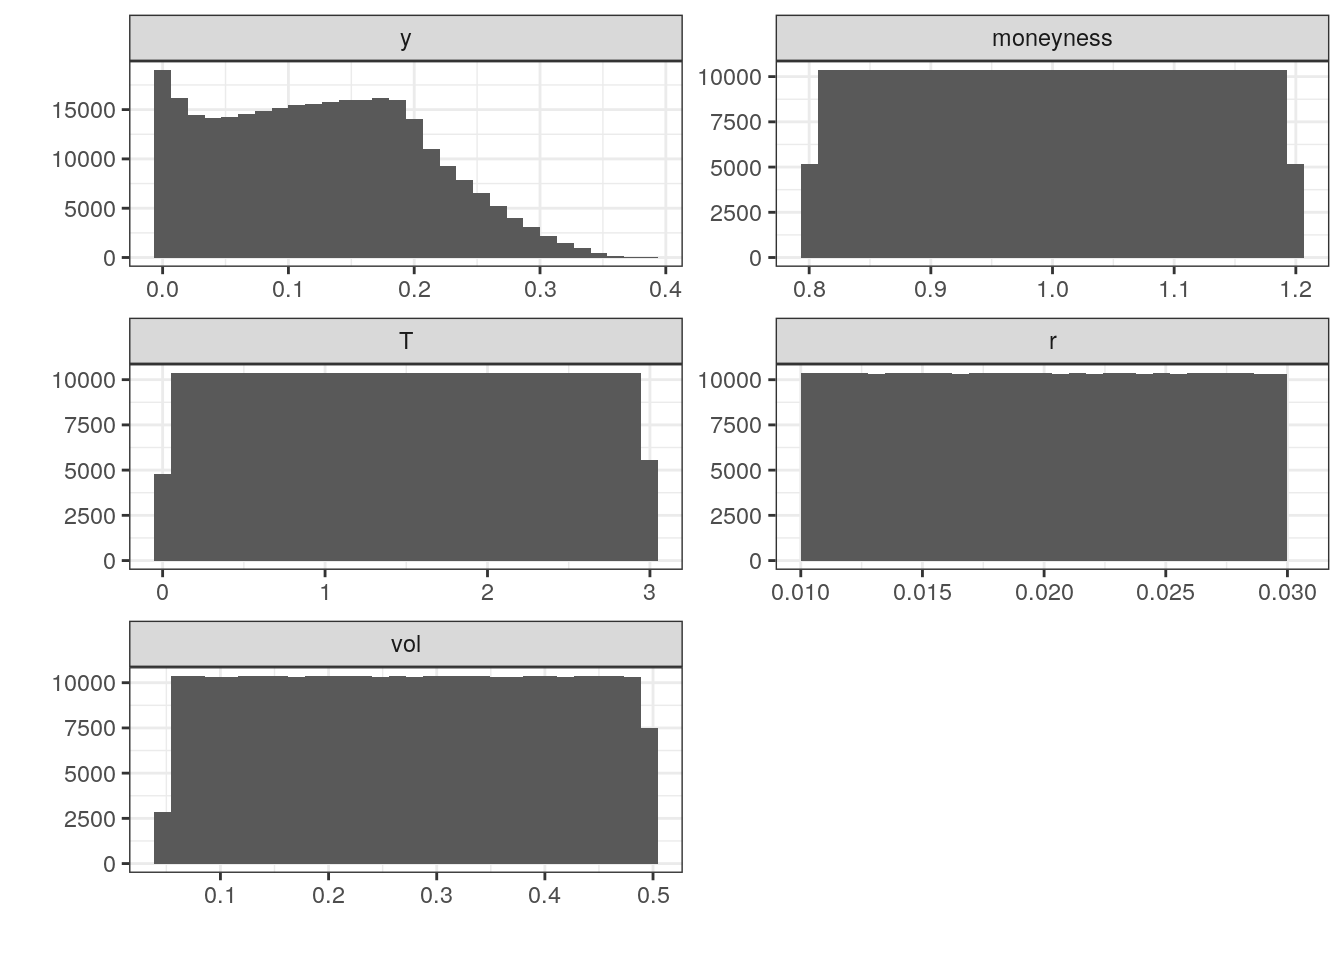
\includegraphics{Figures/marginalAmerPut.png}
\decoRule
\caption[Marginal Distributions for American Put]{Quasi random simulation with Halton sequences for input variables and CRR for generation of labels for American put option.}
\label{fig:marginalAmerPut}
\end{figure}

In figure \ref{fig:marginalAmerPut} we have visualized a simulated training data set for the American put. The marginal distributions shown is for $300.000$ data samples ($\matr{X},y$) generated by Halton sequences and the CRR model. The marginal distributions for the features cover the parameter range almost uniformly and the simulated y lies with most values at zero and maximum at 0.387 rounded to three decimals. The marginal distributions show that we have successfully generated parameters in the given ranges and the parameters are evenly spaced in the ranges. In the model performance section the out-of-sample and in-sample test data sets will be used to check the extrapolation and interpolation of the models. The test data sets are 60.000 generated data points with uniform sampling.

%-----------------------------------
%	SUBSECTION 2
%-----------------------------------

\subsection{Training}\label{Training}
The aim of training is that the model will learn the pricing function $f^*$. Once the data set ($\matr{X}, \bm{y}$) is generated the model can be trained to approximate the true function $f^*$. We will also present a standard linear model to compare the MLP with. We want to have a fast, robust, and accurate model after training on the training set. To train the model we need a measure for the error, where the mean squared error (MSE) for regression is applied. I.e. the cost function is chosen to be the empirical risk function with a quadratic loss function:
$$J(\theta)= \frac{1}{K} \sum_{k=1}^{K}(y_k-\hat{y}_k)^2$$
The MSE penalizes outliers stronger than, e.g. mean absolute error (MAE), but it penalizes small deviations less. To avoid overfitting we regularize using early stopping with a patient of 5 epochs, but with a maximum of 100 epochs for computational reasons. To update the weights the Adam optimization algorithm is chosen.  The learning rate $\eta$ is found by hyperparameter tuning for the American put minimum on two assets option and chosen to be 0.001 for the univariate contingent claims.\\

\subsubsection{Hyperparameter Tuning}
A research area within deep learning is to fine-tune the hyperparameters to the specific task, where both manually and automated searches can be used. To choose the best hyperparameters there are several choices, where the most basic automated task is random search and grid search. The random search is to define a predefined range to pick randomly from. This method can be effective to discover new hyperparameter values or combination, but it can be considerably more computationally expensive than the grid search. The grid search is used for searching in a grid with each hyperparameter in each dimension. The grid search has fast computational time relative to the random search, but requires some expert knowledge about the hyperparameters.\\

We test empirically the best hyperparameters for the MLP, where the validation set is used. For hyperparameter tuning grid search is conducted to find the optimal set of hyperparameters, where we will look at data set size, learning rate, and batch size. \\

Firstly, the European call option regression is investigated, where we vary the data set size and batch size. The goal is to quantify how large a data set($d$) and batch size($b$) are needed for having a high quality model for the European option. The data sets for an European call option considered are in-sample data sets of size 1K, 10K, 100K, 300k and 1M data samples, where the validation set is subsampled from the training data set. The batch sizes are 64, 256 and 1024, i.e. we have the combinations expressed by the Cartesian product:
$$b \times d = \{(b, d) : b \in \{64, 256, 1024\} \ and \ d \in\{1K,10K,100K,300K,1M \} \}$$
By inspiration from \parencite{HirsaAli2019} we train a MLP model with 4 layers, 120 neurons in each hidden layer and 1 neuron in the output layer. In each layer we choose the activation function leaky ReLU with negative slope $\alpha$=0.01, which is one of the most popular choices for activation functions. The number of data samples is relevant for real data, because for real market data there is not unlimited market data available.\\

\begin{table}[th]
\caption{Grid Search for European Call}{Hyperparameter tuning of data set size and batch size for the European call option. The table shows validation loss in ascending order for different hyperparameter combinations and for the interested reader the tensorboard is online (link \href{https://tensorboard.dev/experiment/8pxUoSDmTVGMOxpJWgiZsA/}{tensorboard 1})}
\label{tab:hyperEuroC1}
\centering
\begin{tabular}{lllll}
\toprule
\textbf{Data set Size} & \textbf{Batch Size} & \textbf{Training Loss} & \textbf{Validation Loss} & \textbf{Time: min:sec}\\
\midrule
1M    & 256   & $8.094\cdot 10^{-7}$ & $8.7764\cdot 10^{-7}$ & 3:38 \\ 
300K  & 64    & $7.0562\cdot 10^{-7}$ & $1.0849\cdot 10^{-6}$ & 2:49 \\ 
1M    & 1024  & $1.1596\cdot 10^{-6}$ & $1.1578\cdot 10^{-6}$ & 5:58 \\ 
300K  & 256   & $9.579\cdot 10^{-7}$ & $1.3268\cdot 10^{-6}$ & 2:29 \\ 
300K  & 1024  & $1.5367\cdot 10^{-6}$ & $1.4138\cdot 10^{-6}$ & 9:28 \\ 
1M   & 64    & $3.4919\cdot 10^{-7}$ & $1.9197\cdot 10^{-6}$ & 8:24\\ 
100K  & 256   & $2.243\cdot 10^{-6}$ & $2.1192\cdot 10^{-6}$ & 1:02  \\ 
100K  & 64    & $1.9565\cdot 10^{-6}$ & $2.5738\cdot 10^{-6}$ & 1:01 \\ 
100K  & 1024  & $3.22\cdot 10^{-6}$ & $4.4754\cdot 10^{-6}$ & 2:00\\ 
10K  & 256   & $1.1179\cdot 10^{-5}$ & $1.0980\cdot 10^{-5}$ & 0:37 \\ 
10K   & 64    & $1.0043\cdot 10^{-5}$ & $1.9830\cdot 10^{-5}$ & 0:15 \\ 
1K   & 64    & $6.1389\cdot 10^{-5}$ & $7.8711\cdot 10^{-5}$ & 0:22\\ 
10K   & 1024 & $8.7067\cdot 10^{-5}$ & $8.1122\cdot 10^{-5}$ & 0:32  \\ 
1K   & 256   & $1.2032\cdot 10^{-4}$ & $1.2504\cdot 10^{-4}$ & 0:20    \\ 
1K    & 1024  & $7.5948\cdot 10^{-3}$ & $7.3595\cdot 10^{-3}$ & 0:08    \\ 
\bottomrule\\
\end{tabular}
\end{table}

Table \ref{tab:hyperEuroC1} shows that the the model performs well for in-sample data with 10K-300K data points. The biggest data set with 1M seems not to be worth the computational cost. The model is only trained once on each data sets, so there is some randomness on each run. The model to interpolate prices for European call options in-sample data does not significantly improve with gathering more data than 10K-300K data points, which is good news for using the method on real market data.  Beware that the simulated data can underestimate the validation error, because we have a controlled setup where the parameter range is within a predetermined range. For the controlled setup with simulated data we can choose arbitrary many data points, albeit making the method more computationally expensive. By weighting both the computational cost and accuracy, we choose to work with 300K data points and a batch size of 64 for the European option. \\

The European option needs fewer parameters compared to the American put on minimum of two assets, hence, the data set might need to be larger for that study. We conduct a large grid search with variations of the learning rate $\eta$, the batch size $b$ and the data set size $d$, where the grid of the Cartesian product of $\eta$, $b$ and $d$ is searched.
$$\eta \times b \times d = \{(\eta,b, d) : \eta \in \{0.0001, 0.001, 0.01 \}, \ b \in \{8, 64, 256, 512, 1024\} \ and \ d \in\{1K,100K,300K \} \}$$
Besides varying the hyperparameters for $\eta$, $b$ and $d$, the other hyperparameters are the same values as for the European call option.\\

\begin{table}[th]
\caption{Grid Search for American Put Minimum on two Stocks}{Hyperparameter tuning of data set size, learning rate and batch size for the American put bivariate contingent claim. The table shows the top 10 best performing combinations for the training loss and for the interested reader the tensorboard is online (link \href{https://tensorboard.dev/experiment/ECWCP8nPTJWoXKVdBcQSaw/#scalars}{tensorboard 2}) and the full table is given in appendix table \ref{tab:fullhyperAmerMin4}}
\label{tab:hyperAmerMin1}
\centering
\begin{tabular}{llllll}
\toprule
\textbf{Data set Size} & \textbf{Learning Rate} & \textbf{Batch Size} & \textbf{Train Loss} & \textbf{Val. Loss} & \textbf{Time: min:sec} \\
\midrule
300K     & 0.0001 & 64    & $1.350 \cdot 10^{-6}$   & $2.287 \cdot 10^{-6}$ & 4:50 \\ 
300K     & 0.001 & 64     & $2.170 \cdot 10^{-6}$   & $1.633 \cdot 10^{-6}$ & 2:13 \\ 
300K     & 0.0001 & 8     & $2.734 \cdot 10^{-6}$   & $2.638 \cdot 10^{-6}$ & 6:17\\ 
300K     & 0.0001 & 256   & $2.943 \cdot 10^{-6}$   & $2.850 \cdot 10^{-6}$ & 4:04\\ 
300K     & 0.001 & 256    & $3.685 \cdot 10^{-6}$   & $3.335 \cdot 10^{-6}$ & 1:26\\ 
100K     & 0.0001 & 64    & $4.081 \cdot 10^{-6}$   & $3.575 \cdot 10^{-6}$ & 1:44\\ 
100K     & 0.001 & 64     & $4.817 \cdot 10^{-6}$   & $5.615 \cdot 10^{-6}$ & 0:57\\ 
100K     & 0.0001 & 256   & $5.182 \cdot 10^{-6}$   & $6.367 \cdot 10^{-6}$ & 1:52\\ 
300K     & 0.0001 & 1024  & $5.534 \cdot 10^{-6}$   & $6.473 \cdot 10^{-6}$ & 3:42\\ 
300K     & 0.001 & 8      & $5.798 \cdot 10^{-6}$   & $4.284 \cdot 10^{-6}$ & 5:40\\ 
\bottomrule\\
\end{tabular}
\end{table}

Looking at table \ref{tab:hyperAmerMin1} the best configuration for the training loss is for $(\eta=0.0001, b=64, d=300K)$, where the best configuration in terms of validation loss is $(\eta=0.001, b=64, d=300K)$. The computational burden increases when training with a bigger data set, smaller learning rate, and smaller batch sizes. The learning rate effects the computational speed because we are training with early stopping regularization. The batch size effects also the computational speed, since a high batch size gives fewer iterations per epoch. Overall the data set with 300K performed best, which is expected, since a bigger data set gives more learning opportunities. Considering computational cost and the loss; the 300K data sets, the learning rate $\eta=0.001$ and a batch size of 64 are preferred.\\

Hyperparameter tuning is highly computationally expensive and there are many combinations to test out. With grid search we have seen a possible optimal choice for the learning rate, batch size, and data set size for the European call option and American put minimum on two assets. The American put option uses the same parameters as the European option, therefore,  we choose the same hyperparameters for the univariate contingent claims. Below, we will try a different model than MLP to see if we really need deep learning for this method. 

\subsubsection{Polynomial Regression}
To compare MLP and Polynomial regression the data set and the performance metrics are the same, but the model training is obviously different. The chosen data set size is with 300.000 samples and the performance metric is MSE. For simplicity the European call option is investigated, where we fit polynomials up to degree 6 for comparison of the model capacity and fit.  
$$y_i=\beta_0 + \beta_1 \cdot x_i + \cdots + \beta_n \cdot x_i^n + \epsilon_i \quad where \ n=1,2,\ldots,6$$
Plotting the fit actual vs predicted target variable (figure \ref{fig:PolynomialEuroC}), it is clear that the in-sample fit improves with the increased model capacity. The linear regression is too simple for pricing European option, but the 6 order polynomial actually performs better than the MLP for the in-sample validation set (table \ref{tab:euroPerformance}). Keep in mind that we do not only want good interpolation, but we also want good extrapolation for our fitted model. The out-of-sample data will reveal if the high order polynomial or MLP have overfitted the data.\\

\begin{figure}[H]
\centering
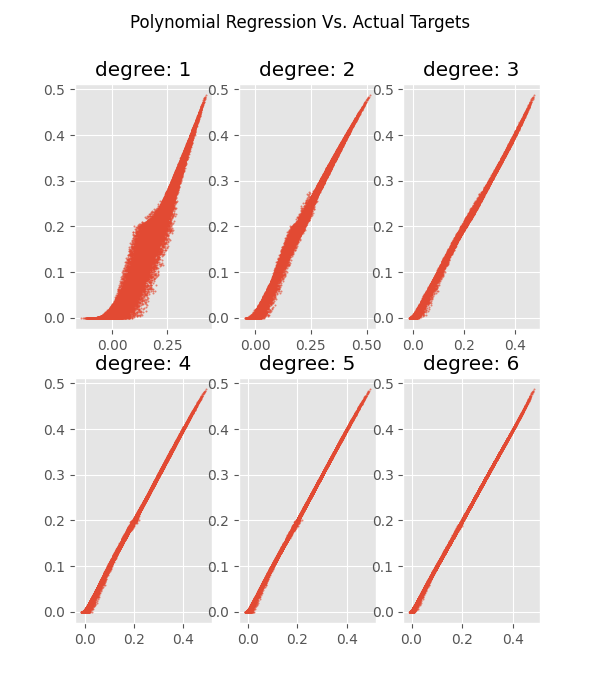
\includegraphics{Figures/polynomialEuroC.png}
\decoRule
\caption[Polynomial Regression Predictions Vs. Actual Prices]{Predicted price based on polynomial regression of varying degree}
\label{fig:PolynomialEuroC}
\end{figure}

\begin{table}[th]
\caption{European Call Validation Error}{Validation error of polynomial regression and MLP for the European call option}
\label{tab:euroPerformance}
\centering
\begin{tabular}{l l}
\toprule
\textbf{Model} & \textbf{Valalidation Loss} \\
\midrule
1. degree  poly. & 0.000631 \\
2. degree  poly.  & 0.000069 \\
3. degree poly & 0.000013\\
4. degree poly.  & 0.000004 \\
5. degree poly.  & 0.000002 \\
6. degree poly. & 0.000001\\
MLP        & 0.000003\\
\bottomrule\\
\end{tabular}
\end{table}
Looking closer at table \ref{tab:euroPerformance} to compare the performance of each model. The table confirms that the linear regression has a worse fit than the other models with higher capacity. The difference on the MLP and best performing polynomial model are less than $2\cdot 10^{-6}$. The difference is almost negligible, so the fit for MLP and polynomial regression of degree 4-6 all perform well on the in-sample training data in terms of the validation loss.

%-----------------------------------
%	SUBSECTION 3
%-----------------------------------
\subsection{Performance}
The model performance is evaluated by MSE, RMSE, MAE and coefficient of determination, where all the measures evaluate how close the model predictions are with the actual targets. The first three measure ranges are $\mathbb{R}^+$, where the goal is to have the lowest value possible. MSE close to 0 means that the model predictions do not differ a lot from the observed targets. The RMSE and MAE are the same type of measure, but the deviation is measured slightly different. The coefficient of determination has range $(-\infty, 1]$, where a higher value indicates a better model. Coefficient of determination provides a measure of how well observed targets are predicted by the model based on the proportion of total variation of targets explained by the model.

\subsubsection{European Call Option}
The European call option is trained with the algorithm and hyperparameters described in the training section (section \ref{Training}). By the hyperparameter investigation we choose a batch size of 64 and a data set of 300K samples. We compare the MLP regression with the polynomial regression. Table \ref{tab:ComparePolyWithMLP} shows that the MLP is superior at extrapolating, because the MLP performs better on all metrics on the out-of-sample test data sets compared to fitted polynomial regressions with a degree between 1 and 6\footnote{The out-of-sample fits for the European call with polynomial regression are illustated in figure \ref{fig:MLPEuroCOutOfMoney} and figure \ref{fig:MLPEuroCLongMaturity}}. For the in-sample test data set the polynomial regression of order 6 and MLP perform almost equally well. Note, the in-sample test data is similar to the in-sample training data, hence, we expect the same magnitude of error for the test set as for the training set for in-sample testing. The performance measures show that the polynomial regression, that was performing well on the in-sample data set, was due to overfitting, because the high order polynomial regression performs poorly on out-of-sample data (table \ref{tab:ComparePolyWithMLP}). For the 6. order polynomial regression, we see a negative coefficient of determination, which means the model performs worse than the model that predicts the sample mean. \\

\begin{table}[H]
\caption{Test Error for European Call Option}{Performance comparison of MLP and polynomial regression for the European call option. Shown the best performing regressions in the linear model and the worst performing in terms of MSE for in-sample and out-of-sample test data sets (The full table for polynomial regression is found in appendix table \ref{tab:fullEuroCall})}
\label{tab:ComparePolyWithMLP}
\centering
\begin{tabular}{l l l l l l l }
\toprule
\textbf{Model} & \textbf{Data set} & \textbf{MSE} & \textbf{RMSE} & \textbf{MAE} & \textbf{Coefficent of Determination} \\
\midrule
MLP & In-Sample & 0.000000 & 0.000629 & 0.000486 & 0.999961\\
& Out-of-Money & 0.000007 & 0.002644 & 0.001551 & 0.995911\\
& Long Matuiry & 0.000197 & 0.014048 & 0.010061 & 0.986518\\
6. degree poly. & In-Sample & 0.000001 & 0.000958 & 0.000591 & 0.999909\\
1. degree poly. &  & 0.000636 & 0.025212 & 0.018326 & 0.936628\\
2. degree poly. & Long Maturity & 0.001196 & 0.034577 & 0.026287 & 0.918316\\
6. degree poly. &  & 0.043361 & 0.208233 & 0.111190 & -1.962442\\
2. degree poly. & Out-Of-Money & 0.000767 & 0.027694 & 0.022203 & 0.551246\\
1. degree poly. &  & 0.005772 & 0.075973 & 0.060936 & -2.377251\\
\bottomrule\\
\end{tabular}
\end{table}

The MLP has high predictive strength compared to the polynomials, because it performs well, also on out-of-sample data sets. The MLP show that it predicts out-of-money call options with less than a MSE value of $10^{-5}$, where the fit for the long maturity test set has a higher MSE. The European options are liquid in the markets, hence, the pricing method can easily be trained on real data. The MLP fit for in-sample data on the European call option is visualized in figure \ref{fig:MLPInSampleEuroC}, which shows $\frac{c(S_0,K)}{K}$ predicted from the model and observed target values $\bm{y}$. The figure shows a overall close fit. For the remaining part of this section only the MLP regression will be considered, because the polynomial regression has shown bad performance for out-of-sample data.

\begin{figure}[th]
\centering
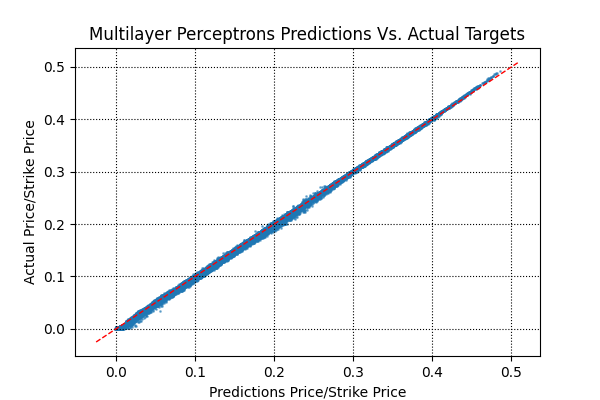
\includegraphics{Figures/PredictionEuroC.png}
\decoRule
\caption[MLP Performance for In-sample Dataset European Call]{MLP Performance on in-sample dataset on European call}
\label{fig:MLPInSampleEuroC}
\end{figure}


\subsubsection{American Put Option}
The American put option is priced with the same MLP algorithm as for the European call. Table \ref{tab:AmerPerformanceComparision} shows once again a good fit, hence, we believe we have a high quality model for the American put option\footnote{The out-of-sample fits for the American put with MLP regression are illustated in figure \ref{fig:MLPAmerPOutMoney} and figure \ref{fig:MLPAmerPLongT}}.

\begin{table}[th]
\caption{MLP Performance on American Put Option}
\label{tab:AmerPerformanceComparision}
\centering
\begin{tabular}{l l l l l l l }
\toprule
\textbf{Data set} & \textbf{MSE} & \textbf{RMSE} & \textbf{MAE} & \textbf{$R^2$} \\
\midrule
In-Sample & 0.000002 & 0.001562 & 0.001278 & 0.999634\\
In-The-Money & 0.000012 & 0.003519 & 0.002290 & 0.995778\\
Longer Maturity & 0.000193 & 0.013894 & 0.009213 & 0.980835\\
\bottomrule\\
\end{tabular}
\end{table}

\subsubsection{American Put on Minimum of two Assets Option}
The American put on minimum of two assets option has almost double the number of parameters compared to the univariate contingent claims. Hence, the performance might produce a slightly higher MSE. Table \ref{tab:AmerMinPerformanceComparision} and figure \ref{fig:MLPInSampleAmerMin} show that the MLP also fits the American put minimum option on two assets well. The performance seems similar to the univariate case, hence we see that the MLP can easily fit bivariate contingent claims as well. \\ 

\begin{table}[th]
\caption{Performance of the Bivariate American Put Contingent Claim}
\label{tab:AmerMinPerformanceComparision}
\centering
\begin{tabular}{l l l l l l l }
\toprule
\textbf{Data set} & \textbf{MSE} & \textbf{RMSE} & \textbf{MAE} & \textbf{$R^2$} \\
\midrule
In-Sample & 0.000002 & 0.001361 & 0.001008 & 0.999794\\
In-The-Money & 0.000143 & 0.011973 & 0.009208 & 0.964370\\
Longer Maturity & 0.000112 & 0.010565 & 0.007319 & 0.989863\\
\bottomrule\\
\end{tabular}
\end{table}

\begin{figure}[H]
\centering
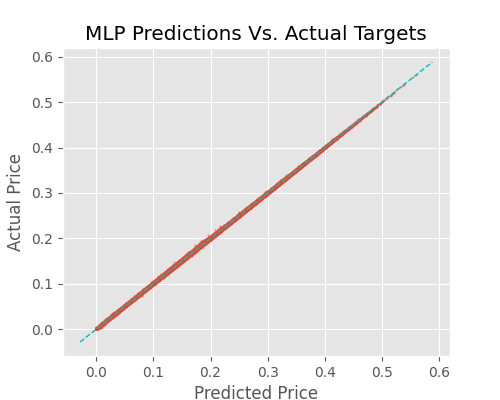
\includegraphics{Figures/inSampleAmerMinP.png}
\decoRule
\caption[MLP Performance for In-sample Dataset American Put on minimum on two Assets]{MLP Performance on in-sample dataset on American bivariate contingent claim}
\label{fig:MLPInSampleAmerMin}
\end{figure}

The MLP has shown good performance in terms of our performance measures on all the derivatives considered. Next chapter will compare this MLP model (henceforth referred to as MLP II) with the closed form solutions, binomial model, LSM and LSM MLP (henceforth referred to as MLP I). All the models considered in this section had good performances on the in-sample dataset except for the too simple models; linear regression and 2. degree polynomial regression. The MLP II was superior for out-of-sample data sets compared to the polynomial regression in terms of our performance measures.\\

The MLP II is not based on a model, it is only trained on the available data. This feature makes the MLP II pricing method versatile, because the MLP could also be used for actual market data or different models to learn patterns. The fact that the method can be extended to real market data is already shown in \parencite{GasparRaquel20}. This section showed how the MLP can be trained to pricing derivatives with Black-Scholes theory and that the MLP is preferred over polynomial regression.









 
% Chapter Template

\chapter{Numerical Investigation and Discussion} % Main chapter title

\label{Chapter6} % Change X to a consecutive number; for referencing this chapter elsewhere, use \ref{ChapterX}

This chapter will empirically compare the numerical and analytical methods presented for different types of contingent claims\footnote{The interested reader can see the implementation details in appendix \ref{AppendixD}}. The underlying model will be the Black-Scholes model, because it has closed form solutions for some European options and is thoroughly researched.\\

We look at the closed form solutions to the European options compared with the binomial lattice model for pricing. The closed form solution provides a measure of how the binomial lattice model approximates European options in the Black-Scholes model. The binomial model is readily extended to American options, hence, the section also gives an indication of how the binomial model approximates the American option. The American put option is then investigated, where the different numerical methods considered are compared. The last type of option we look at is the American put minimum on two stocks option. After the numerical investigation the pricing methods and model assumptions are discussed.


%----------------------------------------------------------------------------------------
%	SECTION 1
%----------------------------------------------------------------------------------------
\section{European Options}\label{EuroOption}
European options are simple in the sense, that they can only be exercised at maturity. Throughout the previous chapters, especially chapter \ref{Chapter2} and \ref{Chapter3}, we have seen closed form solutions for the simple European and exotic European options. The binomial lattice models presented are models that can approximate European options and American options. The closed form solutions and the binomial lattice approach can be compared for European options, where a small deviation between methods for the European options indicates that the lattice approach gives reasonable prices for the American options.\\

The simplest case is the European call option, where we look at how the CRR model and the MLP II pricing model approximate the B-S call formula. Table \ref{tab:EuroCall} empirically shows that the CRR model price prediction converges toward the price from the Black-Scholes call formula, which is in line with the theoretical result for the CRR model that it converges to the Black-Scholes model. The MLP II pricing method underprices the European call option, but it performs better for this example than the CRR with 10 and 30 time-steps. Keep in mind we trained the MLP II with the CRR 100 equidistant time-steps model, therefore, we might have seen a better fit with a data set generated with $10^4$ time-steps.\\

\begin{table}[th]
\caption{CRR, MLP II, and B-S Call Formula Comparison}{Comparison of accuracy for the European call option, where the inputs are K=40, $S(0)=40$, $\sigma=0.2$, T=1, and r=0.06.}\\
\label{tab:EuroCall}
\centering
\begin{tabular}{l l l}
\toprule
\textbf{Method} & \textbf{No. Steps} & \textbf{Price} \\
\midrule
CRR & 10 & 4.316\\
& 30 & 4.369\\
& 50 & 	4.380\\
& 100 & 4.388\\
& 200 & 4.392\\
& 500 & 4.394\\
& 1000 & 4.395\\
& 10000 & 4.396\\
MLP II & & 4.370\\
Analytic form & & 4.396\\
\bottomrule\\
\end{tabular}
\end{table}

The natural extension of the CRR model is the BEG model, where it is possible to price more exotic options. Section \ref{ExoticEuro} showed some closed form solutions for exotic European options. Hence, we have a benchmark for the BEG in these special cases. We choose to look at the computation time for European put minimum with two underlying assets, which has a closed form solution. Closed form solutions make it easy to look at the trade-off between accuracy and computational cost for the BEG method. \\

\begin{table}[th]
\caption{BEG Accuracy and Speed}{Comparison of speed and accuracy for a European put min option, where the inputs are K=40, $S_1(0)=S_2(0)=40$, $\sigma_1=0.2, \sigma_2=0.3$, T=1, $\rho=0.5$,  and r=0.06. Note ms is shorthand for millisecond}
\label{tab:TradeOffEuroMin}
\centering
\begin{tabular}{l l l l}
\toprule
\textbf{Method} & \textbf{No. Steps} & \textbf{Price} & \textbf{Time: min:sec.ms} \\
\midrule
BEG & 10 & 4.248 & 0:00.003\\
& 50 & 4.341 & 0:00:097\\
& 100 & 4.352 & 0:00.591\\
& 200 & 4.358 & 0:04.121\\
& 500 & 4.361 & 0:59.337\\
& 1000 & 4.362 & 9:34.164\\
Analytic form & & 4.363 & \\
\bottomrule\\
\end{tabular}
\end{table}
Tabel \ref{tab:TradeOffEuroMin} shows that the algorithm accuracy increases with the number of equidistant time-steps, but the computational speed dramatically slows down when the time-steps increases. Therefore, for exotic options the computational costs become a factor to consider\footnote{Note the implementation is written in Python, hence, the code can be improved in terms of computational efficiency. The computations are performed on my laptop with 8GB ram and 8th Generation Intel® Core™ i5 processor}. The BEG method accuracy is also tested on the European call minimum and European call maximum for 100 time-steps, where the BEG method is within 0.13 of the analytic solution (table \ref{tab:PriceEuropean}).\\
\begin{table}[th]
\caption{BEG and Exotic European Options}{Valuation of bivariate contingent claims with K=40, $S_1(0)=S_2(0)=40$, $\sigma_1=0.2, \sigma_2=0.3$, T=1, $\rho=0.5$,  and r=0.06.}
\label{tab:PriceEuropean}
\centering
\begin{tabular}{l l l l}
\toprule
\textbf{Derivative type} & \textbf{Method} & \textbf{No. Steps} & \textbf{Price} \\
\midrule
European Call Minimum & BEG & 100 & 2.475\\
& Analytic form & & 2.483\\
European Call Maximum & BEG & 100 & 7.787\\
& Analytic form & & 7.800\\
\bottomrule\\
\end{tabular}
\end{table}
 
The above tables show that the binomial pricing model can be used for both univariate and bivariate European contingent claims. The binomial model accuracy is high for European options, hence, we expect a similar good approximation for the American option. The CRR for univariate and BEG for bivariate contingent claims will be used as benchmarks for the American options, where we investigate LSM, MLP I and MLP II pricing methods. \\

Note that the BEG is not practical for pricing multivariate contingent claims with many underlying assets, because the possible states for the stochastic processes increase exponentially. Therefore, the bivariate contingent claim is considered instead of higher dimensional basket options in section \ref{bivariateAmerPut}.
%----------------------------------------------------------------------------------------
%	SECTION 2
%----------------------------------------------------------------------------------------
\section{American Put Option}
The American put option has no analytical solution in the Black-Scholes model, thus, numerical methods are required. We present and compare the results for the LSM, MLP I and MLP II pricing methods compared to the CRR model.\\

The LSM and MLP I pricing method are almost identical, except the MLP tries to utilize deep learning to regress the expected continuation value. Both pricing methods converge to the optimal value process\footnote{See appendix \ref{Convergence}}, hence, we numerically expect that by increasing the computational burden we approach the true price. To compare the two methods we simulate $10^5$ paths for the stock under the assumption that the future price of the stock is lognormal. The LSM and MLP I pricing methods are used on the same simulated paths, but produce a different result each time due to the Monte Carlo simulations. The CRR and MLP II\footnote{Note that we talk about the model after training} are not random in the sense that the output is deterministic, because both approaches do not involve Monte Carlo simulation. For the LSM and MLP I we assume 50 equidistant exercise dates for each year, where for the CRR we use 1000 equidistant time-step for the stock.  \\

The MLP I requires us to set some hyperparameters, where we choose the learning rate $\eta=0.001$, batch size of 512 and the Adam optimization algorithm. The architecture of the MLP is three layers, where the hidden layers are with 40 neurons and the output layer has one neuron. The activation functions are set to Leaky ReLU with 0.3 negative slope and the trained model is reused at each decision point by inspiration from \parencite{Lelong19}. The choices are partly inspired by the work by \parencite{Lelong19} and empirical testing. The regression in the LSM is done with a polynomial regression of degree 10. Remember the MLP II is trained with the same hyperparameters as for the European call option and the CRR with 100 time-steps is used to generate labels.\\

\begin{table}[th]
\caption{Valuation of American Put Option}{We choose the fixed parameters K=40 and r=0.06}
\label{tab:AmericanPut}
\centering
\begin{tabular}{l l l l l l l }
\toprule
\textbf{Spot} & \textbf{$\sigma$} & \textbf{T} & \textbf{CRR} & \textbf{LSM} & \textbf{MLP I} & \textbf{MLP II} \\
\midrule
36 & 0.2 & 1 & 4.487 & 4.481 & 4.364 & 4.584\\
36 & 0.2 & 2 & 4.848 & 4.846 & 4.747 & 4.649\\
36 & 0.4 & 1 & 7.109 & 7.118 & 6.919 & 7.090\\
36 & 0.4 & 2 & 8.508 & 8.514 & 8.215 & 8.487\\
38 & 0.2 & 1 & 3.257 & 3.258 & 3.217 & 3.094\\
38 & 0.2 & 2 & 3.751 & 3.748 & 3.681 & 3.638\\
38 & 0.4 & 1 & 6.154 & 6.157 & 6.075 & 6.172\\
38 & 0.4 & 2 & 7.675 & 7.695 & 7.359 & 7.605\\
40 & 0.2 & 1 & 2.319 & 2.317 & 2.292 & 2.114\\
40 & 0.2 & 2 & 2.900 & 2.896 & 2.823 & 2.779\\
40 & 0.4 & 1 & 5.318 & 5.329 & 5.180 & 5.274\\
40 & 0.4 & 2 & 6.923 & 6.934 & 6.750 & 6.839\\
42 & 0.2 & 1 & 1.621 & 1.623 & 1.599 & 1.494\\
42 & 0.2 & 2 & 2.217 & 2.224 & 2.183 & 2.167\\
42 & 0.4 & 1 & 4.588 & 4.600 & 4.538 & 4.548\\
42 & 0.4 & 2 & 6.250 & 6.269 & 6.111 & 6.197\\
44 & 0.2 & 1 & 1.113 & 1.119 & 1.094 & 1.000\\
44 & 0.2 & 2 & 1.694 & 1.700 & 1.653 & 1.678\\
44 & 0.4 & 1 & 3.954 & 3.959 & 3.931 & 3.949\\
44 & 0.4 & 2 & 5.647 & 5.669 & 5.524 & 5.649\\
\bottomrule\\
\end{tabular}
\end{table}

Table \ref{tab:AmericanPut} shows that the MLP I always predicts a lower price than the LSM, therefore, for our numerical study, the LSM seems to be better than the MLP I in terms of approximating the \textsl{"true"} price. The reference is the CRR model, which is a deterministic method. The MLP II trained with the CRR model shows high deviation from the CRR predicted price compared to LSM. The total deviation in absolute distance for the MLP II is 1.56, where LSM deviation is 0.157 for the above table containing 20 prices with different unique input parameters combinations. The MLP II is, however, better in total absolute deviation compared to the MLP I, which has a total absolute deviation of 2.078. This indicates that the MLP II, at this stage of development, is preferred over the MLP I in terms of speed and accuracy. The MLP I and LSM have uncertainty from the Monte Carlo simulation and with $10^5$ paths the standard error of the means are 0.0019 and 0.0214. The standard error\footnote{Sometimes written in short form SE} of the means are calculated by 100 samples\footnote{Denoted with n in the formulas} for the input parameters T=1, $\sigma=0.4$, $r=0.06$, $S(0)=36$, and $K=40$. The empirical distribution mean is calculated by
$$\bar{x}= \frac{1}{n}\sum_{i=1}^{n} x_i$$
and the standard error of the mean
$$\sigma_{\bar{x}}= \frac{\sigma}{\sqrt{n}} \quad where \ \sigma=\sqrt{\frac{1}{n-1}\sum_{i=1}^{n} (x_i-\bar{x})}$$
 
The histogram (figure \ref{fig:histLSMMLPI}) shows the variation in the estimates where the CRR price is the dashed black line. We see that the MLP I has higher standard error than the LSM and the center of the distribution\footnote{Sample mean is 6.9048} is lower than the CRR price\footnote{CRR price is 7.1094}. The LSM, on the other hand, has less variability and the center\footnote{Sample mean is 7.1074} is around the CRR price. Hence in term of numerical stability, computational speed and accuracy the LSM is superior for the American put. The reason for the numerical instability for the MLP I is that the optimization algorithm is random on each run compared to the linear model\footnote{E.g. polynomial regression where the solution is exact and unique}.\\

\begin{figure}[H]
\centering
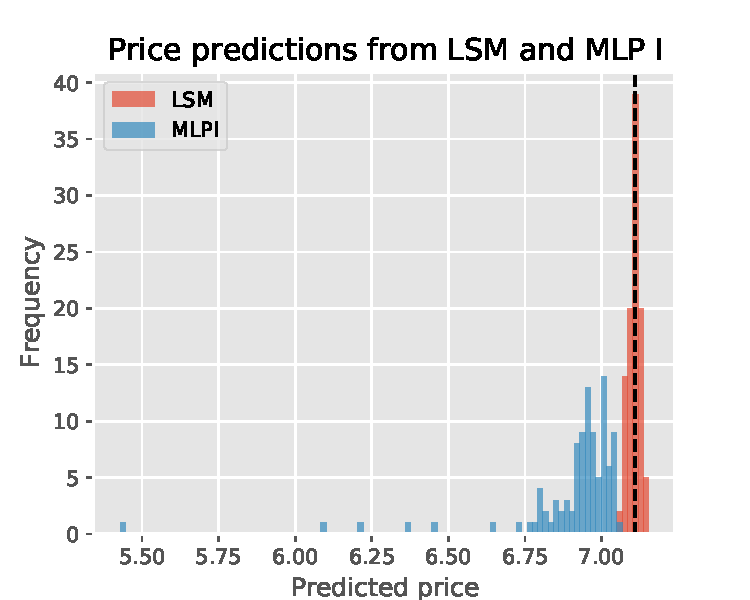
\includegraphics{Figures/histLSMMLPsI.pdf}
\decoRule
\caption[Histogram Price Predictions]{100 predicted prices for American put option with LSM and MLP I. Parameters are T=1, $\sigma=0.4$, $r=0.06$, $S(0)=36$, and $K=40$. Note CRR price is the dashed black line.}
\label{fig:histLSMMLPI}
\end{figure}

Improvements of MLP I is needed in order for the method to challenge the existing LSM, both in terms of speed and accuracy for low dimensional problem. Possible improvement of the MLP I could be conducted by a large hyperparameter tuning study. The issue with hyperparameter tuning is that it is computationally expensive. For the MLP I the hyperparameter tuning needs to be searched at every decision point. Another type of network could also be considered, e.g. recurrent neural network. The inferior results from the MLP I to the LSM show that some work still needs to be done. We choose not to consider MLP I and LSM for the next section, because of the poor results from the MLP I pricing method in this section.\\
%----------------------------------------------------------------------------------------
%	SECTION 3
%----------------------------------------------------------------------------------------
\section{American Put Minimum on two Assets Option}\label{bivariateAmerPut}
There are many exotic American options to consider, but we choose to focus on the American put minimum on two stocks option, because MLP II is trained to predict prices on this specific option. The other advantage is that we have the deterministic method BEG for the bivariate contingent claim, hence, the MLP II can easily be compared, both for accuracy and speed.\\

First, we look at the computational cost for the BEG method by increasing the number of time-steps. By looking at table \ref{tab:TradeOffAmerMin} it is clear that the computational time is dependent on the number of time-steps. We know from the discussion in section \ref{EuroOption} that the accuracy increases by increasing the number of time-steps. Weighting the computational cost and accuracy we choose to use the BEG method as reference price with 500 time-steps. Note, that when we generated the labels for the MLP II pricing method we used 50 equidistant time-steps. The reason for using 50 time-steps is that we simulated 300.000 data points, which is a computational heavy task. A MLP II model trained with 500 time-steps would probably predict the price from the BEG method with 500 steps better, but it was not computationally feasible. This creates an expectation that the option priced with MLP II will have a bias price and therefore, we will also include the BEG with 50 time-steps in the comparison.\\

\begin{table}[th]
\caption{BEG for the American Bivariate Contingent Claim}{Comparision of speed for the American put minimum on two assets option, where the inputs are K=40, $S_1(0)=S_2(0)=40$, $\sigma_1=0.2, \sigma_2=0.3$, T=1, $\rho=0.5$  and r=0.06. Note ms is shorthand for millisecond}
\label{tab:TradeOffAmerMin}
\centering
\begin{tabular}{l l l l}
\toprule
\textbf{Method} & \textbf{No. Steps} & \textbf{Price} & \textbf{Time: min:sec.ms} \\
\midrule
BEG & 10 & 4.524 & 00:00.006\\
& 50 & 4.594 & 00:00.250\\
& 100 & 4.602 & 00:01.837\\
& 200 & 4.605 & 00:14.025\\
& 500 & 4.608 & 03:35.039\\
& 1000 & 4.609 & 28:32.584\\
MLP II &  & 4.426 & 00:00.0003\\
\bottomrule\\
\end{tabular}
\end{table}

Table \ref{tab:TradeOffAmerMin} shows that the price for the American put minimum is greater than the European put minimum from table \ref{tab:TradeOffEuroMin}. Additionally, it is clear that the computational time increases for the American option, because we have to compare intrinsic value and expected continuation value at each node. Both results are good sanity checks.\\

For visualization we plot the BEG50, BEG500, and MLP II for varying spots with fixed K=40, $\sigma_1=0.2$, $\sigma_2=0.3$, T=1, $\rho=0.5$,  and r=0.06. The figure shows that the BEG500\footnote{BEG method with 500 time-steps} and BEG50 are close to each other. The total absolute deviation is 0.142 for the 21 prices, which shows that the BEG50 is suffient for training our MLP. The total absolute deviation for the MLP II with the BEG500 is 3.716 and with the BEG50 3.713. This is depicted in figure \ref{fig:BEGMLPII}, where the MLP underprices the option for the in-sample domain with varying spot. To compare the computational speed the MLP II took around 00:00.000349 to generate one price, which is considerable faster than the BEG model with 10 time-steps. Hence, we see that we loose some accuracy with the MLP II, but the pricing method is fast. 

\begin{figure}[H]
\centering
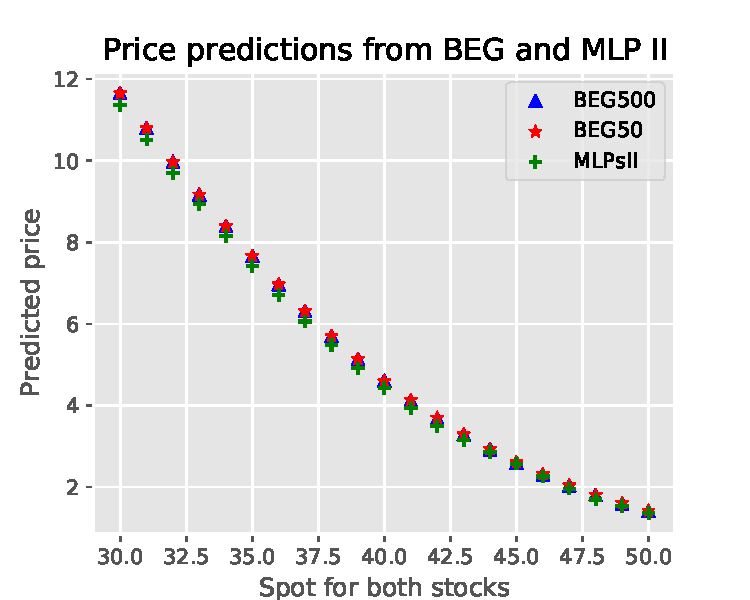
\includegraphics{Figures/compareBEGMLPsII.pdf}
\decoRule
\caption[Compare BEG and MLP II]{Scatter plot of predicted prices for American put minimum on two assets option with BEG and MLP II. Parameters are T=1, $\sigma_1=0.2$, $\sigma_2=0.3$, $r=0.06$, $K=40$ and $\rho=0.5$. Note BEG is showed for 50 time-steps and 500 time-steps.}
\label{fig:BEGMLPII}
\end{figure}

The MLP might provide a better estimate by simulating more data samples and make the model more complex, but our hyperparameter tuning study was not conclusive on this point. Hyperparameter tuning could also be further investigated, e.g. looking at depth and width of the network. The real power of pricing with MLP II is when the computational burden becomes an issue for fast pricing. 

%----------------------------------------------------------------------------------------
%	SECTION 4
%----------------------------------------------------------------------------------------
\section{Discussion of Pricing Methods}
The idea behind using neural networks instead of the linear model, is that the neural networks scale better for high dimensional problems. We have only considered univariate and bivariate contingent claims, because in these cases we have a deterministic alternative in the binomial lattice models. This gives a good indication of how the model predicts. Besides, if the model does not perform well for low dimensional problems, we would not expect the model to be any better for more complex multivariate contingent claims.\\

Remember, the binomial lattice model also has its limitations in terms of computational resources, because the computational burden scales exponentially with the number of underlying risky assets\footnote{The same can be said about the PDE methods}. The LSM is versatile and can be used for most derivatives, because it relies on Monte Carlo simulation and regression. For considering multivariate contingent claims the LSM is readily useful, but the linear model for regression suffers the curse of dimensionality for basket options with many underlying risky assets. We have in mind that a neural network does not suffer from the curse of dimensionality, hence, the method, compared to the linear model, has advantages when considering multivariate contingent claims. The idea of neural network should work in theory\footnote{Universal approximation theorem for MLP}, but the numerical results shown in this chapter are not satisfying for the MLP I in the univariate case.\\

The MLP II is somewhat better, but it still relies on existing option pricing methods or real market data. Therefore, it does not solve the curse of dimensionality for basket options with many underlying assets. The MLP II however, has the advantage of the increased speed after training, which could be beneficial in some circumstances. The MLP could also be used on real data and it is versatile enough to capture the volatility shew\footnote{Explanation below in section "Discussion of the Black-Scholes model"} for equity options. One drawback is that there should be enough data samples, which is relevant if the method is used on real market data. Another drawback is that the trained model would need to be calibrated regularly, because financial scenarios can change dramatically, e.g. the financial crisis in 2007-2009.\\

In the training phase of the neural networks the derivatives of the model parameters are used for minimizing the loss function. The derivatives are calculated efficiently with back propagation, which is important for risk management. Potentially, the neural networks can speed up the risk management of the derivative books and give real time risks. Deep learning for risk management is investigated in \parencite{AntoineSavine}. It should be mentioned, that the above-mentioned methods cannot only be used for equity options, the LSM is e.g. widely used for fixed income\footnote{E.g. Libor Market Model}.\\

The results from the MLP I were a bit discouraging, because it was inferior to the LSM. The computational cost is higher for the MLP I for low dimensional problems, hence, an accuracy on the same level as for the LSM would make it attractive to investigate for higher dimensional problems. One explanation could be wrong hyperparameters for the model, which would require a time consuming hyperparameter search. The grid search might have its shortcomings in this aspect, because it requires some knowledge about possible well-suited hyperparameters for the optimal stopping problem. A random search or Bayesian search could be beneficial in this aspect, but it would also require many computational resources.\\

The MLP II lack some precision compared to LSM for the univariate contingent claim. For the bivariate the MLP II again showed a loss of accuracy, but showed additional speed. A larger hyperparameter study could also be conducted here, a different method to generate labels or a bigger data set could have been sampled. E.g. the article \parencite{FergusonRyan2018} shows good result for an European basket option with 6 underlying assets by simulating a data set of 500M samples. 

%----------------------------------------------------------------------------------------
%	SECTION 5
%----------------------------------------------------------------------------------------
\section{Discussion of the Black-Scholes model}
For pricing we utilize the Black-Scholes theory, where we assume constant volatility, the interest rate is constant through time, and future stock prices are lognormal distributed. It is well-known that the volatility is not constant, in fact, it depends on the maturity and strike. The dependency on strike and maturity can be modeled with a volatility surface. Looking only at one dependency the implied volatility for equity options is a decreasing function of the strike over spot $\frac{K}{S(0)}$ for real data (p. 458 \parencite{Hull}). This phenomenon is known as volatility shew for equity options. \\

A possible reason for the volatility shew is that investors are more concerned with falling stock prices than rising prices, hence, the volatility is instantaneously negatively correlated with the stock price. To overcome the issue about assuming constant volatility, a model with stochastic variance can be considered. The model becomes more complex with an extra stochastic variable, where for simplicity we mention the two factor Heston model. The basic model is given by the stock follow the SDE:
$$dS(t)=\alpha S(t) dt + \sqrt{V(t)} S(t) dW_S(t)$$
And the stochastic variance process $V(t)$ is the solution to the SDE:
$$dV(t)=a(\theta - V(t))dt + \epsilon \sqrt{V(t)} dW_V(t) \quad where \ a>0,\theta>0, \epsilon>0, \ and \ V(0)>0$$
Where $W_S(t)$ and $W_V(t)$ have correlation $\rho$. The interpretation of the constants is:
\begin{enumerate}
\item[•] $\theta$ is long run average price variance
\item[•] a is the rate which $V(t)$ reverts to $\theta$
\item[•] $\epsilon$ is the volatility of the volatility
\end{enumerate} 
The implication of $\epsilon$ is that $V(t)$ is more volatile when volatility is high. The correlation between the stock and variance process is often modeled with a negative correlation. The negative correlation between the two processes displays the real market phenomenon of volatility shew for equity options, because when the stock price drops, volatility increases. Assuming stochastic volatility the Heston model overcomes the issue with volatility shew. Another model trying to solve the non-constant volatility is e.g. "Constant Elasticity of Variance model", but there are numerous others\footnote{E.g "Merton's Mixed Jump-Diffusion Model" and "Variance-Gamma Model"}. \\

The constant risk-free interest rate through time assumption can also be discussed, because the interest rate is not constant for real market behavior. We did not investigate the American call, because it coincides with the European call for positive interest rate. Today's market interest rates are negative for the Eurozone, which was probably unheard before the last decade's financial events. Therefore, the decision to assume positive constant interest rate through time is set for convenience.\\

The Black-Scholes model assumes that the underlying risky assets evolves as a GBM, where the distribution of possible stock prices at the end of any interval is lognormal. The model is convenient, because the GBM has a analytical solution\footnote{SDE does not always have a analytical solution}. If we wanted to investigate arithmetic mean basket option the Bachelier model would be more convenient, because the future stock price is normal distributed. 
\begin{equation*}
dS_i=\sigma_i dW_i
\end{equation*}
This assumption would simplify the pricing problem of arithmetic basket options, because the sum of normals provides a multivariate normal distribution. The basket option problem in the Bachelier is then essentially one dimensional. This is similar to the the geometric mean basket option for the Black-Scholes model (section \ref{GeoBasket}). A disadvantage with the Bachelier model is that it can lead to negative stock values, which is not realistic.\\

The Black-Scholes model has some drawbacks where you can question the assumptions, but the model is convenient to use for comparison of pricing methods. By above discussion, we stress that we do not necessarily believe that the Black-Scholes model is the true model for real market behavior. The purpose is rather to investigate pricing methods in a convenient model.


% Chapter Template

\chapter{Conclusion and Further Investigation} % Main chapter title

\label{Chapter7} % Change X to a consecutive number; for referencing this chapter elsewhere, use \ref{ChapterX}

%----------------------------------------------------------------------------------------
%	SECTION 1
%----------------------------------------------------------------------------------------

\section{Conclusion}
We have seen different methods for pricing equity options within the Black-Scholes world. We have specifically focused on the European call, exotic European, American put and American put minimum on two stocks options. The closed form solutions, the classical binomial lattice model and LSM were provided for investigating the potential of using deep learning in option pricing theory. \\

The numerical investigation showed that MLP I and MLP II pricing methods were inferior in accuracy for univariate and bivariate contingent claims, but the MLP II had an enhanced speed compared to the classical methods after training. The results for the MLP I were somewhat discouraging, but the theory tells us that we can improve our training algorithm to perform on the same level as LSM. The CRR model was extended to the BEG method with two underlying stocks, which we saw provided a good approximation for European bivariate contingent claims. The BEG method has its limitations in terms of pricing a basket option with many underlying stocks, which can be solved with LSM or MLP I.\\

To sum up, the MLP I needs hyperparameter tuning, but the underlying theory and idea gives hope for finding a better model for high dimensional data than the classical LSM. The BEG has its limitation in high dimensions. Hence, LSM is preferred for higher dimensions. The MLP II showed better performance than for polynomial regression at supervised learning. Furthermore, the MLP II can be beneficial in terms of computational speed, but has lower precision for univariate contingent claims than the LSM, compared to our CRR benchmark price.\\

The classical methods approximate the true price in the Black-Scholes model well. The deep learning methods lack the accuracy of the classical methods in the Black-Scholes model, hence, there is still some work to be done for pricing derivatives with deep learning. 

%-----------------------------------
%	SECTION 2
%-----------------------------------
\section{Further Investigation}
The code library is written in Python, which could be optimized in terms of computational speed with e.g. Julia or C++. The advantage of Python is the libraries for machine learning and especially deep learning. The code could also be more generalized, not only to handle specific option contracts by using the object oriented programming paradigm instead of procedural programming approach. The code was run on my CPU, but the speed could also be improved by using the GPU.\\

Hyperparameter tuning for the MLP would be interesting to investigate further with e.g. the more advanced method; Bayesian hyperparameter tuning. The article from \parencite{liaw2018tune} looks at how hyperparameter tuning can be easy implemented, which is worth looking at. The data sets could have been bigger or the labels could have been generated with a different method. Another interesting aspect to investigate is calculating the derivatives of the pricing function, which produces the risks for the derivative books. It looks like MLP models are superior for calculating risks in terms of speed to the classical methods, hence, there is potentially an additional gain when using deep learning.\\



%% Chapter

\chapter{Introduction} % Main chapter title

\label{Chapterinfo} % For referencing the chapter elsewhere, use \ref{Chapter1} 

%----------------------------------------------------------------------------------------

% Define some commands to keep the formatting separated from the content 
\newcommand{\keyword}[1]{\textbf{#1}}
\newcommand{\tabhead}[1]{\textbf{#1}}
\newcommand{\code}[1]{\texttt{#1}}
\newcommand{\file}[1]{\texttt{\bfseries#1}}
\newcommand{\option}[1]{\texttt{\itshape#1}}

%----------------------------------------------------------------------------------------


\section{Welcome and Thank You}
Welcome to this \LaTeX{} Thesis Template, a beautiful and easy to use template for writing a thesis using the \LaTeX{} typesetting system.

If you are writing a thesis (or will be in the future) and its subject is technical or mathematical (though it doesn't have to be), then creating it in \LaTeX{} is highly recommended as a way to make sure you can just get down to the essential writing without having to worry over formatting or wasting time arguing with your word processor.

\LaTeX{} is easily able to professionally typeset documents that run to hundreds or thousands of pages long. With simple mark-up commands, it automatically sets out the table of contents, margins, page headers and footers and keeps the formatting consistent and beautiful. One of its main strengths is the way it can easily typeset mathematics, even \emph{heavy} mathematics. Even if those equations are the most horribly twisted and most difficult mathematical problems that can only be solved on a super-computer, you can at least count on \LaTeX{} to make them look stunning.

%----------------------------------------------------------------------------------------

\section{Learning \LaTeX{}}
\LaTeX{} is not a \textsc{wysiwyg} (What You See is What You Get) program, unlike word processors such as Microsoft Word or Apple's Pages. Instead, a document written for \LaTeX{} is actually a simple, plain text file that contains \emph{no formatting}. You tell \LaTeX{} how you want the formatting in the finished document by writing in simple commands amongst the text, for example, if I want to use \emph{italic text for emphasis}, I write the \verb|\emph{text}| command and put the text I want in italics in between the curly braces. This means that \LaTeX{} is a \enquote{mark-up} language, very much like HTML.

\subsection{A (not so short) Introduction to \LaTeX{}}

If you are new to \LaTeX{}, there is a very good eBook -- freely available online as a PDF file -- called, \enquote{The Not So Short Introduction to \LaTeX{}}. The book's title is typically shortened to just \emph{lshort}. You can download the latest version (as it is occasionally updated) from here:
\url{http://www.ctan.org/tex-archive/info/lshort/english/lshort.pdf}

It is also available in several other languages. Find yours from the list on this page: \url{http://www.ctan.org/tex-archive/info/lshort/}

It is recommended to take a little time out to learn how to use \LaTeX{} by creating several, small `test' documents, or having a close look at several templates on:\\ 
\url{http://www.LaTeXTemplates.com}\\ 
Making the effort now means you're not stuck learning the system when what you \emph{really} need to be doing is writing your thesis.

\subsection{A Short Math Guide for \LaTeX{}}

If you are writing a technical or mathematical thesis, then you may want to read the document by the AMS (American Mathematical Society) called, \enquote{A Short Math Guide for \LaTeX{}}. It can be found online here:
\url{http://www.ams.org/tex/amslatex.html}
under the \enquote{Additional Documentation} section towards the bottom of the page.

\subsection{Common \LaTeX{} Math Symbols}
There are a multitude of mathematical symbols available for \LaTeX{} and it would take a great effort to learn the commands for them all. The most common ones you are likely to use are shown on this page:
\url{http://www.sunilpatel.co.uk/latex-type/latex-math-symbols/}

You can use this page as a reference or crib sheet, the symbols are rendered as large, high quality images so you can quickly find the \LaTeX{} command for the symbol you need.

%----------------------------------------------------------------------------------------

\section{Getting Started with this Template}

If you are familiar with \LaTeX{}, then you should explore the directory structure of the template and then proceed to place your own information into the \emph{THESIS INFORMATION} block of the \file{main.tex} file. You can then modify the rest of this file to your unique specifications based on your degree/university. Section \ref{FillingFile} on page \pageref{FillingFile} will help you do this. Make sure you also read section \ref{ThesisConventions} about thesis conventions to get the most out of this template.

If you are new to \LaTeX{} it is recommended that you carry on reading through the rest of the information in this document.

Before you begin using this template you should ensure that its style complies with the thesis style guidelines imposed by your institution. In most cases this template style and layout will be suitable. If it is not, it may only require a small change to bring the template in line with your institution's recommendations. These modifications will need to be done on the \file{MastersDoctoralThesis.cls} file.

\subsection{About this Template}

This \LaTeX{} Thesis Template is originally based and created around a \LaTeX{} style file created by Steve R.\ Gunn from the University of Southampton (UK), department of Electronics and Computer Science. You can find his original thesis style file at his site, here:
\url{http://www.ecs.soton.ac.uk/~srg/softwaretools/document/templates/}

Steve's \file{ecsthesis.cls} was then taken by Sunil Patel who modified it by creating a skeleton framework and folder structure to place the thesis files in. The resulting template can be found on Sunil's site here:
\url{http://www.sunilpatel.co.uk/thesis-template}

Sunil's template was made available through \url{http://www.LaTeXTemplates.com} where it was modified many times based on user requests and questions. Version 2.0 and onwards of this template represents a major modification to Sunil's template and is, in fact, hardly recognisable. The work to make version 2.0 possible was carried out by \href{mailto:vel@latextemplates.com}{Vel} and Johannes Böttcher.

%----------------------------------------------------------------------------------------

\section{What this Template Includes}

\subsection{Folders}

This template comes as a single zip file that expands out to several files and folders. The folder names are mostly self-explanatory:

\keyword{Appendices} -- this is the folder where you put the appendices. Each appendix should go into its own separate \file{.tex} file. An example and template are included in the directory.

\keyword{Chapters} -- this is the folder where you put the thesis chapters. A thesis usually has about six chapters, though there is no hard rule on this. Each chapter should go in its own separate \file{.tex} file and they can be split as:
\begin{itemize}
\item Chapter 1: Introduction to the thesis topic
\item Chapter 2: Background information and theory
\item Chapter 3: (Laboratory) experimental setup
\item Chapter 4: Details of experiment 1
\item Chapter 5: Details of experiment 2
\item Chapter 6: Discussion of the experimental results
\item Chapter 7: Conclusion and future directions
\end{itemize}
This chapter layout is specialised for the experimental sciences, your discipline may be different.

\keyword{Figures} -- this folder contains all figures for the thesis. These are the final images that will go into the thesis document.

\subsection{Files}

Included are also several files, most of them are plain text and you can see their contents in a text editor. After initial compilation, you will see that more auxiliary files are created by \LaTeX{} or BibTeX and which you don't need to delete or worry about:

\keyword{example.bib} -- this is an important file that contains all the bibliographic information and references that you will be citing in the thesis for use with BibTeX. You can write it manually, but there are reference manager programs available that will create and manage it for you. Bibliographies in \LaTeX{} are a large subject and you may need to read about BibTeX before starting with this. Many modern reference managers will allow you to export your references in BibTeX format which greatly eases the amount of work you have to do.

\keyword{MastersDoctoralThesis.cls} -- this is an important file. It is the class file that tells \LaTeX{} how to format the thesis. 

\keyword{main.pdf} -- this is your beautifully typeset thesis (in the PDF file format) created by \LaTeX{}. It is supplied in the PDF with the template and after you compile the template you should get an identical version.

\keyword{main.tex} -- this is an important file. This is the file that you tell \LaTeX{} to compile to produce your thesis as a PDF file. It contains the framework and constructs that tell \LaTeX{} how to layout the thesis. It is heavily commented so you can read exactly what each line of code does and why it is there. After you put your own information into the \emph{THESIS INFORMATION} block -- you have now started your thesis!

Files that are \emph{not} included, but are created by \LaTeX{} as auxiliary files include:

\keyword{main.aux} -- this is an auxiliary file generated by \LaTeX{}, if it is deleted \LaTeX{} simply regenerates it when you run the main \file{.tex} file.

\keyword{main.bbl} -- this is an auxiliary file generated by BibTeX, if it is deleted, BibTeX simply regenerates it when you run the \file{main.aux} file. Whereas the \file{.bib} file contains all the references you have, this \file{.bbl} file contains the references you have actually cited in the thesis and is used to build the bibliography section of the thesis.

\keyword{main.blg} -- this is an auxiliary file generated by BibTeX, if it is deleted BibTeX simply regenerates it when you run the main \file{.aux} file.

\keyword{main.lof} -- this is an auxiliary file generated by \LaTeX{}, if it is deleted \LaTeX{} simply regenerates it when you run the main \file{.tex} file. It tells \LaTeX{} how to build the \emph{List of Figures} section.

\keyword{main.log} -- this is an auxiliary file generated by \LaTeX{}, if it is deleted \LaTeX{} simply regenerates it when you run the main \file{.tex} file. It contains messages from \LaTeX{}, if you receive errors and warnings from \LaTeX{}, they will be in this \file{.log} file.

\keyword{main.lot} -- this is an auxiliary file generated by \LaTeX{}, if it is deleted \LaTeX{} simply regenerates it when you run the main \file{.tex} file. It tells \LaTeX{} how to build the \emph{List of Tables} section.

\keyword{main.out} -- this is an auxiliary file generated by \LaTeX{}, if it is deleted \LaTeX{} simply regenerates it when you run the main \file{.tex} file.

So from this long list, only the files with the \file{.bib}, \file{.cls} and \file{.tex} extensions are the most important ones. The other auxiliary files can be ignored or deleted as \LaTeX{} and BibTeX will regenerate them.

%----------------------------------------------------------------------------------------

\section{Filling in Your Information in the \file{main.tex} File}\label{FillingFile}

You will need to personalise the thesis template and make it your own by filling in your own information. This is done by editing the \file{main.tex} file in a text editor or your favourite LaTeX environment.

Open the file and scroll down to the third large block titled \emph{THESIS INFORMATION} where you can see the entries for \emph{University Name}, \emph{Department Name}, etc \ldots

Fill out the information about yourself, your group and institution. You can also insert web links, if you do, make sure you use the full URL, including the \code{http://} for this. If you don't want these to be linked, simply remove the \verb|\href{url}{name}| and only leave the name.

When you have done this, save the file and recompile \code{main.tex}. All the information you filled in should now be in the PDF, complete with web links. You can now begin your thesis proper!

%----------------------------------------------------------------------------------------

\section{The \code{main.tex} File Explained}

The \file{main.tex} file contains the structure of the thesis. There are plenty of written comments that explain what pages, sections and formatting the \LaTeX{} code is creating. Each major document element is divided into commented blocks with titles in all capitals to make it obvious what the following bit of code is doing. Initially there seems to be a lot of \LaTeX{} code, but this is all formatting, and it has all been taken care of so you don't have to do it.

Begin by checking that your information on the title page is correct. For the thesis declaration, your institution may insist on something different than the text given. If this is the case, just replace what you see with what is required in the \emph{DECLARATION PAGE} block.

Then comes a page which contains a funny quote. You can put your own, or quote your favourite scientist, author, person, and so on. Make sure to put the name of the person who you took the quote from.

Following this is the abstract page which summarises your work in a condensed way and can almost be used as a standalone document to describe what you have done. The text you write will cause the heading to move up so don't worry about running out of space.

Next come the acknowledgements. On this page, write about all the people who you wish to thank (not forgetting parents, partners and your advisor/supervisor).

The contents pages, list of figures and tables are all taken care of for you and do not need to be manually created or edited. The next set of pages are more likely to be optional and can be deleted since they are for a more technical thesis: insert a list of abbreviations you have used in the thesis, then a list of the physical constants and numbers you refer to and finally, a list of mathematical symbols used in any formulae. Making the effort to fill these tables means the reader has a one-stop place to refer to instead of searching the internet and references to try and find out what you meant by certain abbreviations or symbols.

The list of symbols is split into the Roman and Greek alphabets. Whereas the abbreviations and symbols ought to be listed in alphabetical order (and this is \emph{not} done automatically for you) the list of physical constants should be grouped into similar themes.

The next page contains a one line dedication. Who will you dedicate your thesis to?

Finally, there is the block where the chapters are included. Uncomment the lines (delete the \code{\%} character) as you write the chapters. Each chapter should be written in its own file and put into the \emph{Chapters} folder and named \file{Chapter1}, \file{Chapter2}, etc\ldots Similarly for the appendices, uncomment the lines as you need them. Each appendix should go into its own file and placed in the \emph{Appendices} folder.

After the preamble, chapters and appendices finally comes the bibliography. The bibliography style (called \option{authoryear}) is used for the bibliography and is a fully featured style that will even include links to where the referenced paper can be found online. Do not underestimate how grateful your reader will be to find that a reference to a paper is just a click away. Of course, this relies on you putting the URL information into the BibTeX file in the first place.

%----------------------------------------------------------------------------------------

\section{Thesis Features and Conventions}\label{ThesisConventions}

To get the best out of this template, there are a few conventions that you may want to follow.

One of the most important (and most difficult) things to keep track of in such a long document as a thesis is consistency. Using certain conventions and ways of doing things (such as using a Todo list) makes the job easier. Of course, all of these are optional and you can adopt your own method.

\subsection{Printing Format}

This thesis template is designed for double sided printing (i.e. content on the front and back of pages) as most theses are printed and bound this way. Switching to one sided printing is as simple as uncommenting the \option{oneside} option of the \code{documentclass} command at the top of the \file{main.tex} file. You may then wish to adjust the margins to suit specifications from your institution.

The headers for the pages contain the page number on the outer side (so it is easy to flick through to the page you want) and the chapter name on the inner side.

The text is set to 11 point by default with single line spacing, again, you can tune the text size and spacing should you want or need to using the options at the very start of \file{main.tex}. The spacing can be changed similarly by replacing the \option{singlespacing} with \option{onehalfspacing} or \option{doublespacing}.

\subsection{Using US Letter Paper}

The paper size used in the template is A4, which is the standard size in Europe. If you are using this thesis template elsewhere and particularly in the United States, then you may have to change the A4 paper size to the US Letter size. This can be done in the margins settings section in \file{main.tex}.

Due to the differences in the paper size, the resulting margins may be different to what you like or require (as it is common for institutions to dictate certain margin sizes). If this is the case, then the margin sizes can be tweaked by modifying the values in the same block as where you set the paper size. Now your document should be set up for US Letter paper size with suitable margins.

\subsection{References}

The \code{biblatex} package is used to format the bibliography and inserts references such as this one \parencite{Reference1}. The options used in the \file{main.tex} file mean that the in-text citations of references are formatted with the author(s) listed with the date of the publication. Multiple references are separated by semicolons (e.g. \parencite{Reference2, Reference1}) and references with more than three authors only show the first author with \emph{et al.} indicating there are more authors (e.g. \parencite{Reference3}). This is done automatically for you. To see how you use references, have a look at the \file{Chapter1.tex} source file. Many reference managers allow you to simply drag the reference into the document as you type.

Scientific references should come \emph{before} the punctuation mark if there is one (such as a comma or period). The same goes for footnotes\footnote{Such as this footnote, here down at the bottom of the page.}. You can change this but the most important thing is to keep the convention consistent throughout the thesis. Footnotes themselves should be full, descriptive sentences (beginning with a capital letter and ending with a full stop). The APA6 states: \enquote{Footnote numbers should be superscripted, [...], following any punctuation mark except a dash.} The Chicago manual of style states: \enquote{A note number should be placed at the end of a sentence or clause. The number follows any punctuation mark except the dash, which it precedes. It follows a closing parenthesis.}

The bibliography is typeset with references listed in alphabetical order by the first author's last name. This is similar to the APA referencing style. To see how \LaTeX{} typesets the bibliography, have a look at the very end of this document (or just click on the reference number links in in-text citations).

\subsubsection{A Note on bibtex}

The bibtex backend used in the template by default does not correctly handle unicode character encoding (i.e. "international" characters). You may see a warning about this in the compilation log and, if your references contain unicode characters, they may not show up correctly or at all. The solution to this is to use the biber backend instead of the outdated bibtex backend. This is done by finding this in \file{main.tex}: \option{backend=bibtex} and changing it to \option{backend=biber}. You will then need to delete all auxiliary BibTeX files and navigate to the template directory in your terminal (command prompt). Once there, simply type \code{biber main} and biber will compile your bibliography. You can then compile \file{main.tex} as normal and your bibliography will be updated. An alternative is to set up your LaTeX editor to compile with biber instead of bibtex, see \href{http://tex.stackexchange.com/questions/154751/biblatex-with-biber-configuring-my-editor-to-avoid-undefined-citations/}{here} for how to do this for various editors.

\subsection{Tables}

Tables are an important way of displaying your results, below is an example table which was generated with this code:

{\small
\begin{verbatim}
\begin{table}
\caption{The effects of treatments X and Y on the four groups studied.}
\label{tab:treatments}
\centering
\begin{tabular}{l l l}
\toprule
\tabhead{Groups} & \tabhead{Treatment X} & \tabhead{Treatment Y} \\
\midrule
1 & 0.2 & 0.8\\
2 & 0.17 & 0.7\\
3 & 0.24 & 0.75\\
4 & 0.68 & 0.3\\
\bottomrule\\
\end{tabular}
\end{table}
\end{verbatim}
}

\begin{table}
\caption{The effects of treatments X and Y on the four groups studied.}
\label{tab:treatments}
\centering
\begin{tabular}{l l l}
\toprule
\tabhead{Groups} & \tabhead{Treatment X} & \tabhead{Treatment Y} \\
\midrule
1 & 0.2 & 0.8\\
2 & 0.17 & 0.7\\
3 & 0.24 & 0.75\\
4 & 0.68 & 0.3\\
\bottomrule\\
\end{tabular}
\end{table}

You can reference tables with \verb|\ref{<label>}| where the label is defined within the table environment. See \file{Chapter1.tex} for an example of the label and citation (e.g. Table~\ref{tab:treatments}).

\subsection{Figures}

There will hopefully be many figures in your thesis (that should be placed in the \emph{Figures} folder). The way to insert figures into your thesis is to use a code template like this:
\begin{verbatim}
\begin{figure}
\centering

\includegraphics{Figures/Electron}
\decoRule
\caption[An Electron]{An electron (artist's impression).}
\label{fig:Electron}
\end{figure}
\end{verbatim}
Also look in the source file. Putting this code into the source file produces the picture of the electron that you can see in the figure below.

\begin{figure}[th]
\centering

\includegraphics{Figures/Electron}
\decoRule
\caption[An Electron]{An electron (artist's impression).}
\label{fig:Electron}
\end{figure}

Sometimes figures don't always appear where you write them in the source. The placement depends on how much space there is on the page for the figure. Sometimes there is not enough room to fit a figure directly where it should go (in relation to the text) and so \LaTeX{} puts it at the top of the next page. Positioning figures is the job of \LaTeX{} and so you should only worry about making them look good!

Figures usually should have captions just in case you need to refer to them (such as in Figure~\ref{fig:Electron}). The \verb|\caption| command contains two parts, the first part, inside the square brackets is the title that will appear in the \emph{List of Figures}, and so should be short. The second part in the curly brackets should contain the longer and more descriptive caption text.

The \verb|\decoRule| command is optional and simply puts an aesthetic horizontal line below the image. If you do this for one image, do it for all of them.

\LaTeX{} is capable of using images in pdf, jpg and png format.

\subsection{Typesetting mathematics}

If your thesis is going to contain heavy mathematical content, be sure that \LaTeX{} will make it look beautiful, even though it won't be able to solve the equations for you.

The \enquote{Not So Short Introduction to \LaTeX} (available on \href{http://www.ctan.org/tex-archive/info/lshort/english/lshort.pdf}{CTAN}) should tell you everything you need to know for most cases of typesetting mathematics. If you need more information, a much more thorough mathematical guide is available from the AMS called, \enquote{A Short Math Guide to \LaTeX} and can be downloaded from:
\url{ftp://ftp.ams.org/pub/tex/doc/amsmath/short-math-guide.pdf}

There are many different \LaTeX{} symbols to remember, luckily you can find the most common symbols in \href{http://ctan.org/pkg/comprehensive}{The Comprehensive \LaTeX~Symbol List}.

You can write an equation, which is automatically given an equation number by \LaTeX{} like this:
\begin{verbatim}
\begin{equation}
E = mc^{2}
\label{eqn:Einstein}
\end{equation}
\end{verbatim}

This will produce Einstein's famous energy-matter equivalence equation:
\begin{equation}
E = mc^{2}
\label{eqn:Einstein}
\end{equation}

All equations you write (which are not in the middle of paragraph text) are automatically given equation numbers by \LaTeX{}. If you don't want a particular equation numbered, use the unnumbered form:
\begin{verbatim}
\[ a^{2}=4 \]
\end{verbatim}

%----------------------------------------------------------------------------------------

\section{Sectioning and Subsectioning}

You should break your thesis up into nice, bite-sized sections and subsections. \LaTeX{} automatically builds a table of Contents by looking at all the \verb|\chapter{}|, \verb|\section{}|  and \verb|\subsection{}| commands you write in the source.

The Table of Contents should only list the sections to three (3) levels. A \verb|chapter{}| is level zero (0). A \verb|\section{}| is level one (1) and so a \verb|\subsection{}| is level two (2). In your thesis it is likely that you will even use a \verb|subsubsection{}|, which is level three (3). The depth to which the Table of Contents is formatted is set within \file{MastersDoctoralThesis.cls}. If you need this changed, you can do it in \file{main.tex}.

%----------------------------------------------------------------------------------------

\section{In Closing}

You have reached the end of this mini-guide. You can now rename or overwrite this pdf file and begin writing your own \file{Chapter1.tex} and the rest of your thesis. The easy work of setting up the structure and framework has been taken care of for you. It's now your job to fill it out!

Good luck and have lots of fun!

\begin{flushright}
Guide written by ---\\
Sunil Patel: \href{http://www.sunilpatel.co.uk}{www.sunilpatel.co.uk}\\
Vel: \href{http://www.LaTeXTemplates.com}{LaTeXTemplates.com}
\end{flushright}


%----------------------------------------------------------------------------------------
%	THESIS CONTENT - APPENDICES
%----------------------------------------------------------------------------------------

\appendix % Cue to tell LaTeX that the following "chapters" are Appendices

% Include the appendices of the thesis as separate files from the Appendices folder
% Uncomment the lines as you write the Appendices

% Appendix A

\chapter{Option contracts} % Main appendix title

\label{AppendixA} % For referencing this appendix elsewhere, use \ref{AppendixA}
This list of option contracts are far from complete, but the purpose is to illustate some payoff contracts for reference.

\section{European Call and Put}
The European options will be the most basic options, we will work with. This means not that they are not important, actually they are key for pricing options. The European call option is a contract, which pays at maturity $\Phi(S(T))=max(S-K,0)$. 
\begin{figure}[h]
\centering
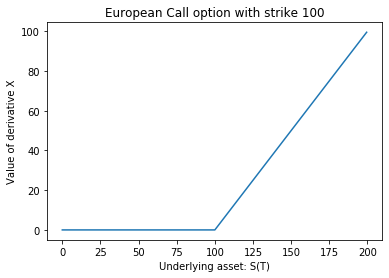
\includegraphics{Figures/euroCall.png}
\decoRule
\caption[]{European call with K=100}
\label{fig:EuroCall}
\end{figure}

The European put is very similar to the call, except now we earn, when the stock is below the strike price K.\\
$\Phi(S(T))=max(K-S,0)$.
\begin{figure}[h]
\centering
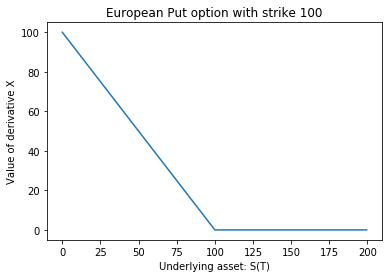
\includegraphics{Figures/euroPut.png}
\decoRule
\caption[]{European put with K=100}
\label{fig:EuroPut}
\end{figure}
\chapter{Code Implementation} % Main appendix title

\label{AppendixB} % Change X to a consecutive letter; for referencing this appendix elsewhere, use \ref{AppendixX}

The code is available at my GitHub repository \href{https://github.com/MrPPL/DeepPricing}{https://github.com/MrPPL/DeepPricing}. The code is written in the python directory and the following files are used:
\begin{enumerate}
\item[•] European call and put option:\\
ClosedForm directory and the file closedEuro.py
\item[•] Exotic European options:\\
ClosedForm directory and the file rainbow2Dim.py
\item[•] CRR:\\
Directory BinomialModel and file BinoHull.py
\item[•] BEG:\\
Directory BinomialModel and file BEGTwoDim.py
\item[•] LSM:\\
Directory DeepStopping and file AmericanPut.py\footnote{Note that the LSM is implemented by using luphord GitHub repository \href{https://github.com/luphord/longstaff_schwartz}{https\:\/\/github.com/luphord/longstaff\_schwartz}}
\item[•] MLPs I:\\
Directory DeepStopping and file AmericanPut.py \footnote{Note that the MLPs is my own build upon the LSM method}
\item[•] MLPs II:\\
Directory DeepLearning/hirsa19/evaluation and file MLPsIIPricing.py
\end{enumerate}
% Appendix Template

\chapter{Additional Material for CRR, LSM, and MLP I} % Main appendix title

\label{AppendixC} % Change X to a consecutive letter; for referencing this appendix elsewhere, use \ref{AppendixX}

\section{Moment Matching CRR}\label{CRRMM}
In the CRR the stock multiplication factor for up and down movement is chosen to match the two first moments of the lognormal distribution. By matching the first moments the underlying discrete binomial stochastic process for the stock converge toward the continuous time lognormal distribution for sufficient large equidistant time-steps N. Hence, the CRR model will coincide with the Black-Scholes model.\\

The SDE for the Black Scholes under the equivalent martingale measure Q:
$$dS(t)=rS(t)dt + \sigma S(t) dW(t)$$
Using Itô's lemma:
\begin{equation}\label{lnGBM}
d\ln(S(t)))=(r-\frac{1}{2}))dt + \sigma dW_t
\end{equation}
The solution of equation \ref{lnGBM} is then:
$$S(t)=S(0)\exp\bigg((r-\dfrac{1}{2}\sigma)t+ \sigma W(t) \bigg)$$
Note that $W(t)\sim \mathcal{N}(0,t)$ implies:
$$\ln(\dfrac{S(t)}{S(0)}) \sim \mathcal{N}((r-\dfrac{1}{2}\sigma^2)t, \sigma^2 t)$$
The two first moments for the lognormal distribution are then:
\begin{equation}\label{lnMoments}
\begin{split}
E[\dfrac{S(t)}{S(0)}]=\exp(rt)\\
E[(\dfrac{S(t)}{S(0)})^2]=\exp(t\cdot (2r + \sigma^2))
\end{split}
\end{equation}
The above derivation can be used for any time interval.\\

The binomial lattice model has two discrete outcomes from each state and the moments are:
\begin{equation}\label{binMoments}
\begin{split}
E[\dfrac{S(t_{n+1})}{S(t_{n})}]=u \cdot Q(\dfrac{S(t_{n+1})}{S(t_{n})} = u) + d \cdot Q(\dfrac{S(t_{n+1})}{S(t_{n})} = d) = u \cdot q + d \cdot (1-q)\\
E[(\dfrac{S(t_{n+1})}{S(t_{n})})^2]=u^2 \cdot q + d^2 \cdot (1-q)
\end{split}
\end{equation}
We match the moments (equations \eqref{lnMoments} and \eqref{binMoments}) and get two equations with two unknowns, where the time-step is chosen to be $\Delta t$
\begin{align*}
\exp(r \Delta t)=u \cdot q + d \cdot (1-q) \quad (i)\\
\exp(\Delta t \cdot (2r + \sigma^2))=u^2 \cdot q + d^2 \cdot (1-q) \quad (ii)
\end{align*}
Multipling $(i)$ with u+d and recognizing $(ii)$:
\begin{align*}
(u+d)\exp(r \Delta t)&=u^2 \cdot q + d^2 \cdot (1-q) + ud\\
\Rightarrow (u+d)\exp(r \Delta t)&\overset{(ii)}{=}\exp(\Delta t \cdot (2r + \sigma^2)) + u d
\end{align*}
Remember, we choose $u= \frac{1}{d}$ and arrive at a quadratic equation through algebra.
\begin{align*}
u^2 - u\bigg(\exp(-r \Delta t) + \exp(\Delta t(r+\sigma^2))\bigg)+1=0
\end{align*}
We are interested in that the binomial model converge toward the Black-Scholes model. Therefore, we are looking at small time increment $\Delta t$. This justify the Taylor approximation of the exponential function around zero.
\begin{align*}
\exp(r \Delta t + \sigma^2 \Delta t) \approx 1 + (r+\sigma^2)\Delta t + O(t^2)
\end{align*}
By Taylor approximation we arrive at a simpler quadratic equation:
\begin{equation*}
u^2-u(2+\sigma^2 \Delta t) + 1 = 0
\end{equation*}
Solving the quadratic equation above gives:
\begin{align*}
u&=1+\dfrac{1}{2} \sigma^2 \Delta t \pm  \dfrac{\sqrt{(2+\sigma^2 \Delta t)^2 - 4}}{2}\\
&=1+\dfrac{1}{2} \sigma^2 \Delta t \pm  \dfrac{\sqrt{(4+\sigma^4 \Delta t^2 + 4 \sigma^2 \Delta t - 4}}{2}\\
&=1+\dfrac{1}{2} \sigma^2 \Delta t \pm \frac{1}{2} \sigma \sqrt{\Delta t} \sqrt{\sigma^2 \Delta t + 4}\\
&\approx 1+\dfrac{1}{2} \sigma^2 \Delta t \pm \sigma \sqrt{\Delta t}\\
&\approx \exp(\pm \sigma \sqrt{\Delta t})
\end{align*}
Both approximations exploit that the time-step is small.
\section{Convergence for LSM and MLP I}\label{Convergence}
\subsection{LSM}
In the rigorous approach in \parencite{analysisLSM} they show convergence results for the optimal value process or the Snell envelope $U$. We will present that $U(0)^{m,K}$ converges almost surely to $U(0)^{m}$ for K goes to infinity, i.e. the approximate value process by simulation and regression on a finite set of functions converge to the approximated value process with truncated orthogonal basis by letting the sample size go to infinity. Furthermore, it can be shown that $U(0)^{m}$ converges to $U(0)$ for m goes to infinity. The second result is that the regressed value function converges to the expected continuation value by letting the number of basis functions go to infinity. The latter result is shown using the expected continuation values.
\begin{theorem}\label{LSMConvergence1}
Assume the sequence $(e_{j}(S(t_n)))_{j\geq 1}$ is total in $L^2(\sigma(S(t_n)))$ for $n=1,\ldots,N-1$. Then for $n=0,\ldots,N$ we have
$$\lim_{m\to +\infty} E^Q[G(S(\tau_{t_n}^{[m]})) |\mathcal{F}_{t_n}]=E^Q[G(S(\tau_{t_n})) |\mathcal{F}_{t_n}]$$
in $L^2$
\begin{proof}
The proof is given by induction, where the orthogonal basis is total in $L^2$ is important because $||P^m_{t_n}(E^Q[G(S(\tau_{t_{n+1}}))|\mathcal{F}_{t_n}])- E^Q[G(S(\tau_{t_{n+1}}))|\mathcal{F}_{t_n}]||_2 \to 0 \quad for \ m \to \infty$.
(more details on p. 6-7 \parencite{analysisLSM})
\end{proof}
\end{theorem}

The former result is also shown in \parencite{analysisLSM}.
\begin{theorem}\label{LSMConvergence2}
Assume the sequence $(e_{j}(S(t_n)))_{j\geq 1}$ is total in $L^2(\sigma(S(t_n)))$ for $n=1,\ldots,N-1$ and if $\sum_{j=1}^{m} \lambda_j e_{j}(S(t_n))=0 \ a.s.$ then $\lambda_j=0$ for $n=1,\ldots,N-1$, $m\geq 1$ and $j=1,\ldots,m$. Furthermore assume that $Q(\alpha_{t_n} \cdot e(S(t_n))=G(S(t_n)))=0$.\\
Then $U^{m,K}(0)$ converges almost surely to $U^{m}(0)$ as K goes to infinity.\\
The proof is out of scope for this thesis, see the article \parencite{analysisLSM} for a proof in details. 
\end{theorem}

The two convergence results show the convergence for the LSM algorithm, hence, the LSM will approximate the optimal value process well for sufficiently large sample sets and enough basis functions.

\subsection{MLP I}
The MLP regression method enjoys the same convergence results presented for the LSM algorithm, i.e.
\begin{theorem}\label{NNConvergence1}
Assume that 
$$E[\max_{0\leq t_n \leq T} |G(S(t_n))|^2]< \infty$$. 
Then $\lim_{p \to \infty} E^Q[G(S(\tau^{p}_{t_n}))| \mathcal{F}_{t_n}]= E[G(\tau_{t_n})|\mathcal{F}_{t_n}]$ in $L^2(\Omega)$ for all $n \in \{1,2,\ldots, N\}$\\
Proof p. 7-8 \parencite{Lelong19}
\end{theorem}
The above theorem states convergence of the neural network approximation, i.e. $U^{p}(0) \to U(0)$ which is similar to the convergence result for LSM. 
\begin{theorem}{\textbf{Strong law of large numbers: }}\label{NNConvergence2}
Assume
\begin{enumerate}
\item[A1:] For every $p\in \mathbb{N}$, $p>1$, there exist $q \geq 1$ and $\kappa_p>0$ such that
$$\forall s \in \mathbb{R}^{R}, \forall \theta \in \Theta_p, \quad |\Psi_p(s,\theta)| \leq \kappa_p (1+|s|^q) $$
Moreover $\forall n \in \{1,2,\ldots, N-1\}$, a.s. the random functions $\theta \in \Theta_p \mapsto \Psi_p(S(t_n), \theta)$ are continuous. Note $\Theta_p$ is a compact set, hence, the continuity is uniform.
\item[A2:] For $q$ defined in A1, $E^Q[|S(t_n)|^{2q}]<\infty \quad \forall n \in \mathbb{N} \cup 0$
\item[A3:] $\forall p \in \mathbb{N}$, $p>1$ and $\forall n \in \{1,2,\ldots, N-1\}$, 
$$P(S(t_n)=\Psi_{p}(S(t_n);\theta_{t_n}^{p})=0$$
\item[A4:] $\forall p \in \mathbb{N}$, $p>1$ and $\forall n \in \{1,2,\ldots, N-1\}$, if $\theta^{1}$ and $\theta^{2}$ solves 
\begin{align*}
\argmin_{\theta \in \Theta_p} E^Q[|\Psi_p(S(t_n); \theta)- S(\tau_{t_{n+1}}^{p})|^2]
\end{align*}
then $\Psi_p(s,\theta^{1})=\Psi_p(s,\theta^{2})$ for almost all x.
\end{enumerate}
If A1-A4 hold, then for $\zeta\in \{1,2\}$ and every $n\in \{1,2,\ldots,N\}$
\begin{equation}
\lim_{K\to \infty} \dfrac{1}{K} \sum_{k=1}^{K} \bigg(G(S(\hat{\tau}_{t_n}^{k,p,K}))\bigg)^{\zeta} = E[\bigg(G(S(\tau_{t_n}^{p}))\bigg)^{\zeta}] \quad a.s.
\end{equation}
Proof p. 13-14 \parencite{Lelong19}
\end{theorem}
The last result is the strong law of large numbers for the value function, i.e. $U^{p,K}(0) \to U^{p}(0) \ a.s. \quad for \ K \to \infty$

\section{LSM Lower Bound}\label{LSMLowerBound}
The LSM approach gives a lower bound for the true price of the option given optimal stopping choice:
\theoremstyle{proposition}
\begin{proposition}{\textbf{Lower Bound To True Value: }}\label{Lower-Bound-LSM}
For any finite choice of M, K, and vector $\theta\in \mathbb{R}^{M \times (K-1)}$ representing the coefficients for the M basis functions at each of the K-1 early exercise dates, let $LSM(\omega;M,K)$ denote the discounted cash flow resulting from the following the LSM rule of exercising when the immediate exercise value is positive and greater than or equal to $\hat{F}_{M}(\omega_{l};t_{k})$ as defined by $\theta$. Then the following inequality almost surely holds,
$$V(X)\geq \lim_{N\to \infty} \dfrac{1}{N}\sum_{i=1}^{N} LSM(\omega_i;M,K)$$
\null \hfill (p. 124 \parencite{LSM})
\end{proposition}
% Appendix D

\chapter{Additional Tables and Figures} % Main appendix title

\label{AppendixD} % For referencing this appendix elsewhere, use \ref{AppendixA}

\section{Tables}

\begin{table}[H]
\caption{Polynomial Regression for European Call}{Polynomial regression result for the European call option}
\label{tab:fullEuroCall}
\centering
\begin{tabular}{llllllll}
\toprule
\textbf{Data set} &  \textbf{Measure} & \textbf{1. degree} & \textbf{2. degree} & \textbf{3. degree} & {4. degree} & \textbf{5. degree} & {6. degree}\\
\midrule
In-Sample     &	MSE  & 0.000636 & 0.000069 & 0.000013 & 0.000004 & 0.000002 & 0.000001 \\
		      & RMSE & 0.025212 & 0.008316 & 0.003624 & 0.002052 & 0.001414 & 0.000958 \\
		      & MAE  & 0.018326 & 0.006141 & 0.002561 & 0.001280 & 0.000867 & 0.000591 \\
		      & $R^2$& 0.936628 & 0.993105 & 0.998691 & 0.999580 & 0.999801 & 0.999909 \\
Long Maturity & MSE  & 0.002662 & 0.001196 & 0.001654 & 0.003956 & 0.012255 & 0.043361 \\
		      & RMSE & 0.051593 & 0.034577 & 0.040666 & 0.062894 & 0.110702 & 0.208233 \\
		      & MAE  & 0.041232 & 0.026287 & 0.028371 & 0.039932 & 0.064402 & 0.111190 \\
		      & $R^2$& 0.818143 & 0.918316 & 0.887014 & 0.729744 & 0.162742 & -1.962442 \\
Out-of-Money  & MSE  & 0.005772 & 0.000767 & 0.000839 & 0.000944 & 0.001812 & 0.004423 \\
		      & RMSE & 0.075973 & 0.027694 & 0.028960 & 0.030724 & 0.042568 & 0.066506 \\
		      & MAE  & 0.060936 & 0.022203 & 0.020288 & 0.020542 & 0.027125 & 0.041315\\
		      & $R^2$& -2.377251 & 0.551246 & 0.509280 & 0.447668 & -0.060261 & -1.588030\\
\bottomrule\\
\end{tabular}
\end{table}

\begin{table}[H]
\caption{Grid Search for American Bivariate Contingent Claim}{Hyperparameter tuning of dataset size and batch size for American put minimum two assets, for the interested reader see the tensorboard}
\label{tab:fullhyperAmerMin4}
\centering
\begin{tabular}{llll}
\toprule
\textbf{Data set Size} & \textbf{$\eta$} & \textbf{Batch Size} & \textbf{Loss} \\
\midrule
300K    & 0.0001 & 8     & 0.015130897983909 \\ 
300K    & 0.001  & 64    & 0.035523075610399 \\ 
100K    & 0.0001 & 8     & 0.064886227250099 \\ 
100K    & 0.001  & 8     & 0.072143875062466 \\ 
300K    & 0.0001 & 64    & 0.075988814234734 \\ 
300K    & 0.001  & 8     & 0.104622706770897 \\ 
300K    & 0.01   & 256   & 0.480043411254883 \\ 
300K    & 0.0001 & 256   & 1.04093873500824  \\ 
300K    & 0.001  & 256   & 1.06809389591217  \\ 
300K    & 0.001  & 512   & 1.08942472934723  \\ 
100K    & 0.001  & 64    & 1.18230485916138  \\ 
300K    & 0.001  & 1024  & 1.30065310001373  \\ 
300K    & 0.01   & 512   & 1.45135951042175  \\ 
100K    & 0.01   & 256   & 1.52623510360718  \\ 
300K    & 0.01   & 64    & 1.75954759120941  \\ 
300K    & 0.01   & 1024  & 1.92213356494904  \\ 
100K    & 0.01   & 512   & 2.01193928718567  \\ 
100K    & 0.01   & 64    & 2.02969717979431  \\ 
300K    & 0.0001 & 1024  & 5.72439670562744  \\ 
300K    & 0.0001 & 512   & 5.72847843170166  \\ 
100K    & 0.0001 & 256   & 5.76278400421143  \\ 
100K    & 0.0001 & 512   & 5.77397203445435  \\ 
100K    & 0.0001 & 64    & 5.80239868164063  \\ 
100K    & 0.0001 & 1024  & 5.90070772171021  \\ 
100K    & 0.001  & 256   & 6.29003953933716  \\ 
100K    & 0.001  & 512   & 6.52896738052368  \\ 
100K    & 0.001  & 1024  & 6.56187915802002  \\ 
1K      & 0.001  & 8     & 7.5845251083374   \\ 
100K    & 0.01   & 8     & 8.07239627838135  \\ 
1K      & 0.01   & 8     & 11.7414264678955  \\ 
100K    & 0.01   & 1024  & 13.4287099838257  \\ 
1K      & 0.01   & 64    & 14.1254253387451  \\ 
1K      & 0.0001 & 8     & 24.0087566375732  \\ 
1K      & 0.001  & 64    & 27.0112972259521  \\ 
1K      & 0.01   & 512   & 40.0226554870605  \\ 
1K      & 0.001  & 512   & 44.841724395752   \\ 
1K      & 0.01   & 256   & 45.8363571166992  \\ 
1K      & 0.01   & 1024  & 49.3933792114258  \\ 
1K      & 0.0001 & 64    & 51.3070755004883  \\ 
1K      & 0.001  & 256   & 52.8623466491699  \\ 
1K      & 0.0001 & 512   & 87.4313125610352  \\ 
1K      & 0.0001 & 256   & 89.8093795776367  \\ 
1K      & 0.0001 & 1024  & 90.8342361450195  \\ 
\bottomrule\\
\end{tabular}
\end{table}




\section{Figures}

\begin{figure}[H]
\centering
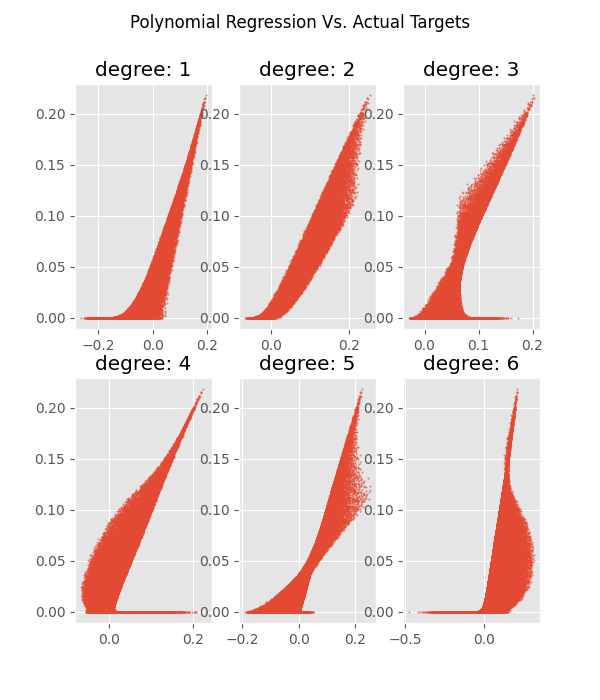
\includegraphics{Figures/polynomialOutMoneyEuroC.png}
\decoRule
\caption[Polynomial Regression Performance for Out-of-money Data Set European Call]{Polynomial regression performance for out of money data set on the European call}
\label{fig:MLPsEuroCOutOfMoney}
\end{figure}

\begin{figure}[th]
\centering
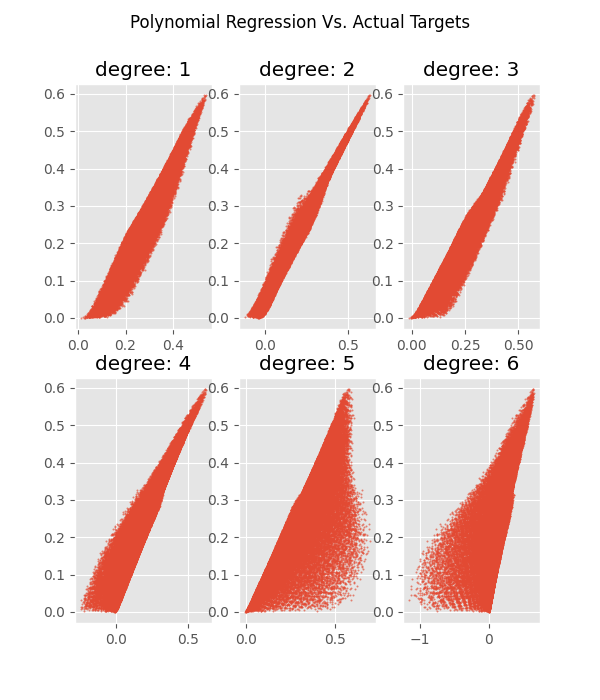
\includegraphics{Figures/polynomialLongTEuroC.png}
\decoRule
\caption[Polynomial Regression Performance for Long Maturity Data Set European Call]{Polynomial regression performance for long maturity data set on European call}
\label{fig:MLPsEuroCLongMaturity}
\end{figure}


\begin{figure}[th]
\centering
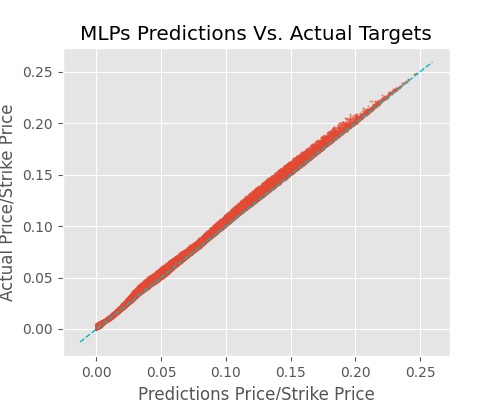
\includegraphics{Figures/outMoneyAmerP.png}
\decoRule
\caption[MLPs Performance for In-the-Money Data Set American Put]{MLPs performance for in-the-money data set on American put}
\label{fig:MLPsAmerPOutMoney}
\end{figure}

\begin{figure}[th]
\centering
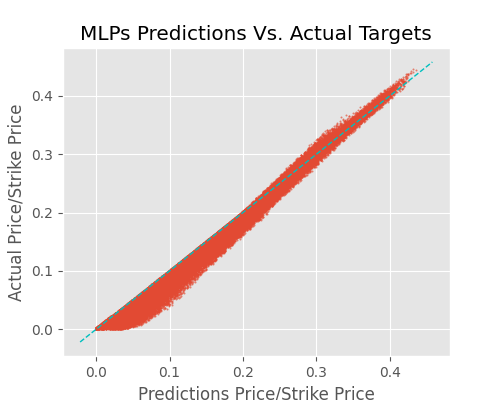
\includegraphics{Figures/longTAmerP.png}
\decoRule
\caption[MLPs Performance for Long Maturity Data Set American Put]{MLPs performance for long maturity data set on American put}
\label{fig:MLPsAmerPLongT}
\end{figure}

\begin{figure}[th]
\centering
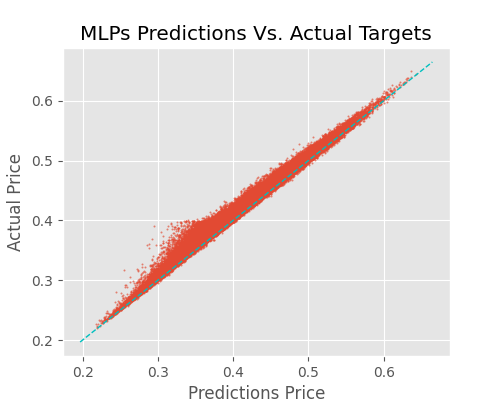
\includegraphics{Figures/inMoneyAmerMinP.png}
\decoRule
\caption[MLPs Performance for In-the-Money Data Set Bivariate American Contingent Claim]{MLPs performance on in-the-money data set on American put on minimum of two stocks}
\label{fig:MLPsAmerMin2}
\end{figure}

\begin{figure}[th]
\centering
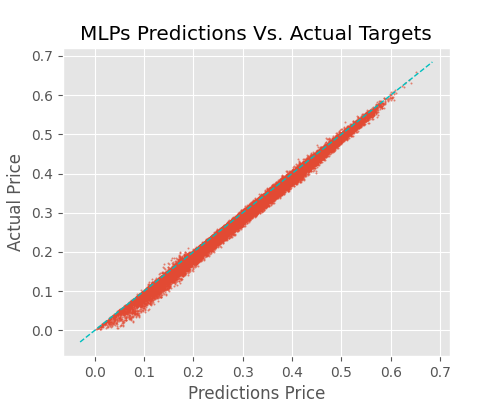
\includegraphics{Figures/longTAmerMinP.png}
\decoRule
\caption[MLPs Performance for Long Maturity Data Set Bivariate American Contingent Claim]{MLPs performance for long maturity data set on American put on minimum of two stocks}
\label{fig:MLPsAmerMin1}
\end{figure}








%----------------------------------------------------------------------------------------
%	BIBLIOGRAPHY
%----------------------------------------------------------------------------------------




\printbibliography[heading=bibintoc]

%----------------------------------------------------------------------------------------

\end{document}  








Batch normalization\\
Important to standardize the covariates. And highly correlated covariates should be trimmed down.
It is also a good idea to standardize the hidden covariates as well. This is called batch normalization and can accelarate the training of a network considerably.\\

It is recommended to use batch normalization  in combination with dropout. \\


By using a dynamic programming argument with three strategies:
\begin{enumerate}
\item[•] Use optimal stopping strategy $\hat{\tau}_t$
\item[•] Stop immediately
\item[•] Wait one time-step h and then use optimal stopping strategy $\hat{\tau}_{t+h}$
\end{enumerate}

We will see in the American put section why these two propositions are useful. 

By following the arguments in section 25 in \parencite{Shiryaev06}, we arrive at two important propositions for numerically evaluating American options.

\begin{proposition}{\textbf{variational inequalities}}\label{varInEq}
Given enough regularity, the optimal value function is characterized by the following relations:
\begin{equation}
\begin{split}
V(T,x)=\Phi(T,x)\\
V(t,x)\geq \Phi(t,x) \quad \forall (t,x)\\
\bigg(\frac{\partial}{\partial t} + \mathbb{A}\bigg)V(t,x) \leq 0 \quad \forall (t,x)\\
\max\bigg\{V(t,x) - \Phi(t,x), \bigg(\frac{\partial}{\partial t} + \mathbb{A}\bigg)V(t,x) \bigg\} = 0 \quad \forall (t,x)\\
\textsl{Where $\mathbb{A}$ is the Itô operator:}\\
\mathbb{A}f(t,x) =  \mu(t,x) \frac{\partial f(t,x)}{\partial x} + \frac{1}{2} \sigma^2(t,x) \frac{\partial^2 f(t,x)}{\partial x^2}
\end{split}
\end{equation}
(see p. 344 \parencite{finKont})
\end{proposition}

\begin{proposition}{\textbf{Free boundary value problem}}\label{freeBoundary}
Assuming enough regularity, the optimal value function satisfies the following parabolic equation
\[ \begin{cases} 
      \frac{\partial V(t,x)}{\partial t}(t,x) + \mu(t,x) \frac{\partial V(t,x)}{\partial x}(t,x) + \frac{1}{2}\sigma^2(t,x)\frac{\partial^2 V(t,x)}{\partial x^2}=0 & (t,x)\in C \\
     V(t,x)=\Phi(t,x)  & (t,x)\in \partial C \\
   \end{cases}
\]
Where C is the continuation region defined by:
$$C=\{(t,x): V(t,x)>\Phi(t,x) \}$$
(see p. 343-344 \parencite{finKont})
\end{proposition}

The two propositions can be used to value american put options numerically, but we will take an different approach in this thesis.
So for practical use there are three strategies to find the fair price for the option:
\begin{enumerate}
\item[•] Solve the free boundary free problem numerically (see \ref{freeBoundary})
\item[•] Solve the variational inequalities numerically (see \ref{varInEq})
\item[•] Approximate the Black-Scholes model by a binomial model and compute the exact binomial American put price.\\
(p. 347 \parencite{finKont})
\end{enumerate}

At maturity the cash flow from the option is the same as for an European put option, hence the cash flow from each path is $G(S(T))=max(K-S_T,0)$. We use the notation $G(S(\tau_{t+1}))$ denote the path of cash flows generated by the option condition on the option not being exercised before t and the option holder follow the optimal stopping strategy for all s, $t<s\leq T$.
(inspired by \parencite{lsm} p. 121). The continuation value is given by:
\begin{equation}\label{continuation-value}
\begin{split}
F(\omega; t_n)=E^Q[\sum_{j=n+1}^N \exp(-\int_{t_n}^{t_j} r(\omega,s) ds) G(S(\tau_{t+1})) |\mathcal{F}_{t_k}]
\end{split}
\end{equation}
where $r(\omega,t)$ is risk free interest rate, and the $\mathcal{F}_{t_k}$ is the filtration at time $t_k$.\\

We get the optimal stopping strategy by comparing thr continuation value with the intrinsic value at each time step. By working backward in time until the initialization of the option, we have approximated the the optimal stopping times and the cash flows associated with exercising at the optimal stopping times

To estimate the condition expectation in equation \ref{continuation-value}, we regres with the basis functions taking on the underlying asset for the option being the independent variable:
 \parencite{lsm}.
 
 \begin{equation*}
\begin{split}
S_i(t)=S_i(0) \cdot \exp \bigg( \sum_{j=1}^{d}(\sigma_{i,j} W_j(t) -\frac{1}{2} \sigma_{i,j}^2 t) + rt \bigg) \quad  for \ i=1,\ldots,d
\end{split}
\end{equation*}
Where the Wiener processes are independent and its domain in $\mathbb{R}^+$.
